%Einbinden der Dokumentenklasse und der Pakete
\documentclass[paper=a4, fontsize=12pt]{scrreprt}


% ========== Pakete einbinden ==========
\usepackage[english]{babel}
\usepackage[utf8]{inputenc}        
\usepackage[T1]{fontenc}             % f�r "modernere" Schriftkodierung
\usepackage{csquotes} 
\usepackage[intlimits]{amsmath}      % f�r erweiterte mathematische Konstrukte
\usepackage{amsfonts}                % f�r erweiterte mathematische Schriften
\usepackage{amssymb}                 % f�r erweiterten Symbolvorrat
\usepackage{amsthm}
\usepackage{typearea}                % f�r die Berechnung der Seitenr�nder
\usepackage{array}                   % f�r erweiterte Tabellensatzm�glichkeiten
\usepackage{enumerate}               % f�r komfortablere Aufz�hlungen
\usepackage[shortlabels]{enumitem}	 %anständige enumerate Umgebung
\usepackage{fancyhdr}
\usepackage{latexsym}
\usepackage{graphicx}
\usepackage{mathtools}
\usepackage[plainpages=false,pdfpagelabels]{hyperref}
\usepackage[left=2.5cm,right=2.5cm,top=1.5cm,bottom=2.5cm,includeheadfoot]{geometry}
\usepackage{cleveref}
\usepackage{tikz}
\usetikzlibrary{cd, matrix,arrows,decorations.pathmorphing, babel}
\usepackage[disable]{todonotes}
\usepackage{marvosym} %Lightning
%\usepackage{MnSymbol} %enthält \leftmapsto
\usepackage{stmaryrd} %enthält \leftmapsfrom
\usepackage{lastpage}
\usepackage{tikz-cd}
\usepackage{pdfpages}

\hypersetup{pdftitle=, 
            pdfauthor={Sascha Blug, Ricardo Schnur, Christian Steinhart},
    colorlinks,
    linkcolor=black,
    citecolor=black,
    urlcolor=blue
}

\allowdisplaybreaks[3]				% Zeilenumbruch in align etc [x], x=1,...,4

\parindent 0pt

%Einbinden eigener Befehle
% ---------- Definitionen, Sätze, ... ----------

\theoremstyle{definition}
\newtheorem{defi}{Definition}
\newtheorem{Not}[defi]{Notation}

\theoremstyle{plain}
\newtheorem{Satz}[defi]{Theorem}
\newtheorem{Lem}[defi]{Lemma}
\newtheorem{Kor}[defi]{Corollary}
\newtheorem{Prop}[defi]{Proposition}
\newtheorem*{conjecture*}{Conjecture}
\newtheorem{Lemdef}[defi]{Lemma and Definition}

\theoremstyle{remark}
\newtheorem{Bem}[defi]{Remark}
\newtheorem*{Bem*}{Remark}
\newtheorem{Bemdef}[defi]{Remark and Definition}
\newtheorem{Bsp}[defi]{Example}
\newtheorem*{Bsp*}{Example}
\newtheorem{idea}[defi]{Idea}
\newtheorem{prob}[defi]{Problem}
\newtheorem{remin}[defi]{Reminder}

     
\numberwithin{defi}{section}
            
    
% ---------- Mengen, Buchstaben, ... ----------

\newcommand{\N}{\mathbb{N}}
\newcommand{\Z}{\mathbb{Z}}
\newcommand{\Q}{\mathbb{Q}}
\newcommand{\R}{\mathbb{R}}
\newcommand{\C}{\mathbb{C}}
\let\k\relax
\newcommand{\k}{\mathbb{K}}
\newcommand{\Aff}{\mathbb{A}}

\newcommand{\Pot}{\mathcal{P}}

\let\P\relax
\newcommand{\P}{\mathbb{P}}

\newcommand{\E}{\mathcal{E}}
\newcommand{\F}{\mathcal{F}}
\newcommand{\G}{\mathcal{G}}

\newcommand{\A}{\mathcal{A}}
\newcommand{\B}{\mathcal{B}}

\let\O\relax
\newcommand{\O}{\mathcal{O}}


\newcommand{\X}{\mathscr{X}}
\newcommand{\U}{\mathcal{U}}
\newcommand{\LC}{\mathcal{L}}

\newcommand{\K}{\mathcal{K}}
\newcommand{\D}{\mathbb{D}}

\newcommand{\J}{\mathcal{J}}
\newcommand{\PP}{\mathcal{P}}


% ---------- Funktionen ----------

\newcommand{\abs}[1]{\left|{#1}\right|}
\newcommand{\norm}[1]{\left\|{#1}\right\|}
\newcommand{\ceil}[1]{\left\lceil {#1} \right\rceil}
\newcommand{\floor}[1]{\left\lfloor {#1} \right\rfloor}
\newcommand{\set}[2]{\left\{ {#1} \bigm| {#2} \right\}}


% ---------- MathOperators ----------

\let\Re\relax
\let\Im\relax
\DeclareMathOperator{\Re}{Re}
\DeclareMathOperator{\Im}{Im}
\DeclareMathOperator{\Int}{Int}
\DeclareMathOperator{\Gl}{Gl}
\DeclareMathOperator{\Var}{Var}
\DeclareMathOperator{\Cov}{Cov}
\DeclareMathOperator{\Corr}{Corr}
\DeclareMathOperator{\Mat}{Mat}
\DeclareMathOperator{\GL}{GL}
\DeclareMathOperator{\SL}{SL}
\DeclareMathOperator{\Sp}{Sp}
\DeclareMathOperator{\ind}{ind}
\DeclareMathOperator{\res}{res}
\DeclareMathOperator{\supp}{supp}
\DeclareMathOperator{\Syz}{Syz}
\DeclareMathOperator{\sgn}{sgn}
\DeclareMathOperator{\diam}{diam}
\DeclareMathOperator{\ord}{ord}
\DeclareMathOperator{\spec}{spec}
\DeclareMathOperator{\Bild}{Bild}
\DeclareMathOperator{\dist}{dist}
\DeclareMathOperator{\rg}{rg}
\DeclareMathOperator{\tr}{tr}
\DeclareMathOperator{\diag}{diag}
\DeclareMathOperator{\id}{id}
\DeclareMathOperator{\spanset}{span}
\DeclareMathOperator{\LH}{LH}
\DeclareMathOperator{\proj}{proj}
\DeclareMathOperator{\Log}{Log}
\DeclareMathOperator{\ggT}{ggT}
\DeclareMathOperator{\Quot}{Quot}
\DeclareMathOperator{\Hom}{Hom}
\DeclareMathOperator{\Gal}{Gal}
\DeclareMathOperator{\Norm}{\mathcal{N}}
\DeclareMathOperator{\Tr}{Tr}
\DeclareMathOperator{\TrL}{\Tr_{L/K}}
\DeclareMathOperator{\NormL}{\mathcal{N}_{L/K}}
\DeclareMathOperator{\rank}{rank}
\DeclareMathOperator{\Cl}{Cl}
\DeclareMathOperator{\vol}{vol}
\DeclareMathOperator{\can}{can}
\DeclareMathOperator{\Leb}{Leb}
\DeclareMathOperator{\volcan}{\vol_{can}}
\DeclareMathOperator{\volLeb}{\vol_{\Leb}}


% ---------- Sonstiges ----------

\newcommand{\td}{\,\mathrm{d}}
\newcommand{\bs}{\backslash}



\begin{document}

\pagestyle{fancy}
\cfoot{\thepage \ / \pageref{LastPage}}
\lhead{WS 17/18}
\chead{Algebraic Number Theory}


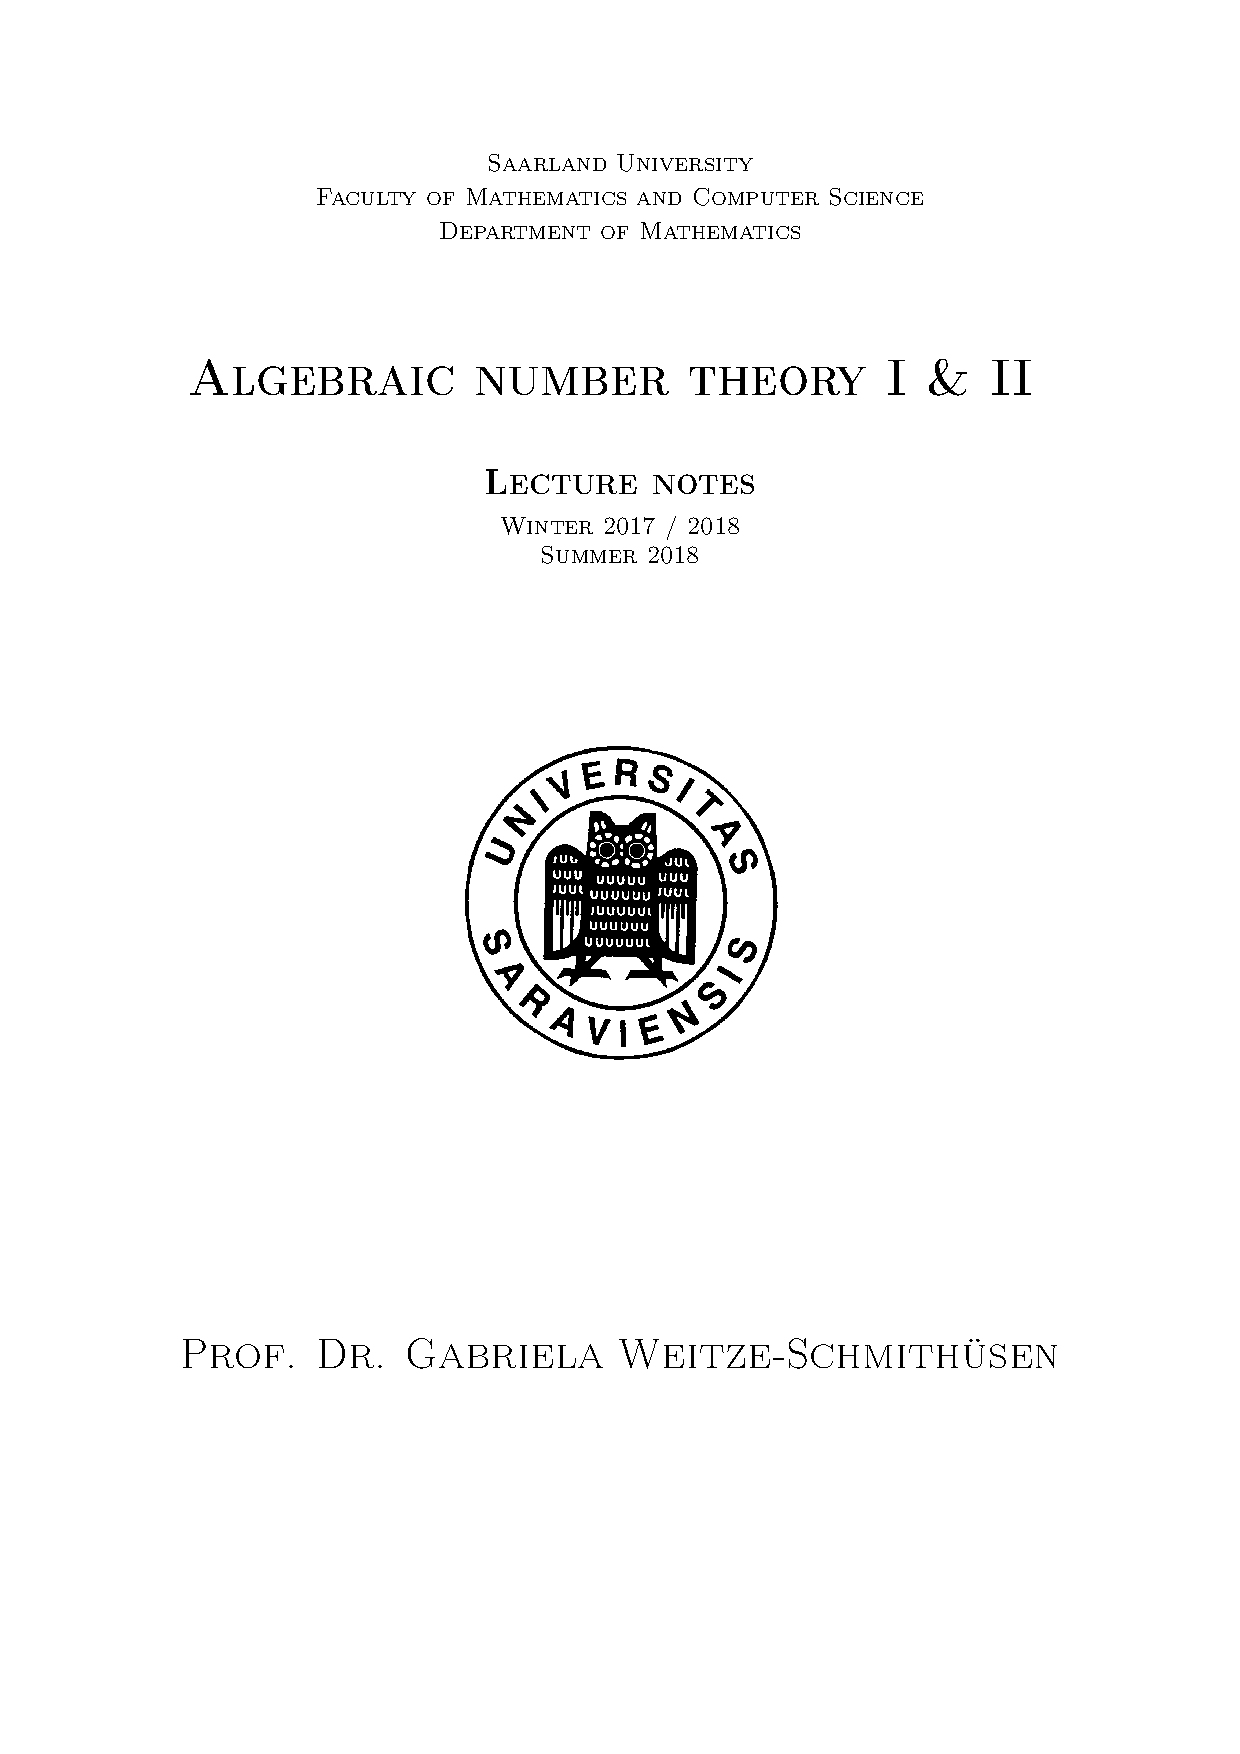
\includepdf{cover/cover.pdf}
\renewcommand{\contentsname}{Table of contents}
\tableofcontents


\rhead{23 October 2017}

\chapter{Small prefix}

\underline{Recall:}
\begin{itemize}
\item $L$ numberfield $:\iff$ $L$ is a finite extension of $\Q$\\
In particular: $L / \Q$ is separable $\Rightarrow L/\Q$ is primitive, i.e. $L=\Q(\alpha), \Q[X] \ni f_\alpha=$ minimal polynomial of $\alpha$ over $\Q$ and $[L:\Q]=\deg(f_\alpha)$.
\item $\O:=\{\alpha \in L \ | \ f_\alpha \in \Z[X]\}$ is called \emph{ring of integers} (generalization of $\Z \subseteq \Q$).\\
$\O$ is an integral domain.
\item \underline{Goal:} study the ring $\O$
\item \underline{Questions:} \begin{enumerate}
\item What is $\O^\times$? What is its structure?
\item What are the prime ideals of $\O$?
\item Do we have a unique prime factorization, i.e. is $\O$ a UFD?
\end{enumerate}
\end{itemize}

\section{Motivation}
\begin{prob}[Fermat's conjecture, $\sim$ 1640]
Show that the equation $x^n+y^n=z^n$ has no nontrivial integer solutions, i.e. solutions $(x,y,z)$ with $x,y,z \in \Z\setminus \{0\}$ for $n \geq 3$.
\end{prob}
\underline{History:} \begin{itemize}
\item 1770: Euler found solution for $n=3$
\item 1825: Dirichlet and Legendre using Germain \todo{??}
\item Kummer showed it for many primes, he showed as well that his idea doesn't work for all $n \in \N_{>2}$
\item Conjecture was proved by Wiles in 1997
\end{itemize}

\begin{Bem}
\begin{enumerate}[i)]
\item If Fermat's is true for $n$, then also for $nk$ for all $k \in \N$.
\item It is sufficient to prove Fermat's conjecture for $n=4$ and all odd primes.
\end{enumerate}
\end{Bem}
\begin{proof}
\begin{enumerate}[i)]
\item Suppose $(x,y,z)$ is a nontrivial solution of $x^{nk}+y^{nk}=z^{nk} \Rightarrow (x^k,y^k,z^k)$ is a nontrivial solution to $x^n+y^n=z^n$.
\item Follows from i).
\end{enumerate}
\end{proof}

\begin{Prop}[$n=2$]
Suppose $x,y,z \in \Z, \gcd(x,y,z)=1$
\begin{enumerate}[i)]
\item $x,y,z$ are pairwise coprime if $x^2+y^2=z^2$
\item $x^2+y^2=z^2 \Rightarrow$ either $x$ or $y$ is even
\item $x^2+y^2=z^2 \iff \exists \ r,s \in \N_0, \gcd(r,s)=1$ s.t. $x=\pm 2rs, y= \pm (r^2-s^2), \linebreak
z = \pm(r^2+s^2)$.
\end{enumerate}
\end{Prop}
\begin{proof}
\begin{enumerate}[i)]
\item clear \checkmark
\item One of $x,y,z$ has to be even, since $odd+odd \neq odd$. Suppose $z$ is even. Then look at equation $\mod 4$, this gives a contradiction. By i) only one of $x$ and $y$ is even.
\item \glqq $\Leftarrow$\grqq: calculation\\
\glqq $\Rightarrow$\grqq: Wlog. assume $x,y,z \in \N_0,\ x$ even, $y,z$ odd:
\begin{align*}
\ \ &\Rightarrow x=2u, z+y=2v, z-y=2w, \gcd(w,v)=1 (y,z \text{ are coprime}) , x^2+y^2=z^2\\
&\Rightarrow 4u^2=x^2=z^2-y^2=(z-y)(z+y)=4wv \Rightarrow u^2=wv\\
&\stackrel{\gcd(v,w)=1}{\Longrightarrow} v=r^2, w=s^2 \Rightarrow z=v+w=r^2+s^2, y=v-w=r^2-s^2\\
&\hphantom{\stackrel{\gcd(v,w)=1}{\Longrightarrow}} \text{ and } x=2u=2\sqrt{vw}=2rs
\end{align*} 
\end{enumerate}
\end{proof}

\begin{Bem*}
$(x,y,z) \in \Z^3$ with $x^2+y^2=z^2$ are called \emph{pythagorean triples}.
\end{Bem*}


\begin{Prop}[$n=4$]
The equation $x^4+y^4=z^2$ (and $x^4+y^4=z^4$) have no nontrivial integer solutions.
\end{Prop}

\begin{proof}
Suppose $x,y,z \in \Z$ with $x^4+y^4=z^2, xyz \not = 0$. Wlog $x,y,z > 0, x,y,z \text{ coprime},\linebreak
x=2\tilde{x}$ for some $\tilde{x} \in \N$. Choose $z$ minimal with this conditions.
\begin{align*}
\text{Prop. 1.2 } &\Rightarrow \exists r,s \in \N \text{ s.t. } x^2=2rs,y^2=r^2-s^2, z=r^2+s^2 \text{ and } \gcd(r,s)=1\\
&\Rightarrow y^2+s^2=r^2\text{ with }y,s,r \text{ coprime.}\\
\text{Prop. 1.2 } &\Rightarrow \exists a,b \in \N \text{ s.t. } s=2ab, y=a^2-b^2, r=a^2+b^2 \text{ and } \gcd(a,b)=1.\\
\text{plug in } &\Rightarrow x^2=4ab(a^2+b^2)\\
&\Rightarrow \tilde{x}^2=ab(a^2+b^2) \text{ and } a,b,a^2+b^2 \text{ pairwise coprime}
\end{align*}
As in proof of Prop. 1.2 (they are coprime but a square number)
\begin{align*}
&\Rightarrow \exists\ c,d,e \in \N \text{ s.t. } a=c^2, b=d^2, a^2+b^2=e^2\\
&\Rightarrow c^4+d^4=a^2+b^2=e^2 \text{ and } e \leq a^2+b^2 = r < z
\end{align*}
\Lightning since $z$ was chosen to be minimal.
\end{proof}

\underline{From now on:} $n=p$ odd prime.

\begin{idea}[by Germain]
Distinguish 2 cases in Fermat's problem:
\begin{enumerate}
\item \glqq First case\grqq : $x,y,z$ with $p$ does not divide $xyz$.
\item \glqq Second case\grqq : exactly one of $x,y,z$ is divided by $p$.
\end{enumerate}
\end{idea}

\underline{Some approach:}
\begin{itemize}
\item Use primitive $p$-th root of unity $\zeta=\zeta_p$.
\item Reminder: $X^p-1=(X-1)(X-\zeta)\dots (X-\zeta^{p-1})$
\item Setting $\tilde{y}=-y$ we get:
\begin{align*}
x^p+y^p&= x^p-\tilde{y}^p=\tilde{y}^p( (\frac{x}{\tilde{y}})^p -1)\\
&=\tilde{y}^p (\frac{x}{\tilde{y}}-1)(\frac{x}{\tilde{y}}-\zeta)\dots(\frac{x}{\tilde{y}}-\zeta^{p-1})\\
&=(x-\tilde{y})(x-\tilde{y}\zeta)\dots (x-\tilde{y}\zeta^{p-1})\\
&=(x+y)(x+y\zeta)\dots (x+y\zeta^{p-1})
\end{align*}
\end{itemize}

\begin{Lem}
For $x,y,z \in \Z$ we have $x^p+y^p=z^p \iff (x+y)(x+y\zeta)\dots(x+y \zeta^{p-1})=z^p$
\end{Lem}

\underline{Idea:} Look at prime divisors in $\Z[\zeta]$.\\
\underline{Problem:} Would be good to have unique prime factorization. This will not be true in general.

\section{The ring $\Z[\zeta]$}
Suppose $\zeta$ is a primitive $n$-th root of unity

\begin{remin} 
\begin{enumerate}[i)]
\item $\Q(\zeta)/\Q$ is algebraic extension of degree $[\Q(\zeta) : \Q] = \varphi(n)$
\item $\Q(\zeta)/\Q$ is a Galois extension. In particular:\\
$\Hom(\Q(\zeta)/ \Q)\cong \Gal(\Q(\zeta)/\Q)=\{\sigma_i \text{ with } \sigma_i(\zeta)=\zeta^i \ | \ i \in (\Z/n\Z)^\times\} \cong (\Z/n\Z)^\times$
\item Consider the norm map $\Norm: \Q(\zeta) \to \Q \ ,\ \alpha \mapsto \det( \gamma \mapsto \alpha \gamma)$. 
We have for $\alpha = r(\zeta)$ ($r \in \Q[X]$ polynomial) with min. polynomial $f_\alpha = X^k+c_{k-1}X^{k-1} + \dots + c_0$:
\begin{itemize}
\item  If we have $\Q(\alpha)=\Q(\zeta)$, then $\Norm(\alpha)=(-1)^{\varphi(n)} c_0$
\item $\Norm(\alpha)= \prod_{\sigma \in \Gal(\Q(\zeta)/\Q)} \sigma(\alpha) = \prod_{i \in (\Z/n\Z)^\times} r(\zeta^i)$
\item $\alpha \in \Q \Rightarrow \Norm(\alpha)=\alpha^{\varphi(n)}$
\end{itemize}
\item $X^{n-1}+X^{n-2}+\dots + 1 = \frac{X^n-1}{X-1}=(X - \zeta)(X-\zeta^2)\dots (X- \zeta^{n-1})\\
\stackrel{X=1}{\Rightarrow} n=(1-\zeta)(1-\zeta^2)\dots (1- \zeta^{n-1})$
\end{enumerate}
\end{remin}

\begin{remin}[and preview]
\begin{enumerate}[i)]
\item $\O:=\Z[\zeta]:=\{ r(\zeta ) \ | \ r \in \Z [X]\}$
\item $\Z[\zeta]=\{\alpha \in \Q(\zeta) \ | \ f_\alpha \in \Z[X]\}$ (proof later)
\item $\Z[\zeta]$ is a free $\Z$-module with basis $\{1,\zeta, \dots, \zeta^{d-1}\}$ with $d=\varphi(n)$ (proof later)
\item $\alpha \in \Z[\zeta] \Rightarrow \Norm(\alpha) \in \Z$ (proof later)
\item $\{\alpha \in \O \ | \ |\alpha|=1\}$ is finite (proof later)
\end{enumerate}
\end{remin}

\begin{remin}
Suppose $R$ is an integral domain:
\begin{enumerate}[i)]
\item $\alpha \in R$ is \emph{irreducible} :$\iff$ If $\alpha=\alpha_1 \alpha_2$ with $\alpha_i \in R$, then $\alpha_1 \in R^\times$ or $\alpha_2 \in R^\times$
\item $\alpha, \alpha' \in R$ are \emph{associated to each other} :$\iff \exists \varepsilon \in R^\times: \alpha = \varepsilon \alpha'$
\item $R$ is called \emph{factorial} :$\iff$ each $\alpha \in R, \alpha\neq 0$ can be written in a unique way as\\
$\alpha = \varepsilon \pi_1 \cdot \ldots \cdot \pi_r$ with $\pi_i$ irreducible up to multiplication with $\varepsilon \in R^\times$
\item $\alpha_1, \alpha_2 \in R$ are called \emph{coprime} :$\iff$ If $\alpha' \in R$ with $\exists \beta_1, \beta_2 \in R: \alpha_1=\alpha'\beta_1, \alpha_2=\alpha'\beta_2$ then $\alpha' \in R^\times$.
\end{enumerate}
\end{remin}

\begin{Bem*}[and correction]
\begin{enumerate}
\item 
Recall: $L/\Q$ field extensions:
\[ \O :=\{\alpha \in L \ | \ f_\alpha \in \Z[X]\}\]
!! Here: $f_\alpha$ is by definition monic, i.e leading coefficient is 1.\\
\underline{Remark:} $\O=\{\alpha \in L \ | \ \exists f \in \Z[X]$ with $f$ monic and $f(\alpha)=0\}$\\
\glqq $\subseteq$\grqq: clear\\
\glqq $\supseteq$\grqq: Lemma of Gauss
\item \underline{Recall:} Definition of field norm for $L / K$ finite field extension
How is norm defined? $\Norm: L \to K$ defined as follows:\\
Suppose $\alpha \in L \Rightarrow \varphi_\alpha: \beta \mapsto \alpha \beta$ is linear map over $K$. Then:
\[\Norm_{L/K}(\alpha) := \det (\phi_\alpha)\]
\underline{Properties:}
\begin{enumerate}
\item If $L= K(\alpha)$ and $X^n+c_{n-1}X^{n-1}+\dots+c_0$ is a minimal polynomial of $\alpha$ over $K$, then $\Norm_{L|K}(\alpha) = (-1)^n c_0$.\\
%!! Mistake in Reminder 2.1, you need that $\alpha$ generates $L$.
\item $\Norm_{L/K}(\alpha)=(\prod_{i=1}^r \sigma_i(\alpha))^q$ with $\Hom_K(L, \overline K)= \{\sigma_1, \dots, \sigma_r\}$ and $q=$ inseparable degree, i.e. $[L:K]=[L:K]_s \cdot q$.
\item $\alpha \in K \Rightarrow \Norm_{L|K}(\alpha)=\alpha^d$ with $d = [L:K]$ (see Bosch \glqq Algebra\grqq 4.7).
\end{enumerate}
\end{enumerate}
\end{Bem*}

General reference: NEUKIRCH\\
This chapter: BOREVICH + SHAFEREVICH Chapter 3.1.\\

\underline{Recall:} Goal: prove for $p$ prime and odd 
\[x^p+y^p=z^p\]
has no non-trivial solutions.
Last time:
\[x^p+y^p=z^p=(x+y)(x+y\zeta)(x+y\zeta^2)\dots (x+y\zeta^{p-1}) \in \Z[\zeta]\]
From now on: $p$ odd prime, $\zeta = e^{\frac{2\pi i}{p}}$ primitive $p-th$ root of unity $\O= \Z[\zeta]$.

\begin{Prop}
For the group of units $\O^\times$ of $\O=\Z[\zeta]$ we have:
\[ \O^\times = \{ \alpha \in \O \ | \ \Norm(\alpha) = \pm 1\}\]
Notation: $\Norm=\Norm_{\Q(\zeta) / \Q}$ in this chapter.
\end{Prop}
\begin{proof}
\glqq $\subseteq$ \grqq $\alpha \in \O^\times \Rightarrow \exists \beta \in \O$ with $\alpha\beta=1$
$\Rightarrow 1 = N(\alpha\beta) \stackrel{!}{=} \underbrace{\Norm(\alpha)}_{\in \Z} \underbrace{\Norm(\beta)}_{\in \Z \text{ by 2.2 v)}} \Rightarrow \text{claim}$\\
\glqq $\supseteq$\grqq: Suppose $\alpha \in \O$ with $\Norm(\alpha) = \pm 1$.\\
$\Rightarrow \pm 1 = \Norm(\alpha) = \prod_{\sigma \in Gal(\Q(\zeta)| \Q)} \sigma(\alpha)$\\
Note: $\alpha = a_0 + a_1 \zeta + \dots a_{p-2} \zeta^{p-2} \in \Z[\zeta]$\\
$\Rightarrow \sigma(\alpha)=a_0+a_1\zeta^i + \dots + a_{p-2}\zeta^{i(p-2)}$ for some $i \in \{1, \dots, p-1\} \Rightarrow \sigma(\alpha) \in \Z[\zeta] \\
\Rightarrow \alpha$ is a divisor of 1 in $\Z[\zeta] \Rightarrow \alpha \in \O^\times$.
\end{proof}

\begin{Lem}
\begin{enumerate}[i)]
\item $\Norm(1-\zeta^s) = p$ for $s \in \Z$ with $s \not\equiv 0 \mod p$
\item $1- \zeta$ is irreducible in $\O=\Z[\zeta]$.
\item $p= \varepsilon \cdot(1-\zeta)^{p-1}$ with some $\varepsilon \in \O^\times$.
\end{enumerate}
\end{Lem}

\begin{proof}
\begin{enumerate}[i)]
\item 
2.1. iv) $\Rightarrow p= (1- \zeta)(1- \zeta^2) \dots (1-\zeta^{p-1})$\\
2.1. iii) $\Rightarrow \Norm(1-\zeta^s)=\prod_{\sigma \in \Gal(\Q(\zeta)/ \Q)} \sigma(1-\zeta^s) = \prod_{i=1}^{p-1} (1- \zeta^{si}) = \prod_{j=1}^{p-1}(1-\zeta^j)=p$
\item We obtain from i) that $1- \zeta \not\in \O^\times$. Suppose $1-\zeta = \alpha \beta$ with $\alpha, \beta \in \O$\\
$\Rightarrow p=\Norm(1- \zeta)=\Norm(\alpha)\Norm(\beta) \Rightarrow \Norm(\alpha) = \pm 1 $ or $\Norm(\beta)=\pm 1 \stackrel{\text{Prop 2.4}}{\Longrightarrow} \alpha \in \O^\times$ or $\beta \in \O^\times$.
\item Use: $1-\zeta^s = (1-\zeta)\underbrace{(1+\zeta +\zeta^2+\dots+\zeta^{s-1})}_{\varepsilon_s} = (1-\zeta)\varepsilon_s$\\
$\Rightarrow p=\Norm(1-\zeta^s)=\underbrace{\Norm(1-\zeta)}_{=p}\cdot \Norm(\varepsilon_s) \Rightarrow \Norm(\varepsilon_s)=1 \Rightarrow \varepsilon_s \in \O^\times$\\
Hence $p = \prod_{s=1}^{p-1}(1-\zeta^s)=\prod_{s=1}^{p-1} \underbrace{\varepsilon_s}_{\in \O^\times} (1- \zeta) = (1- \zeta)^{p-1}\underbrace{\prod_{s=1}^{p-1} \varepsilon_s}_{\in \O^\times}$
\end{enumerate}
\end{proof}

\underline{Notation:} $\varepsilon_s = 1+ \zeta + \dots + \zeta^s$.

\begin{Lem}
\begin{enumerate}[i)]
\item $a \in \Z$ with $1- \zeta$ divides $a$ in $\O \Rightarrow p$ divides $a$.
\item An $n$-th root of unity lies in $\Q(\zeta) \iff n $ divides $2p$.
\end{enumerate}
\end{Lem}
\begin{proof}
\begin{enumerate}[i)]
\item $a=(1- \zeta)\beta$ with $\beta \in \O \Rightarrow a^{p-1}=\Norm(a)=p\Norm(\beta) \stackrel{(\Norm(\beta) \in \Z)}{\Longrightarrow} p$ divides $a$.
\item \glqq $\Leftarrow$\grqq: $-1 \in \Q(\zeta)$ and thus $e^{\frac{2\pi i}{2p}} \in \Q(\zeta)$\\
\glqq $\Rightarrow$\grqq: Consider $H:=\{\omega \in \Q(\zeta) \ | \ \omega \text{ is a root of unity} \}$
\begin{enumerate}
\item $H \subseteq \Z[\zeta]$: Suppose $\omega \in H \Rightarrow \omega^n-1 = 0$ for some $n \in \N \Rightarrow f_\omega$ is a divisor of $X^n-1 \Rightarrow f_\omega \in \Z[X] \stackrel{2.2 ii)}{\Longrightarrow} \omega \in \Z[\zeta].$
\item $\tilde{\omega}$ some conjugate of $\omega \Rightarrow \tilde{\omega}$ is a root of $X^n-1 \Rightarrow |\tilde{\omega}|=1 \stackrel{2.2 v)}{\Longrightarrow} H$ is finite $\Rightarrow H$ is a cyclic subgroup of $\Q(\zeta)^\times$.\\
Choose some generator $\omega_0$ of $H$ and denote $m:= \ord(\omega_0)$. Since $\zeta \in H$ and $\ord(\zeta)=p \Rightarrow p$ divides $m$. Decompose $m=p^s \cdot m'$ with $s \geq 1$ and $\gcd(m',p)=1$. Consider the field extensions chain:
\[\Q \subseteq \Q(\omega_0) \subseteq \Q(\zeta)\]
with degrees $[\Q(\zeta):\Q]=p-1=\varphi(p)$ and $[\Q(\omega_0):\Q]=\varphi(m) = \linebreak p^{s-1}(p-1)\varphi(m') \leq p-1 \Rightarrow s=1$ and $\varphi(m')=1$ and thus $m'=1,2 \Rightarrow \ord(\omega_0) \leq 2p$.
\end{enumerate}
\end{enumerate}
\end{proof}

\begin{Not}\
\begin{enumerate}
\item $L / K$ field extension, $\alpha \in L, \overline{K}$ given algebraic closure. The elements $\sigma (\alpha)$ with $\sigma \in \Hom_K(L, \bar{K})$ are called \emph{conjugates of $\alpha$}. In particular: $L/K$ normal $\Rightarrow$ conjugates live in $L$.
\item $R$ ring, $I$ ideal in $R$, $p: R \to R/I$ canonical projection. For $\alpha, \beta \in R$ we denote $\alpha \equiv \beta \mod I : \iff p(\alpha)=p(\beta)$.\\
If $I=<q>$ is a principal ideal, we denote $\alpha \equiv \beta \mod q :\iff \alpha \equiv \beta \mod <q>$
\end{enumerate}

\begin{Bsp}
Consider $\Q(\zeta)/\Q$ with $\zeta^p=1, R=\O=\Z[\zeta], \alpha = a_0 + a_1\zeta+a_2\zeta^2+\dots+a_{p-2}\zeta^{p-2}$
\begin{enumerate}[i)]
\item The conjugates of $\alpha$ are: $\alpha_h=a_0+a_1\zeta^h+ a_2\zeta^{2h}+\dots+a_{p-2}\zeta^{h(p-2)}$ with $h \in \{1, \dots, p-1\}$.
\item Consider $\lambda = 1- \zeta$ and $I=<\lambda>$.\\
$1 \equiv \zeta \mod \lambda$ and $\alpha \equiv a_0 + a_1 + \dots + a_{p-2} \mod \lambda (\in \Z)$.
\item $\alpha^p \equiv a_0^p+(a_1 \zeta)^p+\dots + (a_{p-2} \zeta^{p-2})^p= \underbrace{a_0^p + a_1^p + \dots + a_{p-1}^p}_{\in \Z} \mod p$
\end{enumerate}
\end{Bsp}
\end{Not}

\begin{Satz}[Kummer's Lemma]
If $\varepsilon \in \Z[\zeta]$ is a unit, i.e. $\varepsilon \in \Z[\zeta]^\times$,
\[ \frac{\varepsilon}{\bar{\varepsilon}}=\zeta^a \quad \text{for some } a \in \Z\]
Here $\bar{\varepsilon}= \tau (\varepsilon)$, where $\tau$ is the complex conjugation.\\
Recall: $\tau \in \Gal(\Q(\zeta)/\Q)$.
\end{Satz}

\begin{proof}
Denote $\varepsilon = a_0 + a_1 \zeta + \dots + a_{p-2}\zeta^{p-2} = r(\zeta)$ with $r(X)=\sum_{i=0}^{p-2} a_iX^i \in \Z[X]$.\\
\underline{Observe:}
\begin{enumerate}
\item $\varepsilon \in \O^\times \Rightarrow \exists \varepsilon' \in \O $ s.t. $ \varepsilon \varepsilon' = 1 \Rightarrow \bar{\varepsilon} \bar{\varepsilon}'=1 \Rightarrow \bar{\varepsilon} \in \O^\times$
\item $\mu := \frac{\varepsilon}{\bar{\varepsilon}}=\frac{r(\zeta)}{r(\zeta^{-1})}$ and the conjugate $\mu_k$ of $\mu$ is $\frac{r(\zeta^k)}{r(\zeta^{-k})}=\frac{r(\zeta^k)}{\overline{r(\zeta^{k})}}$. In particular $|\mu_k|=1$.\\
It follows that $\mu_k \in \{\alpha \in \O^\times \ | \ |\alpha|=1\}$ which is by 2.2. v) a finite subgroup of $\Q(\zeta)^\times \Rightarrow \mu $ is a root of unity\\
Lemma 2.6 $\Rightarrow \mu = \pm \zeta^a$ for some $a \in \Z$.\\
\underline{Claim:} $\mu= \zeta^a$\\
\underline{Proof of claim:} suppose $\mu = -\zeta^a$, i.e. $\varepsilon=-\bar{\varepsilon}\zeta^a$ \quad $(\star )$\\
\underline{Idea:} calculation mod $\lambda=1-\zeta$ \quad $\varepsilon = a_0+a_1\zeta+\dots+a_{p-2}\zeta^{p-2}$\\
Ex. 2.8.ii) $\Rightarrow \varepsilon \equiv \underbrace{a_0 + a_1+ \dots + a_{p-2}}_{ =: M \in \Z} \equiv \bar{\varepsilon} \mod \lambda$\\
$(\star) \Rightarrow \varepsilon \equiv -\bar{\varepsilon} \mod \lambda \Rightarrow M\equiv -M \mod \lambda \Rightarrow 2M \equiv 0 \mod \lambda \stackrel{\text{Lemma 2.6 i)}}{\Longrightarrow} p$ divides $2M$ in $\Z \stackrel{{p \text{ odd}}}{\Longrightarrow} p$ divides $M.\\
\Rightarrow \lambda = 1-\zeta$ divides $M$ in $\O$ by Lemma 2.5.\\
$\Rightarrow \varepsilon \equiv \bar{\varepsilon} \equiv M \equiv 0 \mod \lambda=1-\zeta \Rightarrow $Contradiction to $\varepsilon$ is unit and $1- \zeta$ is irreducible
\end{enumerate}
\end{proof}

\begin{Kor}
$\varepsilon$ unit in $\Z[\zeta] \Rightarrow \varepsilon = r  \zeta^s$ with some $r \in \R, s \in \Z$.
\end{Kor}
\begin{proof}
Prop 2.9 $\Rightarrow \exists \ a \in \Z, \varepsilon= \zeta^a \cdot \bar{\varepsilon}$.\\
Choose $s \in \Z$ with $2s \equiv a \mod p$\\
$\Rightarrow \frac{\varepsilon}{\zeta^s} = \zeta^s \cdot \bar{\varepsilon} = \frac{\bar{\varepsilon}}{\zeta^{-s}} = \bar{\frac{\varepsilon}{\zeta^s}}=r \in \R$ and $\varepsilon = r\cdot \zeta^s$.
\end{proof}



\rhead{27 October 2017}

\begin{Lem}
Suppose $x,y,m,n \in \Z$ with $m \not \equiv n \mod p$.
$x+y\zeta^n$ and $x+y\zeta^m$ are relatively prime $\iff$ ($x$ and $y$ are relatively prime) and ($x+y$ not divisible by $p$)
\end{Lem}

\begin{proof}
\glqq $\Rightarrow$\grqq: \begin{itemize}
\item $d|x$ and $d|y \Rightarrow d|x+\zeta^ny$ and $d| x+\zeta^ny$ \Lightning
\item \glqq $p| x+y$\grqq\ Recall: $p= \varepsilon (1-\zeta)^{p-1}$ with $\varepsilon \in O^\times\\
\Rightarrow x+\zeta^my = \underbrace{x+y}_{\text{divisible by } p} +y\cdot\underbrace{(\zeta^m-1)}_{(\zeta-1)(1+\zeta+\zeta^2\dots + \zeta^{m-1})} \equiv 0 \mod 1-\zeta$\\
same way $x+\zeta^ny \equiv 0 \mod 1- \zeta$ \Lightning
\end{itemize}
\glqq $\Leftarrow$\grqq: \underline{Idea:} show: $\exists \alpha_0, \beta_0 \in \O$ with:
\[1= \alpha_0(x+\zeta^m y) + \beta (x+ \zeta^ny)\]
Consider: $A:= \{\alpha (x+\zeta^my)+\beta(x+\zeta^ny) \ | \ \alpha,\beta \in \O \}$\\
$A$ is an ideal in $\O$. We have:
\begin{enumerate}
\item $(x+\zeta^m y) - (x+\zeta^n y) = \zeta^m(1-\zeta^{n-m})y= \underbrace{\zeta^n\varepsilon_{n-m}}_{\in \O^\times} (1 - \zeta)y \Rightarrow (1 - \zeta)y \in A$
\item $\zeta^n (x+ \zeta^my) - \zeta^m(x+\zeta^ny)=(\zeta^n-\zeta^m)x= \zeta^n\cdot(1-\zeta^{n-m})x=\underbrace{\zeta^n \varepsilon_{m-n}}_{\in \O^\times} \cdot (1- \zeta)x \Rightarrow (1- \zeta) x \in A$.
\item $\gcd(x,y)=1 \Rightarrow \exists \ a,b \in \Z$ with $1=ax+by \Rightarrow (1-\zeta)xa +(1-\zeta)yb = 1-\zeta \stackrel{1.\& 2.}{\Rightarrow} 1- \zeta \in A$
\item $x+y = \underbrace{x+ \zeta^ny}_{\in A} + \underbrace{(1- \zeta^n)y}_{\in A} \in A$
\item $\gcd(p,x+y)=1 \Rightarrow \exists \bar{a}, \bar{b} \in \Z: 1= \underbrace{\bar{a}p}_{\in A}+\bar{b}\underbrace{(x+y)}_{\in A} \in A$.\\
$\Rightarrow$ Hence $x+\zeta^ny$ and $x+ \zeta^my$ are coprime.
\end{enumerate}
\end{proof}

\begin{Bem}
Suppose $\alpha = a_0 + a_1 \zeta + \dots + a_{p-1}\zeta^{p-1} \in \O$ with $a_i \in \Z$ and at least one $a_j =0$.\\
If $n \in \Z$ with $n$ divides $\alpha$ in $\O$, then $n$ divides all $a_i$
\end{Bem}
\begin{proof}
Recall from 2.2 (preview): $1, \zeta, \zeta^2, \dots, \zeta^{p-2}$ is a basis of $\O$.\\
Furthermore: $1+\zeta+\dots+\zeta^{p-1}=0$\\
$\Rightarrow \{1, \zeta, \dots, \zeta^{p-1}\} \setminus \{\zeta^j\}$ is a basis $\Rightarrow$ claim.
\end{proof}

\section{First case of Fermat in case of $\Z[\zeta]$ is a UFD (unique factorization domain)}
Reference: BOREVICH + SHAFEREVIC + WASHINGTON Chapter 1\\
As before: $p$ odd prime, $\zeta= e^{\frac{2 \pi i}{p}} p$-th root of unity.

\begin{Satz}
Suppose that $\Z[\zeta]$ is a UFD, then $x^p+y^p=z^p$ has no non-trivial solutions $(x,y,z)$, such that neither $x,y$ nor $z$ is divisible by $p$.
\end{Satz}


\begin{Satz}[$p=3$]
Suppose $x,y,z \in \Z$ with $x^3+y^3=z^3 \mod 9 \Rightarrow 3$ divides $x,y$ or $z$.
\end{Satz}
\begin{proof}
Recall: Little Fermat's theorem $x^p \equiv x, y^p \equiv y, z^p\equiv z \mod p$.
\begin{align*}
x^3+y^3=z^3 \mod 3 \Rightarrow x+y \equiv z \mod 3\\
\Rightarrow z=x+y+3u \text{ with } u \in \Z\\
\Rightarrow \underline{x^3+y^3} \equiv (x+y+3u)^3 \equiv \underline{x^3+y^3}+3xy^2+3x^2y \mod 9\\
\Rightarrow 0 \equiv xy^3+x^2y \equiv xy(x+y) \equiv xyz \mod 3\\
\Rightarrow x,y \text{ or } z \text{ is divisible by } 3
\end{align*}
\end{proof}

\begin{Lem}
Let $p \geq 5$. Suppose $x,y,z \in \Z$ with $x^p+y^p=z^p$. If $x\equiv y \equiv -z \mod p$, then $p | z$.
\end{Lem}
\begin{proof}
$z \equiv z^p = x^p+y^p \equiv -2z^p \equiv -2z \mod p \Rightarrow 3z \equiv 0 \mod p \stackrel{p \neq 3}{\Longrightarrow} p | z$.
\end{proof}

\begin{Bem}
It follows from Lemma 3.2 that in the first case of Fermat we may assume for $p \geq 5$ that $x \not\equiv y \mod p$ because we can replace $x^p + y^p = z^p $ by $x^p+(-z)^p=(-y)^p$ and $x \not\equiv -z \mod p$.
\end{Bem}

\begin{proof}[of Thm. 1]
$p=3 \Rightarrow $ claim follows from Prop 3.1.\\
Now: $p \geq 5$. Suppose $x,y,z \in \Z$ with $p$ divides neither $x,y$ nor $z$, $x,y,z$ are pairwise coprime and $x \not\equiv y \mod p$. Suppose $z^p = x^p +y^p=(x+y)(x+\zeta y)\dots (x+\zeta^{p-1}y)$.\\
Apply Lemma 2.11:
\begin{itemize}
\item $\gcd(x,y)=1$ \checkmark
\item Little Fermat $\Rightarrow x+y \equiv x^p+y^p\equiv z^p \not \equiv 0 \mod p$
\end{itemize}
$\stackrel{2.11}{\Longrightarrow} x+y, x+\zeta y, \dots, x+\zeta^{p-1}y$ are pairwise coprime.\\
$\stackrel{\Z[\zeta] \text{ UFD}}{\Longrightarrow}$ \glqq $x+\zeta^i y$ have to be $p$-power\grqq \ More precisely: $x+\zeta y = \varepsilon \alpha^p$ with $\varepsilon \in \O^\times, \alpha \in \O$, since they are coprime factors of a $p$-th power.
\begin{enumerate}
\item Cor. 2.10 $\Rightarrow \varepsilon = r \zeta^s$ with $r \in \R, s \in \Z$
\item Example 2.8. iii) $\Rightarrow \exists a \in \Z$ with $\alpha^p \equiv a \mod p$.
\begin{align*}
x + \zeta y = r \zeta^s \alpha^p \equiv r \zeta^s a \mod p\\
x+ \zeta^{-1} y = \overline{x+ \zeta y} \equiv r \zeta^{-s}a \mod p\\
\Rightarrow \zeta^{-s}(x+\zeta y) \equiv ra \equiv \zeta^s(x+\zeta^{-1}y) \mod p\\
\Rightarrow \underbrace{x+\zeta y - \zeta^{2s}x- \zeta^{2s-1}y}_{=x\cdot 1 + y \zeta -x \zeta^{2s} - y \zeta^{2s-1}} \equiv 0 \mod p\\
\end{align*}
Idea: Use Rem. 2.12\\
\underline{Case 1:} $1, \zeta, \zeta^{2s-1}, \zeta^{2s}$ are distinct $\stackrel{p \geq 5, \text{ Rem 2.12}}{\Longrightarrow} p | x$ and $p | y$.  Contradiction to first case.
\end{enumerate}
\end{proof}
\rhead{30 October 2017}


Recall: $L=\Q(\zeta)$, $\O = \Z[\zeta]$, where $\zeta$ is a $p$-th root of unity

\bigskip
\textbf{Last time:}
\begin{enumerate}[(1)]
	\item $a_1 1 +a_2 \zeta + \cdots + a_p\zeta^{p-1} =\alpha$ and at least one $a_j=0$
	
	If $\alpha$ is divided by $n \in \Z$ then all the $a_i$ are divided by $n$.
	

\item $x+y\zeta-x\zeta^{2s} -y\zeta^{2s-1} \equiv 0 \mod p$
\end{enumerate}

\begin{proof}[Continuation of proof of Theorem 1]
	\enquote{Case 2} $1, \zeta, \dots, \zeta^ {2s}$ are not distinct.
	
	Observe: $1 \neq \zeta$ and $\zeta^ {2s-1} \neq \zeta^ {2s}$
	
	\bigskip \enquote{Case 2A} $1 = \zeta^ {2s} (\Leftrightarrow p|s)$.
	
	(2) implies $y\zeta -y\zeta ^{2s-1} \equiv 0 \mod p$ such that Remark 2.12 yields the contradiction $p|y$.
	
	\bigskip \enquote{Case 2B}  $1 = \zeta^ {2s-1} (\Leftrightarrow \zeta = \zeta^ {2s})$.
	
	(2) implies $(x-y)1 + (y-x) \zeta \equiv 0 \mod p$ such that Remark 2.12 yields $p | y-x$, which contradicts the assumption $x \not \equiv y \mod p$.
	
	\bigskip \enquote{Case 2C} $\zeta = \zeta^ {2s-1}$.
	
	(2) implies $x-x\zeta^2 \equiv 0 \mod p$ such that Remark 2.12 yields the contradiction $p|x$.
\end{proof}

\textbf{Questions:}
\begin{enumerate}[(1)]
\item Under which assumption is $\O$ a UFD?
\item What can we do if $\O$ is not a UFD?

$\rightarrow$ Idea of Kummer: \enquote{calculate with ideals}
\end{enumerate}

\bigskip\textbf{Prospect:} Theorem (Montgomery, Uchida, 1971)

$\Z[\zeta]$ is a UFD if and only if $p\leq 19$, $p$ prime.

\bigskip
\textbf{Preview:} From Kummer's idea we obtain a better criterion
 for $p$ called \textbf{regular}, which ensures that Fermat's conjecture holds for $p$.
 

 \begin{conjecture*}There are infinitely many regular primes.
 \end{conjecture*}





\chapter{Ring of integers}

In this chapter, all rings are assumed to be commutative with $1$.


\section{Integral ring extensions}

\begin{defi}[\enquote{ganze Ringerweiterungen}]
	Let $A\subset B$ be a ring extension.
\begin{enumerate}[(i)]
\item $b \in B$ is \textbf{integral } over $A$ if there exists a monic polynomial
$f(X)=X^n+a_{n-1}X^{n-1}+\dots + a_0 \in A[X]$ with $f(b)=0$.
\item $B$ is \textbf{integral } over $A$ if all $b\in B$ are integral over $A$.
\end{enumerate}
\end{defi}

\begin{Prop}
	Let $A\subset B$ be a ring extension and $b_1,\dots,b_n \in B$. Then
	$b_1,\dots, b_n$ are integral over $A$ if and only if 
	\[ A[b_1,\dots, b_n] = \{ f(b_1,\dots,b_n) \, | \, f \in A[X_1,\dots, X_n]
	\}
	\]
	is a finitely generated $A$-module.
\end{Prop}

\begin{remin}[\enquote{Adjunkte}]
Let $R$ be a ring and $A \in R^{n \times n}$
\begin{enumerate}[(i)]
\item $A^\# = (a_{i,j}^\#)$ with $a_{i,j}^\# = (-1)^{i+j} \det(A_{j,i})$,
	where $A_{j,i}$ is obtained from $A$ by deleting the $j$-th row and $i$-th column of $A$.
\item We have $AA^\# = A^\#A = \det(A) I$.
In particular, $Ax=0$ implies $A^\#Ax=0$ such that $\det(A)x = 0$.
\end{enumerate}
\end{remin}

\begin{proof}[Proof of Proposition 1.2]
\enquote{$\Rightarrow$} If $n=1$ and $b$ is integral over $A$, then there is an $f \in A[X]$ with $f$ monic such that $f(b)=0$. Let $g \in A[X]$ be arbitrary. Then 
\[ g(X) = q(X)f(X)+r(X)
\]
with $q,r \in A[X]$ and $\deg r < \deg f = d$. Hence $g(b)=r(b)$ with $\deg r < d$. Thus $\{1,b, \dots, b^{d-1} \}$ generate $A[b]$ as an $A$-module.
The case $n\geq 2$ follows by induction.

\bigskip \enquote{$\Leftarrow$}
$A[b_1,\dots,b_n]$ is finitely generated as an $A$-module by $w_1, \dots, w_r$.
If $b \in A[b_1,\dots,b_n]$ then
\[ bw_i = \sum_{j=1}^{r} a_{j,i}w_j
\]
such that
\[ \left( bI - (a_{i,j}) \right)w = 0.
\]
Thus, $\det \left( bI - (a_{i,j}) \right)w = 0$ and hence 
\[\det \left( bI - (a_{i,j}) \right)w_i = 0
\]
for all $i=1,\dots, r$. If we now use that 
\[ 1 = c_1w_1+ \cdots + c_rw_r
\]
we can infer $\det \left( bI - (a_{i,j}) \right)1 = 0$. Consider
\[M= bI - (a_{i,j}) = \begin{pmatrix}
b-a_{1,1} & -a_{1,2} & \cdots & -a_{1,r} \\
-a_{2,1} & b-a_{2,2} & \cdots & -a_{2,r} \\
\vdots & \vdots & \ddots & \vdots \\
-a_{r,1} & -a_{r,2} & \cdots & b-a_{r,r} \\
\end{pmatrix}.
\]
By the Leibniz formula we have
\[ \det(M)= \sum_{\sigma\in S_n} \sgn(\sigma ) \prod_{i=1}^n m_{\sigma(i),j}
\]
which is a polynomial over $b$ with leading coefficient $1$. Hence $b$ is integral over $A$.
\end{proof}


\begin{Kor}[And Definition]
\begin{enumerate}[(i)]
	\item If $A \subset B$ is an extension of rings then
	\[ \overline{A} = \{ b \in B \, | \, b \text{ is integral over } A
	\}
	\]
	is a ring. It is called the \textbf{integral closure } of $A$ in $B$.
	If $\overline{A} = A$ then $A$ is called \textbf{integrally closed}  in $B$.
	\item We have transitivity, that is to say, if $A,B,C$ are rings with $A \subset B \subset C$ such that $C$ is integral over $B$ and $B$ is integral over $A$ then $C$ is integral over $A$.
	\item The integral closure of $A$ in $B$ is integrally closed, i.e., 
	$\overline{\overline{A}} = \overline{A}$.
\end{enumerate}
\end{Kor}


\begin{proof}[Proof]
\enquote{(i)} If $b_1, b_2 \in \overline{A}$ then $A[b_1], A[b_2]$ are finitely generated $A$-modules. Hence $A[b_1,b_2]$ is a finitely generated $A$-module.
Thus, by Proposition 1.3, $b_1+b_2$ and $b_1b_2$ are integral, i.e., elements of $\overline{A}$.

\bigskip \enquote{(ii)} If $c\in C$ then $c$ is integral over $B$ and hence there is a monic polynomial $f= X^n + b_{n-1}X^{n-1} + \dots + b_0 \in B[X]$ with $f(b)=0$. This shows that $c$ is integral over $R=A[b_1,\dots,b_{n-1}]$ such that Proposition 1.3 shows that $R[c]$ is a finitely generated $R$-module.
Furthermore, $b_0,\dots, b_{n-1}$ are integral over $A$ such that another application of Proposition 1.3 shows that $R$ is a finitely generated $A$-module.
Hence, $R[c]$ is a finitely generated $A$ module such that $c$ is integral over $A$ by Proposition 1.3.

\bigskip \enquote{(iii)} Follows from (ii).
\end{proof}

\begin{defi}[\enquote{ganzer Abschluss und normaler Ring}]
If $A$ is an integral domain we call its integral closure $\overline{A}$ in $K = \Quot(A)$ the \textbf{normalization} or the \textbf{integral closure} of $A$. We say $A$ is \textbf{integrally closed} if $A$ is integrally closed in $K$.
\end{defi}


\begin{Bem}
	If $A$ is a UFD then $A$ is integrally closed.
\end{Bem}

\begin{proof}
Suppose $b = \frac{a}{a'} \in \Quot(A)$ with $\gcd(a,a') =1$ is integral over $A$.
Then there exist $a_0, \dots, a_{n-1} \in A$ with
\[ \left( \frac{a}{a'} \right)^n + a_{n-1} \left(\frac{a}{a'} \right)^{n-1}
+ a_{n-2} \left(\frac{a}{a'} \right)^{n-2} + \dots + a_0 = 0
\]
such that
\[ a^n+a_{n-1}a'a^{n-1} + a_{n-2}a'^{\, 2} a^{n-2} + \dots + a_0 a'^{\, n} = 0.
\]
Let $a' = \varepsilon \pi_1 \cdots \pi_r$ be the prime factorization of $a'$ with $\varepsilon \in A^\times$ and $\pi_1, \dots, \pi_r$ primes.
Since $\pi_i | a'$ the above equation shows that actually $\pi_i | a^n$. But this implies $\pi_i | a$ which is a contradiction to $\gcd(a,a') = 1$.
Hence we have $a' = \varepsilon \in A^\times$ such that $b \in A$.
\end{proof}



\section{Integral closures in field extensions}

\textbf{Setting:}
\begin{itemize}
\item $A$ is an integral domain.
\item $A$ is integrally closed.
\item $K= \Quot(A)$.
\item $L / K$ is a finite field extension with $\overline{A}_K = A \subset K = \Quot(A) \hookrightarrow L \supset B = \overline{A}_L$.
\item $B$ is the integral closure of $A$ in $L$. Observe: $B \cap K = A$
\end{itemize}

\begin{Bem}
\begin{enumerate}[(i)]
	\item $B$ is integrally closed in $L$.
	\item If $\beta \in L$ then there are $b \in B$ and $a \in A\bs \{0\}$ such that $\beta = \frac{b}{a}$. 
	
	In particular, $L=\Quot(B)$.
	\item For $\beta\in L$ we have $\beta \in B$ if and only if $f_\beta \in A[X]$, where $f_\beta$ is the minimal polynomial of $\beta$ over $K$.
\end{enumerate}
\end{Bem}

\begin{proof}\enquote{(i)} Follows from the transitivity in Corollary 1.4.
	
	\bigskip \enquote{(ii)} Choose $a\in A$ with $a^n f_\beta(X) = a^n X^n+a^{n-1}c_{n-1}X^{n-1} + \dots + c_0 \in A[X]$.
	Then we have
	\[ a^n \beta^n+c_{n-1}a^{n-1}\beta^{n-1} + \dots + c_0=0
	\]
	and hence
	\[ (a \beta)^n+c_{n-1}(a\beta)^{n-1} + \dots + c_0=0
	\]
	such that $a\beta$ is integral over $A$. Consequently, $b=a \beta \in B$ and $\beta = \frac{b}{a}$.
	
	\bigskip \enquote{(iii)} \enquote{$\Leftarrow$} Obvious. \enquote{$\Rightarrow$} Let $\beta$ be a zero of 
	$g(X)=X^n+a_{n-1}X^{n-1}+\dots + a_0 \in A[X]$. Then $f_\beta$ divides $g$.
	If $\beta_1,\dots, \beta_n$ are the zeros of $f_\beta$ in $\overline{K}$ then they are also zeros of $g$ and thus integral over $A$. Hence the coefficients of $f_\beta$ are integral over $A$ and are elements of $K$ such that $f_\beta \in A[X]$ as claimed.
\end{proof}
\rhead{06 November 2017}

%\newpage
%\textbf{Lecture 5, 6.11.2017}\\
%HIER WIRD DIE NUMMERIERUNG VERÄNDERT!!!!!!!!!!!!!!!!
%\setcounter{section}{2}
%\addtocounter{theorem}{1}
\begin{remin}[Trace, Norm]
	Let $K\subseteq L$ be a finite field extension. For $\alpha$ in $L$ consider the map $T_\alpha: \beta\mapsto \alpha\beta$. The following holds
	\begin{itemize}
		\item [i)] $\TrL(\alpha)=\Tr(T_\alpha)$ and $\NormL(\alpha)=\det(T_\alpha)$,
		\item [ii)] If $L=K(\alpha)$ and $f_\alpha(X)=X^n+\sum_{i=0}^{n-1}a_i X^i$ then \begin{align*}
			\TrL(\alpha)=-a_{n-1} \mathrm{~and~} \NormL(\alpha)=(-1)^{n}\cdot a_0,
		\end{align*}
		\item [iii)] Since $T_{\alpha+\beta}=T_\alpha+T_\beta$ and $T_{\alpha\cdot\beta}=T_\alpha\circ T_\beta$, we conclude that 
		\begin{align*}
			\TrL: (L,+)\to (K,+) \mathrm{~and~} \NormL:(L^*,\cdot)\to (K^*,\cdot)
		\end{align*}
		are group homomorphisms,
		\item [iv)] Suppose $K\subseteq L$ is a seperable field extension with $L=K(\alpha)$. Further assume $\Hom_K(L,\overline{K})=\{\sigma_1,\dots,\sigma_n \}$. Then the following holds
		\begin{itemize}
			\item [$\bullet$] $f_\alpha= \prod_{i=1}^{n} (X-\sigma_i(\alpha))$,
			\item [$\bullet$] $\TrL(\alpha)=\sum_{i=1}^{n} \sigma_i(\alpha)$,
			\item [$\bullet$] $\NormL(\alpha)=\prod_{i=1}^{n}\sigma_i(\alpha))$,
		\end{itemize} 
		\item [v)] Trace and norm are transitive, i.e., for field extensions $K\subseteq L\subseteq M$ it holds
		\begin{itemize}
			\item [$\bullet$] $\NormL\circ \Norm_{M/L}=\Norm_{M/K}$,
			\item [$\bullet$] $\TrL\circ\Tr_{M/L}=\Norm_{M/K}$.
		\end{itemize} 
	\end{itemize}
\end{remin}

\begin{defi}[Discriminant]\label{def discriminant}
	Let $K\subseteq L$ be a seperable field extension and let $\alpha_1,\dots,\alpha_n$ be a $K$-basis of $L$. Further let $\Hom_K(L,\overline{K})=\{\sigma_1,\dots,\sigma_n\}$. Consider the matrix
	\begin{align*}
		A:=\begin{pmatrix}
		\sigma_1(\alpha_1) & \sigma_1(\alpha_2) &\cdots& \sigma_1(\alpha_n) \\
		\sigma_2(\alpha_1) & \sigma_2(\alpha_2) & \cdots& \sigma_2(\alpha_n) \\
		\vdots &\vdots &\cdots&\vdots\\
		\sigma_n(\alpha_1) & \sigma_n(\alpha_2) &\cdots& \sigma_n(\alpha_n) \\
		\end{pmatrix}
		=\left( \sigma_i(\alpha_j)\right) _{i,j}\in L^{n\times n}.
	\end{align*}
	We call $d(\alpha_1,\cdots,\alpha_n):=\det(A^2)$ the \textbf{discriminant} of $L$ over $K$ with respect to the basis $\alpha_1,\cdots,\alpha_n$.
\end{defi}

\begin{Bem}
	In the situation of Definition (\ref{def discriminant}) the following holds.
	\begin{itemize}
		\item [i)] Consider the matrix $B=\left( \TrL(\alpha_i \alpha_j)\right) _{i,j}$ in $K^{n\times n}$. Then the discriminant is given by $d(\alpha_1,\cdots,\alpha_n)=\det(B)$. In particular, the discriminant $d(\alpha_1,\cdots,\alpha_n)$ lies in $K$.
		\item [ii)] Suppose we have $\Theta$ in $L$ such that $1,\Theta,\dots,\Theta^{n-1}$ forms a basis of $L$. Then the following equality holds $$d(1,\Theta,\dots,\Theta^{n-1})=\prod_{1\le i<j\le n} (\Theta_i-\Theta_j)^2.$$
		Here $\Theta_i$ denotes $\sigma_i(\Theta)$. If $L=K(\Theta)$ then $d(1,\Theta,\dots,\Theta^{n-1})$ coincides with the discriminant of the minimal polynomial $f_\Theta$. Note that we use the notion of discriminants for polynomials here.
	\end{itemize}
\end{Bem}

\begin{proof}
	We begin by proving statement i). One computes
	$$\det(A)^2=\det(A^t)\cdot\det(A)=\det(A^t\cdot A).$$
	The following calculation proves the claim
	\begin{align*}
		A^t\cdot A&=\left( \sigma_j(\alpha_i)\right) _{i,j}\cdot\left( \sigma_k(\alpha_\ell)\right) _{k,\ell}\\
		&=\left( \sum_{j=1}^{n} \sigma_j(\alpha_i)\cdot \sigma_j(\alpha_\ell)\right) _{i,\ell}\\
		&=\left( \sum_{j=1}^{n} \sigma_j(\alpha_i\cdot\alpha_\ell)\right) _{i,\ell}\\
		&=(\TrL(\alpha_i\cdot\alpha_\ell))_{i,\ell}\\
		&=B.
	\end{align*}
	For statement ii), we will compute the determinant of the following Vondermonde matrix
	\begin{align*}
	\det(A)=\det\begin{pmatrix}
	1 & \Theta_1 &\cdots& \Theta_1^{n-1} \\
	1 & \Theta_2 & \cdots& \Theta_2^{n-1} \\
	\vdots &\vdots &\cdots&\vdots\\
	1 & \Theta_n(\alpha_2) &\cdots& \Theta_n^{n-1} \\
	\end{pmatrix}
	=:V_n(\Theta_1,\dots,\Theta_n).
	\end{align*}
	By induction, we prove that $V_n(\Theta_1,\dots,\Theta_n)$ is nonzero and that the following equality holds
	$$V_n(\Theta_1,\dots,\Theta_n)=\prod_{1\le i<j\le n} (\Theta_j-\Theta_i).$$ 
	For $n=2$, we have
		\begin{align*}
		\det(A)=\det\begin{pmatrix}
		1 & \Theta_1 \\
		1 & \Theta_2 \\
		\end{pmatrix}
		=\Theta_2-\Theta_1\neq 0.
		\end{align*}
	Hence the claim holds for $n=2$. Now we assume that the claim holds for a $n\in\N_{\ge 2}$. We want to prove that viewed as polynomials in $Z$ the following equality holds \begin{align}\label{eq vandermonde}
		V_{n+1}(\Theta_1,\dots,\Theta_{n},Z)=V_n(\Theta_1,\dots,\Theta_n)\cdot\prod_{i=1}^{n}(Z-\Theta_i).
	\end{align}
	This implies that 
	\begin{align*}
		V_n(\Theta_1,\dots,\Theta_{n+1})=V_n(\Theta_1,\dots,\Theta_n)\cdot\prod_{i=1}^{n}(\Theta_{n+1}-\Theta_i)=\prod_{1\le i<j\le n} (\Theta_j-\Theta_i).
	\end{align*}
	To show equality (\ref{eq vandermonde}), recall that
	\begin{align*}
		V_{n+1}(\Theta_1,\dots,\Theta_n,Z)=\det\begin{pmatrix}
		1 & \Theta_1 &\cdots& \Theta_1^{n} \\
		1 & \Theta_2 & \cdots& \Theta_2^{n} \\
		\vdots &\vdots &\cdots&\vdots\\
		1 & \Theta_n(\alpha_2) &\cdots& \Theta_n^{n} \\
		1 & Z & \cdots & Z^n
		\end{pmatrix}
		.
	\end{align*}
	Ones sees that the polynomials on both sides of equality (\ref{eq vandermonde}) have degree $n$. Moreover, $\{\Theta_1,\cdots,\Theta_n\}$ is the set of zeros for both polynomials. Since the leading coefficient in both cases is $	V_n(\Theta_1,\dots,\Theta_n)$, the polynomials are equal. This proves the claim. 
\end{proof}

\begin{Bsp}
	Consider $L=\Q(\sqrt{D})$ for a square free integer $D$ different from $0$ and $1$. Then the following holds
	\begin{itemize}
		\item [$\bullet$] $\mathfrak{B}_1=\{1,\sqrt{D} \}$ is a $\Q$-basis of $L$.
		\item [$\bullet$] Define $\sigma_2:L\to\overline{\Q},a+b\sqrt{D}\mapsto a-b\sqrt{D}$. Then we have $$\Hom_\Q(L,\overline{\Q})=\{\sigma_1=\id,\sigma_2 \}.$$
		\item [$\bullet$] $\Tr_{L/\Q}(a+b\sqrt{D})= a+b\sqrt{D}+a-b\sqrt{D}=2a.$
		\item [$\bullet$]$\Norm_{L/\Q}(a+b\sqrt{D})= (a+b\sqrt{D})\cdot(a-b\sqrt{D})=a^2-b^2\cdot D.$
		\item [$\bullet$] $d(\mathfrak{B}_1)=\det
		\begin{pmatrix}
		1 & \sqrt{D} \\
		1 & -\sqrt{D} \\
		\end{pmatrix}^2=(-2\sqrt{D})=4D.$
		\item [$\bullet$] We have $$(\alpha_i\alpha_j)_{i,j}=\begin{pmatrix}
		1 & \sqrt{D} \\
		\sqrt{D} & D \\
		\end{pmatrix}.$$
		Hence we compute
		$$\det((\Tr(\alpha_i\alpha_j))_{i,j})=\det\begin{pmatrix}
		2 & 0 \\
		0 & 2D \\
		\end{pmatrix}=4D.$$
		\item [$\bullet$] Consider the $\Q$-basis of $L$ given by $\mathfrak{B}_2=\{1+\sqrt{D},1-\sqrt{D} \}$. Computing the discriminant for this basis yields
		$$d(1+\sqrt{D},1-\sqrt{D})=\det\begin{pmatrix}
		1+\sqrt{D} & 1-\sqrt{D} \\
		1-\sqrt{D} & 1+\sqrt{D} \\
		\end{pmatrix}^2=16D.$$
		Hence we see that the discriminant depends on the basis we choose.
	\end{itemize}
\end{Bsp}

\begin{Prop}
	Let $K\subseteq L$ be a seperable field extension. 
	\begin{itemize}
		\item [i)] The bilinear map $$h:L^2\to K,~(x,y)\mapsto\TrL(xy)$$ is non degenerate, i.e., $h(x,y)=0$ for all $y\in L$ implies that $x=0$.
		\item [ii)] If $\alpha_1,\dots,\alpha_n$ forms a basis of $L/K$ then $d(\alpha_1,\dots,\alpha_n)\neq 0$.
	\end{itemize}
\end{Prop}

\begin{proof}
	For statement i), we choose a primitive element $\Theta$. Then $1, \Theta,\dots,\Theta^{n-1}$ is a $K$-basis of $L$. Let $B$ be the matrix representation of $h$ with respect to this basis. We find
	\begin{align*}
		\det(B)&\stackrel{(2.4)~i)}{=}d(1,\Theta,\dots,\Theta^{n-1})\\
		&\stackrel{(2.4)~ii)}{=} \prod_{1\le i<j\le n} (\Theta_i-\Theta_j)^2 \neq 0.
	\end{align*}
	Here $\Theta_i$ denotes $\sigma_i(\Theta)$. This shows that $h$ is non degenerate. We now prove statement ii). Observe that the matrix $M=(\TrL(\alpha_i\alpha_j))_{i,j}$ is the matrix representation of $h$ with respect to $\alpha_1,\dots,\alpha_n$. By Remark (2.4), we conclude
	$$d(\alpha_1,\dots,\alpha_n)=\det(M).$$
	Now, i) implies that $\det(M)$ is nonzero.
\end{proof}

\begin{Bem}
	Let $A\subseteq B$ be an integral ring extension with $B\subseteq L$ and $A=B\cap K\subseteq K$. Assuming that $\Hom_K(L,\overline{K})=\{\id=\sigma_1,\dots,\sigma_n \}$ the following holds
		\begin{itemize}
			\item [i)] If $x\in B$ then $\sigma_i(x)\in B$ for all $1\le i \le n$. \todo{Assume here $L/K$ is normal}
			\item [ii)] For all $x\in B$ the trace $\TrL(x)$ and the norm $\NormL(x)$ lie in $A$.
			\item [iii)]  Let $x\in B$. Then $x$ lies in $B^*$ if and only if the norm $\NormL(x)$ lie in $A^*$.
		\end{itemize}
\end{Bem}

\begin{proof}
	We start by proving i). Let $x$ in $B$. By Remark (2.1), we have that the minimal polynomial $f_x$ lies in $A[X]$. Since $\sigma(x)$ is also a zero of $f_x$, it is contained in $B$. This shows i). Now, statement ii) follows from i), Reminder (2.2) iv) and the fact that $A=B\cap K$. For iii), assume that $x$ is a unit in $B$, i.e., we find $y$ in $B$ with $xy=1$. Hence $$\NormL(x)\cdot\NormL(y)=\NormL(xy)=1.$$ Using ii), we deduce that $\NormL(x)$ lies in $A^*$. This proves one direction. For the other direction, assume that $\NormL(x)$ lies in $A^*$, i.e., we find $a\in A$ with 
	\begin{align*}
		1=&a\cdot\NormL(x)\\
		=&a\cdot\prod_{i=1}^{n}\sigma_i(x)\\
		=&a\cdot x\cdot\underbrace{\prod_{i=2}^{n}\sigma_i(x)}_{\in B, ~by~ i)}.
	\end{align*}
	Hence $x$ lies in $B^*$. This proves iii).
\end{proof}

\begin{Prop}
	Suppose $\alpha_1,\dots,\alpha_n\in B$ forms a $K$-basis of $L$. Let $d$ denote the discriminant $d(\alpha_1,\dots,\alpha_n)\in A$. Then $d\cdot B$ is contained in $A\alpha_1+\dots+A\alpha_n$.
\end{Prop}

\begin{proof}
	Suppose $\alpha=\sum_{j=1}^{n} c_j\alpha_i\in B$ for $c_i\in K$. We want to solve for $(c_1,\dots,c_n)$. Applying the trace to the equalities
	$$\alpha_i\alpha=\sum_{j=1}^{n} c_j\alpha_i\alpha_j,~1\le i\le n,$$
	we obtain
	$$\TrL(\alpha_i\alpha)=\sum_{j=1}^{n} c_j \TrL(\alpha_i\alpha_j),~1\le i\le n.$$
	Hence $x=(c_1,\dots,c_n)$ is the solution of the linear system $Mx=y$, where 
	$$M=((\TrL(\alpha_i\alpha_j)))_{i,j}\in A^{n\times n}, ~ y=(\TrL(\alpha_i\alpha))_i\in A^n.$$
	By Reminder (1.3), we have 
	$$\det(M)\cdot x=M^\#Mx=M^\#y\in A^n.$$
	Using Remark (2.4), we know $\det(M)=d(\alpha_1,\dots,\alpha_n)=:d$. We conclude that $dc_i$ lies in $A$ for $1\le i\le n$, which proves the claim.
\end{proof}

\begin{defi}[Ganzheitsbasis]
	Suppose $\omega_1,\dots,\omega_n\in B$ forms a basis of $B$ over $A$, i.e., every $\alpha\in B$ can be written in a unique way as an $A$-linear combination $\sum_{i=1}^{n}c_i\omega_i$. Then $\omega_1,\dots,\omega_n$ is called an \textbf{integral basis} of $B$ over $A$.
\end{defi}
\rhead{8 November 2017}

\begin{Bsp}
Same situation as in Ex. 2.5. $\B_1=\{1, \sqrt{D}\} \subseteq B$. Consider:
\begin{align*}
&\alpha = \frac{1}{2}(1+ \sqrt{D}) \Rightarrow 2 \alpha = 1+ \sqrt{D}\\
\Rightarrow & (2\alpha-1)^2=D \Rightarrow 4 \alpha^2-4\alpha+1=D\\
\Rightarrow & f_\alpha(X)=X^2-X+\frac{1-D}{4}
\end{align*}
Hence if $D \equiv 1 \mod 4 \Rightarrow \alpha \in B$ and $\B_1$ is not an integral basis.
\end{Bsp}

\begin{Prop}
Let $D \in \Z$, $D$ square-free, $D \not = 0,1, B:= $ integral closure of $\Z$ in $\Q(\sqrt{D})=L$.
\begin{enumerate}[i)]
\item $D \equiv 2,3 \mod 4 \Rightarrow \{1, \sqrt{D}\}$ is an integral basis of $B / \Z$ in particular $B= \Z[\sqrt{D}]$.
\item $D \equiv 1 \mod 4 \Rightarrow \{1, \frac{1}{2}(\sqrt{D}+1)\}$ is an integral basis of $B / \Z$. and $B = \Z[\frac{1}{2} (1+\sqrt{D})]$.
\end{enumerate}
\end{Prop}

\begin{proof}
Consider $\alpha = a+b \sqrt{D} \in \Q(\sqrt{D})$ with $a,b, \in \Q$.\\
$\Rightarrow f_\alpha = X^2-2aX+a^2-b^2D.$\\
Rem 2.1: $\alpha \in B \iff f_\alpha \in \Z[X] \iff 2a \in \Z$ and $a^2-b^2D \in \Z$.
\begin{enumerate}[(1)]
\item \underline{Show}: $\alpha \in B \Rightarrow 2b \in \Z$.\\
$\alpha \in B \Rightarrow 4a^2-4b^2D = 4z$ with $z \in \Z$. Write $b= \frac{p}{q}$ with $p,q \in \Z, \gcd(p,q) =1 \\
\Rightarrow 4p^2D=((2a)^2-4z)q^2$ \quad ($\star$)\\
$\Rightarrow q=1 $ or $2$.
\item \underline{Show}: $q=2 \Rightarrow D \equiv 1 \mod 4$\\
$(\star) \Rightarrow p^2D= (2a)^2 -4z \equiv (2a)^2 \mod 4$\\
$p$ is odd, hence $p^2 \equiv 1 \mod 4 \Rightarrow (2a)$ is odd (i.e. $a=\frac{2n-1}{2} \in \Q$)\\ $\Rightarrow (2a)^2 \equiv 1 \mod 4 \Rightarrow D \equiv 1 \mod 4$.
\item It follows from (2) if $D \equiv 1 \mod 4$:\\
$\alpha \in B \iff \alpha = a +b \sqrt{D}$ or $\alpha = \frac{1}{2}(a +b \sqrt{D})$ with $a,b \in \Z$. Hence we obtain:
\begin{align*}
B= \begin{cases}
\Z[\sqrt{D}] &, \text{ if } D \equiv 2,3 \mod 4\\
\Z[\frac{1}{2}(1+ \sqrt{D}] &, \text{ if } D \equiv 1 \quad \mod 4
\end{cases}
\end{align*}
For the second case observe that $\frac{a}{2} + \frac{b}{2} \sqrt{D} = \frac{a-b}{2} + \frac{b}{2} (1+ \sqrt{D}) \in \Z[\frac{1}{2}(1+ \sqrt{D}]$.\\
 This implies the claim.
\end{enumerate}
\end{proof}

\begin{Prop}
Suppose $L/K$ separable and $A$ is a principal ideal domain. Let $M \not = 0$ be a finitely generated $B$-submodule of $L \Rightarrow M$ is a free $A$-module. In particular: $B$ is a free $A$-module of rank $n:=[L:K]$.
\end{Prop}

\begin{remin}
Suppose $A$ is a principal ideal domain and $M_0$ is a finitely generated free $A$-module.
\begin{enumerate}[i)]
\item Any submodule $M$ of $M_0$ is free.
\item $\rank(M_0) \geq \rank(M)$
\end{enumerate}
\end{remin}

\begin{proof}[of Prop 2.12]
Let $\mu_1, \dots, \mu_r \in M \subseteq L$ be generators of $M$ as $B$-module and let $\alpha_1, \dots, \alpha_n$ be a basis of $L/K$ in $B$ and $d:=d(\alpha_1, \dots, \alpha_n) \in A$.\\
Recall: $L = \{ \frac{b}{a} \ | \ b \in B, a \in A \setminus \{0\}\}$.
\begin{enumerate}[(1)]
\item Prop 2.7 $\Rightarrow dB \subseteq A \alpha_1 + \dots + A \alpha_n$
\item $\exists a \in A: a \mu_1, \dots, a \mu_r \in B$
\end{enumerate}
Hence: $daM \subseteq dB \subseteq A \alpha_1 + \dots + A \alpha_n =: M_0 $\\
($M_0$ is a free $A$-module, since $\alpha_1, \dots, \alpha_n$ are basis of $L/K$).\\
Reminder 2.13 $\Rightarrow adM$ is a free $A$-module $\Rightarrow M$ is a free $A$-module.\\ Furthermore: $\rank(M)= \rank (adM) \stackrel{Rem. 2.13}{\leq } \rank (M_0) = n$.\\
Suppose that $M = B$. So far we got that $B$ is a free $A$-module and $\rank(B) \leq n$.\\
\underline{Show:} $\rank(B) \geq n$.\\
Let $\mu_1, \dots \mu_r$ be a basis of $B$ as $A$-module. By $L=\{\frac{b}{a} \ | \ b \in B, a \in A \setminus \{0\}\}$ we have that $\mu_1, \dots, \mu_r$ generate $L$ over $K$.
\end{proof}

Hence: if $A$ is a principal ideal domain, then $B$ has always an integral basis.

\todo{Intermezzobild (?). $L,L'$ galois field extensions of $K$ of degree $n,m$ with $(n,m)=1$}
\begin{Prop}
Suppose we are in the following situation:
\begin{itemize}
\item $L/K$ and $L'/K$ are Galois extensions of degree $n$ and $m$ in some field $E$
\item $A$ a subring of $K$ such that $K=\Quot(A)$ and $B$ and $B'$ are the integral closures of $A$ in $L$ and $L'$.
\item $\{\omega_1, \dots, \omega_n\}$ and $\{\omega'_1, \dots, \omega'_m\}$ are integral basis for $B/A$ and $B'/A$.
\item $d:=d(\omega_1, \dots, \omega_n)$ and $d':=d(\omega'_1, \dots, \omega'_m) \in A$ with $d$ and $d'$ are coprime in $A$, i.e. $\exists x, x' \in A$ with $1=dx+d'x'$.
\item $K=L \cap L'$
\end{itemize}
Then we have: $\{\omega_i \omega'_j \ | \ i \in \{1, \dots, n \}, j \in \{1, \dots, m \}\}$ is an integral basis and its discriminant  is $d^m (d')^n$.
\end{Prop}

\begin{proof}
Recall: $L \cap L' =K \Rightarrow [LL' :K]=nm$ and $\{\omega_i\omega'_j\}$ is a basis of the field extension $LL' / K$.\\
$\Gal(L/K)=\{\sigma_1, \dots, \sigma_n\}$ and $\Gal(L'/K) = \{\sigma'_1, \dots, \sigma'_m\}$\\
$\Rightarrow$ obtain unique lifts $\hat{\sigma}_i \in \Gal(LL'/L')$ and $\hat{\sigma}'_j \in \Gal(LL'/L)$ and $\Gal(LL'/K)=\{\hat{\sigma}_i \hat{\sigma}'_j \ | \ i \in \{1, \dots, n \}, j \in \{1, \dots, m\}\}$.\\
Consider: $\alpha \in \tilde{B}:= $ integral closure of $A$ in $LL'$.\\
Write $\alpha = \sum_{i,j} \alpha_{i,j} \omega_i \omega'_j = \sum_j \beta_j \omega'_j$ with $\alpha_{i,j} \in K$ and $\beta_j= \sum_i \alpha_{i,j} \omega_i \in L$.\\
$\Rightarrow \hat{\sigma}'_i(\alpha) = \sum_j \beta_j \hat{\sigma}'_i(\omega'_j)$, since $\hat{\sigma}'_i \in \Gal(LL'/L)$.\\
$\Rightarrow$ We have a linear system:
\begin{align*}
a=Tb \text{ with } a = \begin{pmatrix}
\hat{\sigma}'_1(\alpha)\\
\vdots\\
\hat{\sigma}'_m(\alpha)
\end{pmatrix}
\in \tilde{B}^m \ , \ b = \begin{pmatrix}
\beta_1\\
\vdots\\
\beta_m
\end{pmatrix} \in L^m
\ ,\ T=(\hat{\sigma}'_i(\omega'_j))_{(i,j)} \in \tilde{B}^{m \times m}
\end{align*}
Observe: $\det(T)^2 = d'$
\begin{align*}
\&Rightarrow \det(T) b = T^{\#} T b = T^{\#}a \in \tilde{B}^m &\Rightarrow d'b \in \tilde{B}^m\\
&\Rightarrow \forall j: d' \beta_j = \sum_i d'\alpha_{i,j} \omega_i \in \tilde{B} \cap L =B\\
&\Rightarrow d' \alpha_{i,j} \in A, \text{ since } \{\omega_1, \dots, \omega_n\} \text{ is an integral basis}.\\
&\Rightarrow d\alpha_{i,j} \in A \text{ in the same way}\\
&\Rightarrow \alpha_{i,j} = (x'd'+xd) \alpha_{i,j}=x'd'\alpha_{i,j}+xd\alpha_{i,j} \in A.
\end{align*}
Hence: $\{\omega_i \omega'_j \ | \ (i,j) \in \{(1,1), \dots, (n,m)\}\}$ is an integral basis of $\tilde{B}/A$.\\
For calculating the discrimant consider the matrix $M= ( \hat{\sigma}_k \circ \hat{\sigma}'_l (\omega_i \omega'_j))_{(k,l),(i,j)} = (\hat{\sigma}_k(\omega_i) \hat{\sigma}'_l(\omega'_j))$.\\
Consider $Q= (\hat{\sigma}_k(\omega_i))$
\[
\Rightarrow M= \begin{pmatrix}
Q &0 &\dots &0\\
0 &\ddots & &\vdots\\
\vdots &&\ddots &0\\
0 &\hdots &0 &Q
\end{pmatrix}
\cdot
\begin{pmatrix}
I\cdot \hat{\sigma}'_1(\omega'_1) &\cdots &I\cdot &\hat{\sigma}'_1(\omega'_1)\\
\vdots & &\vdots\\
\vdots &  &\vdots\\
I\cdot \hat{\sigma}'_1(\omega'_m) &\cdots &I\cdot &\hat{\sigma}'_m(\omega'_m)\\
\end{pmatrix}
\]
\underline{Observe:}
\begin{enumerate}[(1)]
\item $\det(Q)^2=d(\omega_1, \omega_n)=d$
\item The second matrix can be transformed by switching rows and columns to $\begin{pmatrix}
Q' &0 &\dots &0\\
0 &\ddots & &\vdots\\
\vdots &&\ddots &0\\
0 &\hdots &0 &Q'
\end{pmatrix}$ with $Q'=(\sigma'_l(\omega'_j))$ and $\det(Q')=d'$
\end{enumerate}
$\Rightarrow \det(M)^2=\det(Q)^{2m} \cdot \det(Q')^{2n} = d^m d'^n$.
\end{proof}

\rhead{13 November 2017}

\begin{Bem}[and Definition]
	Suppose $K=\Q, A=\Z$, $L$ a number field and $B=\O_k$.
	\begin{enumerate}[(i)]
		\item There is always an integral basis $w_1, \dots, w_n$.
		\item The \textbf{discriminant} $d_k = d_k(\O_k) = d(w_1, \dots, w_n)$ does not depend on the choice of integral basis.
	\end{enumerate}
\end{Bem}

\begin{proof}
	\enquote{(i)} Proposition 2.12
	\enquote{(ii)} Let $w_1', \dots, w_n'$ be another integral basis. Then there exists a base change matrix $T \in \GL_n(\Z)$ with
	\[ \begin{pmatrix}
		w_1' \\ \vdots \\ w_n'
	\end{pmatrix}
	= T  \begin{pmatrix}
	w_1 \\ \vdots \\ w_n
	\end{pmatrix}.
	\]
	Hence 
		\[ \begin{pmatrix}
		\sigma(w_1') \\ \vdots \\ \sigma(w_n')
		\end{pmatrix}
		= T  \begin{pmatrix}
		\sigma(w_1) \\ \vdots \\ \sigma(w_n)
		\end{pmatrix}.
		\]
	such that
	\[ d(w_1', \dots, w_n') = {\underbrace{\det T}_{ \in \{ 1, -1\} } }^2 d(w_1, \dots, w_n)
	= d_k.
	\]
\end{proof}

\begin{Bsp}
	Let $L=\Q(\sqrt{D})$ with $D\in\Z$ square-free. By Proposition 2.14 we have:
	\begin{enumerate}[(i)]
		\item $\O_k=\Z[\sqrt{D}]$ and $\{1,\sqrt{D} \}$ is an integral basis for $D \equiv 2,3 \mod 4$ and $d_k = 4D$.
		\item $\O_k=\Z\left[\frac{1+\sqrt{D}}{2}\right]$ and $\left\{1,\frac{1+\sqrt{D}}{2} \right\}$ is an integral basis for $D \equiv 1 \mod 4$ and $d_k = D$.
	\end{enumerate}	
In particular, this holds for $D=-1$, i.e., the Gaussian integers $\Z[i]$.
\end{Bsp}



\section{Ideals}
Let $R$ be a commutative ring with $1$.

\textbf{Problem:}
	$O_k$ is not a UFD in many cases, e.g. in $\Z[\sqrt{-5}]$ we have
	\[ (1+\sqrt{-5})(1-\sqrt{-5}) = 1+5=6=2\cdot 3,
	\]
	that is, two different ways to factor $6$ in irreducible elements.


\bigskip \textbf{Idea:}
\begin{enumerate}[(1)]
	\item Maybe we have too few elements, i.e.,
	\[ 1+\sqrt{-5} = p_1 p_2, 1-\sqrt{-5} = p_3 p_4 \text{ and }
		2=p_2p_3, 3=p_1 p_4
	\]
	for some primes $p_i$.
	\item An element is determined (up to units) by the set of elements it divides, e.g.
	\[ p_i \longleftrightarrow \{ x \in \O_k; \, p_i | x  \} = p_i \O_k \text{ (this is an ideal)}.
	\]
\end{enumerate}


\begin{Not}
	Let $I , J \subset R$ be ideals. We define
	\begin{itemize}
		\item $I+J = \{a+b; \, a \in I, b \in J  \}$,
		\item $IJ = \left\{ \sum_i a_i b_i; \, a_i \in I, b_i \in J \right\}$.
	\end{itemize}
\end{Not}

\begin{defi}[and Reminder]
	Let $I \subsetneq R$ be an ideal.
	\begin{enumerate}[(a)]
		\item $I$ is called \textbf{prime} if for all $a,b \in R$ with $ab \in I$ we already have $a \in I$ or $b \in I$.
		
		$\Leftrightarrow$ For all ideals $A,B \subset R$ with $AB \subset I$ we have $A\subset I$ or $B \subset I$.
		\item $I$ is called \textbf{maximal} if for any ideal $I \subset J \subset R$ we have $J=I$ or $J=R$.
		
		$\Leftrightarrow$ $R/I$ is a field.
		\item $R$ is called \textbf{Noetherian} if every ascending chain of ideals
		\[ I_1 \subset I_2 \subset \cdots
		\]
		becomes stationary, i.e., if there is an $N \in \N$ such that $I_n = I_N$ for alls $n \geq N$.
		
		$\Leftrightarrow$ Every ideal in $R$ is finitely generated.
		\item $R$ is called a \textbf{Dedekind domain} if
		\begin{itemize}
			\item $R$ is an integral domain,
			\item $R$ is integrally closed,
			\item $R$ is Noetherian, and
			\item every prime ideal in $R$ is maximal.
		\end{itemize}
	\end{enumerate}
\end{defi}


\begin{Prop}
	If $\O$ is the integral closure of $\Z$ in a number field then $\O$ is a Dedekind domain.
\end{Prop}


\begin{proof}
	It is clear that $\O$ is an integral domain and integrally closed.
	Furthermore, by Proposition 2.12 each $\Z$-submodule is finitely generated as a $\Z$-module, thus also as an $\O$-module. Hence $\O$ is Noetherian.
	
	Now, let $I \subset \O$ be a prime ideal. Then $I \cap \Z \subset \Z$ is a prime ideal such that $\Z/(I\cap \Z) =\mathbb{F}_p$.
	Using $\O= \Z[w_1,\dots, w_n]$ we conclude
	\[ \O/ I = \Z/(I\cap \Z) [w_1', \dots, w_n'] 
	= \mathbb{F}_p [w_1', \dots, w_n'] 
	= \mathbb{F}_p (w_1', \dots, w_n'),
	\]
	where $w_i' \equiv w_i \mod I$. Thus $\O/ I$ is a field ad hence $I$ maximal.
\end{proof}

\textbf{From now on:} Let $\O$ denote a Dedekind domain.

\begin{Satz}
	Every ideal $0 \neq I \subset \O$ has a unique factorization
	\[ I = P_1 \cdots P_n
	\]
	into prime ideals $P_i \subset \O$.
\end{Satz}

\begin{Lem}
	For every ideal $0\neq I \subset \O$ there exist nonzero prime ideals $P_i \subset \O$ such that
	\[ P_1 \cdots P_n \subset I.
	\]
\end{Lem}

\begin{proof}Set $M = \{ 0 \neq I \subset \O \text{ ideal; } I \text{ does not have such } P_i \}$ and suppose $M \neq \emptyset$. Then $M$ is partially ordered by inclusion and since $\O$ is Noetherian, every chain in $M$ has an upper bound.
	Thus, the Lemma of Zorn yields a maximal element $I_0 \in M$. Since $I_0$ cannot be prime there are $a,b \in \O$ such that $ab \in I_0$ but $a,b \not \in I_0$.
	Consider the ideals $I_1 = (a) +I_0$ and $I_2 =(b) + I_0$ which satisfy $I_0 \subsetneq I_1$, $I_0 \subsetneq I_2$ and $I_1I_2 \subset I_0$.
	Since $I_0$ is a maximal ideal in $M$, we have $I_{1,2} \not \in M$ hence we find 
	prime ideals $P_1, \dots, P_n, P_1', \dots, P_m' \subset \O$ with
	\[ P_1 \dots P_n \subset I_1 \text{ and } P_1' \dots P_m' \subset I_2.
	\]
	Finally, we conclude $  P_1 \dots P_nP_1' \dots P_m' = I_1I_2 \subset I_0 \Rightarrow I_0 \not \in M$ \Lightning $\Rightarrow M = \emptyset$.
\end{proof}

\begin{Lem}
	Let $0 \neq P \subset \O$ be a prime ideal, $I \subset \O$ an ideal and $K=\Quot(\O)$. Then:
	\begin{enumerate}[(i)]
		\item $P^{-1} := \{ x \in K; \, xP \subset \O \} \supsetneq \O $
		\item $ I \subsetneq P^{-1} I := \left\{  \sum_i a_ix_i; \, a_i \in I, x_i \in P^{-1}  \right\}$
	\end{enumerate}
\end{Lem}

\begin{proof}
	\enquote{(i)} Let $0 \neq a \in P$, $P_1 \cdots P_n \subset (a) \subset P$ as in Lemma 3.5 with $n$ minimal.
	

	\bigskip
	\textbf{Claim:} Without loss of generality we can assume that $P_1 =P$.
	
	\textbf{Proof of the claim:}
	Since $P_1 \cdots P_n \subset P$ and $P$ is prime, there is an index $i$ such that $P_i \subset P$, by reindexing we may assume that $i=1$.
	However, we assumed $\O$ to be Dedekind, hence $P_1$ is a maximal ideal in $\O$. Thus,  $P_1 \subset P \subsetneq \O$ implies that $P_1 = P$ as claimed.
	
	\bigskip
	Now, since $n$ was chosen minimal we have $P_2 \cdots P_n \not\subset (a)$, i.e, there exists an element $b \in (a) \bs P_2 \cdots P_n$. On the one hand we thus have
	\[ a^{-1} b \not \in \O
	\]
	and on the other hand $bP \subset (a)$ such that $a^{-1}bP \subset \O$ and hence
	\[ a^{-1} b \in P^{-1}.
	\]
	Both of this together shows that $P^{-1} \supsetneq \O$.
	
	\bigskip \enquote{(ii)} Assume there is an ideal $I \subset \O$ such that $P^{-1} I \subset I$. Let $\{\alpha_1, \dots, \alpha_n \} \subset I$ be a generating set and choose $x \in P^{-1} \bs \O$. Then,
	\[ x \alpha_i = \sum_j a_{ij} \alpha_j
	\]
	for some $a_{ij} \in \O$. Consider the matrix $A=  xE_n - \left( a_{ij}\right)_{i,j}$, which satisfies
	\[ A \begin{pmatrix}
	\alpha_1 \\ \vdots \\ \alpha_n
	\end{pmatrix}
	= 0.
	\]
	Since $A^\#A = \det A$ we conclude $\det A =0$ such that $x$ is a zero of the monic polynomial $\det \left(  XE_n - \left( a_{ij}\right)_{i,j} \right)$ over $\O$. But since $\O$ is integrally closed this implies $x \in \O$, a contradiction.
\end{proof}


\begin{proof}[Proof of Theorem 3.4]
	\textbf{Existence of a factorization:} Let
	\[ M = \left\{  0 \neq I \subset \O \text{ ideal; $I$ has no factorization} \right\}
	\]
	and assume that $M\neq \emptyset$. As in Lemma 3.5, let $I_0 \in M$ be a maximal element and let $P \supset I_0$ be a maximal ideal containing $I_0$.
	Since $I_0$ is not prime we have $I_0 \neq P$ such that by Lemma 3.6,
	\[ I_0 \subsetneq P^{-1} I_0 \subset P^{-1} P = \O.
	\]
	Note that $I_0 = I_0 \O = I_0 P^{-1} P$ and $I_0 \neq P$ imply $P^{-1}I_0 \subsetneq \O$.
	Since $I_0$ was maximal in $M$ we thus have $P^{-1}I_0 \not \in M$, i.e., there are prime ideals $P_1, \dots, P_n \subset \O$ with $P^{-1} I = P_1 \cdots P_n$.
	This leads to the contradiction $I=PP_1 \cdots P_n$.
	
	\bigskip \textbf{Uniqueness of the factorization:} Suppose that
	\[ I=P_1 \cdots P_n =Q_1 \cdots Q_m
	\]
	are two prime factorizations. Then $P_1 \supset I =Q_1 \cdots Q_m$, hence without loss of generality we can assume that $Q_1 \subset P_1$. Since $\O$ is Dedekind we conclude $Q_1 = P_1$ such that 
	\[ P_2 \cdots P_n = P_1^{-1} I = Q_2 \cdots Q_m.
	\]
	The claim follows by induction.
\end{proof}



































\rhead{15 November 2017}

\begin{defi}
	We call two ideals $0 \neq I, J \subset \O$ \textbf{coprime} $:\Leftrightarrow I + J = \O$. For example, one could take two distinct prime ideals in a Dedekind ring.
\end{defi}

\begin{Bem}
	Let $P_1, \dots, P_n \subset \O$ be pairwise coprime.
	Then $P_1$ and $P_2 \cdots P_n$ are coprime and we have $\prod_{i=1}^n P_i = \bigcap_{i=1}^n P_i.$
\end{Bem}
\begin{proof}
	Induction on n: The case $n = 2$ is clear.	
	Let $n > 2$.
	Since $P_1$ and $P_2$ are coprime, $\exists p_1 \in P_1$, $p_2 \in P_2$, such that we can write $1 = p_1 + p_2$.
	By induction hypothesis, $\exists p_1' \in P_1$, $p \in P_3 \cdots P_n$, such that $1 = p_1' + p$.
	 It follows
		
	\[ 1 = p_1 + p_2 \cdot (p_1'+p)	= \underbrace{p_1+p_2p_1'}_{\in P_1} + \underbrace{p_2p}_{\in P_2 \cdots P_n}, \]
		
	which yields the first claim.
	
	\bigskip
	
	For the second claim, first note that $\prod P_i \subset \bigcap P_i$ is clear.
	
	For the converse, let $a \in \bigcap P_i$, which of course implies that $a \in P_i$ for all $i$.
	As above, we write $1 = p_1 + p$,  $p_1 \in P_1$, $p \in P_2 \cdots P_n$.
	We get  $a = ap_1 + ap$, which implies that $a \in aP_1+P_1 \cdot \prod_{i=2}^n P_i$ for all $i$ and by induction hypothesis, we get $a \in \prod P_i$.
\end{proof}
	
\begin{Satz}[Chinese Remainder Theorem]
	Let $P_1, \dots, P_n \subset \O$ bet pairwise coprime ideals, $I = \bigcap_{i=1}^n P_i$.
	Then we have
	
	\[ \O / I \cong \bigoplus_{i=1}^n \O / P_i	\] 
\end{Satz}
\begin{proof}
	Consider the map 
		
	\[ \phi: \O \longrightarrow \bigoplus_i \O /P_i, \quad  a \mapsto \bigoplus_i a \mod P_i. \] 
		
	Obviously, $\ker(\phi) = I$.
	It remains to show, that $\phi$ is surjective.
	Let first $n = 2$:	
	For $p_1 \in P_1$, $p_2 \in P_2$ let $1 = p_1 + p_2$ and for any $a_1$, $a_2 \in \O$ write $a = a_2p_1 + a_1p_2$. Then $\phi(a) = a_1 \oplus a_2 \in \O / P_1 \oplus \O / P_2$.
	
	\bigskip
	
	In general, by \textbf{3.8}, we know that $\exists y_i \in \O$ with $y_i \equiv 1 \mod P_i$ and $y_i \equiv 0 \mod \bigcap_{j \neq i}P_i$. Hence the element $a = \sum_{i = 1}^n a_iy_i$ is mapped to $\bigoplus_{i=1}^n a_i \mod P_i$	
\end{proof}

\begin{defi}
	A \textbf{fractional ideal} of $K$ is a finitely generated $\O$-module $0 \neq I$ of $K$.
	Since $\O$ is noetherian, this is equivalent to: $\exists c \in \O$, such that $c \cdot I \subset \O$ is an ideal (since every submodule of $\O$ is finitely generated).
	The product of two fractional ideals is denoted in the same way as introduced in \textbf{3.3}.
	Ideals in $\O$ are called \textbf{integral ideals}.
\end{defi}

\begin{Satz}
	The fractional ideals of K, together with the product, form an abelian group, which we denote by $\J_K$.
\end{Satz}
\begin{proof}
	Commutativity and associativity are clear.
	The unit in $\J_K$ is given by $\O$.
	We define $I^{-1} := \set{x \in K}{x \cdot I \subset K}$ and show, that this defines an inverse for all $I \in \J_K$.
	
	\bigskip
		
	For a prime ideal $P \subset \O$, we have already seen in \textbf{3.4} that $P^{-1}P = \O$ and for an integral ideal $I = P_1 \cdots P_n$, we have $J = P_1^{-1} \cdots P_n^{-1}$ as an inverse:
	
	\bigskip
		
	$J \subset I^{-1}$ is clear.
	For the converse, let $x \in I^{-1}$, we then have $x \cdot IJ\subset \O$, with $x \cdot I \subset \O$ and $IJ = \O$, therefore $x \cdot 1 \in J$ and $I^{-1} \subset J$ follows.
		
	Let now $I$ be fractional. Then $\exists c \in \O$, such that $cI$ is integral.
	But then $(cI)^{-1} = c^{-1}I^{-1}$ and hence $II^{-1} = (cI)(c^{-1}I^{-1}) = \O$
\end{proof}

\begin{Kor}
	Every fractional ideal $I$ has a unique factorization $I = \prod P_i^{n_i}$, with $n_i \in \Z$, $P_i \subset \O$ distinct prime ideals and only finitely many $n_i \neq 0$. In particular, $\J_K$ is a free abelian group on the prime ideals of $\O$.
\end{Kor}
\begin{proof}
	By \textbf{3.11}, every element $I \in \J_K$ can be written as $I = AB^{-1}$ for some integral ideals $A, B \subset \O$. Therefore, by \textbf{3.4}, we get $I = \prod P_i^{n_i}$ and by multiplying denominators, we see that this presentation is unique.
\end{proof}

\begin{defi}
	The principle ideals generate a subgroup $\PP_K$ of $\J_K$. We call the quotient group $\Cl_K := \J_K / \PP_K$ the \textbf{ideal class group}. We have an exact sequence of groups
	
	\[ 1 \longrightarrow \O^\times \longrightarrow K^\times \overset{a \mapsto a\O}{\longrightarrow} \J_K \longrightarrow \Cl_K \longrightarrow 1. \]
\end{defi}

\section{Lattices and Minkowski}

\begin{defi}
	Let $V$ be an $n$-dimensional $\R$-vector space.
	A \textbf{lattice} $\Lambda \subset V$ is a subgroup of the form $\Z v_1 + \dots \Z v_m$, where $v_1, \dots, v_m$ are linearly independent over $V$. We call $(v_1, \dots, v_m)$ a \textbf{basis} of $\Lambda$ and $\phi := \set{x_1v_1 + \dots x_mv_m}{x_i \in \left[ 0,1 \right )}$ a \textbf{fundamental domain} of $\Lambda$. We call $\Lambda$ \textbf{complete}, if $n = m$.
	
	\bigskip
	
	\textbf{CAUTION:} For many people, lattices are always complete!
\end{defi}

\begin{Bsp}
	\begin{enumerate}[(a)]
		\item $\Z \begin{pmatrix} 1 \\ 0 \end{pmatrix} + \Z  \begin{pmatrix} 0 \\ 1 \end{pmatrix} \subset \R^2$ is a complete lattice
		
		\item $\Z + \Z \sqrt{2} \subset \R$ is not a lattice, since $1$ and $\sqrt{2}$ are not linearly independent.
		
		\item $\Z \begin{pmatrix} \sqrt{2} \\ 1 \end{pmatrix} \subset \R^2$ is a non-complete lattice.
	\end{enumerate}
\end{Bsp}

\begin{Prop}
	A subgroup $\Lambda \subset V$ is a lattice $\Leftrightarrow \Lambda$ is a discrete subgroup of $V$.
\end{Prop}
\begin{proof}
	"$\Rightarrow$": Take $\set{\lambda + x_1v_1 + \dots + x_nv_n + \text{rest of basis} }{|x_n| < 1}$ as a neighbourhood for $\lambda \in \Lambda$.
	
	"$\Leftarrow$": Let $V_0 = \left< \Lambda \right>_\R$. Then we can choose a basis $v_1, \dots, v_m$ of $V_0$ in $\Lambda$, such that $\Lambda_0 := \Z v_1 + \dots + \Z v_m$ is a lattice in $V_0$.
	
	\bigskip
	
	\textbf{Claim:} The index $\left[ \Lambda : \Lambda_0 \right]$ is finite.
	
	\textbf{Proof of the claim:} Since $\Lambda_0$ is complete, $V = \bigsqcup_{\lambda \in \Lambda_0} \phi_0 + \lambda$. Since $\Lambda$ is discrete and $\phi_0$ bounded, $\Lambda \cap \phi_0$ is finite. Hence we have only finitely many residue classes $\lambda + \Lambda_0$ of $\Lambda$ and therefore $\left[ \Lambda : \Lambda_0 \right] =: d < \infty$.
	
	\bigskip
	
	From this follows, that $\Lambda \subset \frac{1}{d}\Lambda_0 = \Z (\frac{1}{d} v_1) + \dots + \Z (\frac{1}{d} v_m)$. Therefore, $\Lambda$ has a $\Z$-basis $w_1 = v_1n_1, \dots, w_r = v_rn_r$ for some $n_i \in \frac{1}{d} \N$ and since $\Lambda$ spans $V_0$, we get $r = m$ and they are linearly independent.
\end{proof}







\rhead{20 November 2017}

Let $\Gamma = v_1 \Z + \dots+ v_n \Z \subset \R^n$ be a complete lattice. We define
\[ \vol \Gamma = \vol \phi = \abs{ \det (v_1, \dots, v_n)}.
\]
Note that this definition is independent of the chosen basis since for a transformation
\[ A (v_1, \dots, v_n)=(v_1', \dots, v_n')
\]
between two bases we have $\det A = \pm 1$.

\begin{Satz}[Minkowski]
Let $X \subset \R^n$ be a convex, symmetric central (i.e., $x \in X$ implies $-x \in X$) subset and let $\Gamma \subset \R^n$ be a complete lattice. If
\[ \vol X> 2^n \vol \Gamma
\]
then there exists some $\gamma \in \Gamma\bs \{0\}$ such that $\gamma \in X$.
\end{Satz}

\begin{proof}
\textbf{Claim:} It suffices to show that there are $\gamma_1, \gamma_2 \in \Gamma$, $\gamma_1 \neq \gamma_2$, such that
\[ \left( \frac{1}{2}X + \gamma_1 \right) \cap \left( \frac{1}{2}X + \gamma_2 \right)
\neq \emptyset.
\]

\textbf{Proof of claim:} Let $x = \frac{1}{2} x_1 + \gamma_1 = \frac{1}{2} x_2 + \gamma_2$ with some $x_1, x_2 \in X$. Then
\[ y= \frac{1}{2} \left( x_1-x_2 \right) = \gamma_2- \gamma_1 \in \Gamma \bs \{ 0 \}
\]
with $y \in X$ since $X$ is symmetrical central.

\bigskip
Now let us assume that the family $\left( \frac{1}{2}X + \gamma \right)_{ \gamma \in \Gamma }$ is pairwise disjoint. Then
\[ \left(\left[ \frac{1}{2}X + \gamma \right] \cap \phi \right)_{ \gamma \in \Gamma }
\]
also consists of pairwise disjoint sets such that we obtain the contradiction
\begin{align*}
\vol \Gamma
& = \vol \phi
\geq \sum_{\gamma \in \Gamma  } \vol \left(   \left[ \frac{1}{2}X + \gamma \right] \cap \phi\right)
= \sum_{\gamma \in \Gamma  } \vol \left(  \frac{1}{2}X \cap \left[  \phi - \gamma \right] \right) \\
& = \vol \left( \frac{1}{2}X \right)
= \frac{1}{2^n} \vol X.
\end{align*}
\end{proof}




\section{Minkowski theory}
Let $[K:\Q] = n$ be a field extension, $\tau_i \colon K \hookrightarrow \C$ different embeddings and consider the embedding
\[ j \colon K \hookrightarrow K_\C = \prod_{\tau_i} \C, \,
a \mapsto \left( \tau_1(a), \dots, \tau_n(a)  \right).
\]
Define a hermitian scalar product on $K_\C$ by
\[ \langle \left(x_{\tau_i} \right), \left(y_{\tau_i} \right) \rangle 
=\sum_{\tau_i} x_{\tau_i} \overline{y_{\tau_i}}
\]
and consider the complex conjugation $F \in \Gal(\C/ \R)$ given by $\C \to \C, z \mapsto \overline{z}$. Let
\[ F(\tau) = \overline{\tau} \colon a \mapsto \overline{\tau(a)}
\]
and extend it to $K_\C$ by
\[ F \colon K_\C \to K_\C, \, \left(x_{\tau} \right) 
\mapsto \left(\overline{x}_{\overline{\tau}} \right).
\]

\begin{Bsp*}
Let $D > 0$ be square-free. Consider
\[ \Q\left( \sqrt{D} \right) \hookrightarrow \Q\left( \sqrt{D} \right)_\C
= \prod_{\tau_i} \C
\]
with
\[ \tau_1\left( a+b\sqrt{D} \right) = a+b\sqrt{D} 
\qquad \text{and} \qquad
\tau_2\left( a+b\sqrt{D} \right) = a-b\sqrt{D}.
\]
Then
\[ j \left( a+b\sqrt{D} \right) = \left( a+b\sqrt{D} ,  a-b\sqrt{D}\right)
\]
and $F(\tau_1) = \tau_1, F(\tau_2) = \tau_2$ such that
\[ F\left( x_{\tau_1}, x_{\tau_1}  \right) 
= \left( \overline{x}_{\tau_1}, \overline{x}_{\tau_2}  \right).
\]
\end{Bsp*}

\bigskip
\begin{Bem*}\begin{itemize}
\item $F(\langle x, y \rangle ) = \langle F(x), F(y) \rangle$
\item $\Tr \colon K_\C \to \C, \, \left( x_\tau\right) \mapsto \sum_\tau x_\tau$
such that $(\Tr \circ j) (a) = \Tr_{K/\Q}(a)$
\end{itemize}
\end{Bem*}


\bigskip
Now define the $F$-invariant $\R$-vector space
\[ K_\R = K_\C^+ 
=\{ x \in K_\C\, | \, F(x) = x \}
=\{ x \in K_\C\, | \, x_{\overline{\tau}} = \overline{x_\tau} \text{ for all } \tau \}.
\]
Since $\overline{\tau}(a) = \overline{\tau(a)}$ for all $a \in K$ and all $\tau$, we have $j(K) \subset K_\R$. We call $K_\R$ the \textbf{Minkowski space} and
$\langle \cdot, \cdot \rangle \big|_{K_\R}$ the \textbf{canonical metric}.


\bigskip
\begin{Bem*}
Note that $j \colon K \to K_\R \cong K \otimes_\Q \R$, where the isomorphism is given by $a \otimes x \mapsto j(a) x$ for $x \in \R$.
\end{Bem*}


\bigskip
\textbf{Explicit description of $K_\R$:} Let $n = r+2s$, where $r$ and $s$ are the number of embeddings
\[ \varphi_1, \dots, \varphi_r \colon K \hookrightarrow \R
\]
and
\[ \sigma_1, \overline{\sigma_1}, \dots, \sigma_s, \overline{\sigma_s} \colon K \hookrightarrow \C,
\]
respectively. Notice that $F(\varphi_i) = \varphi_i$ and $F(\sigma_j) = \overline{\sigma_j}$.
Then elements of $K_\C$ are of the form
\[ x = \left( x_{\varphi(1)}, \dots, x_{\varphi(r)},  x_{\sigma_1}, x_{\overline{\sigma_1}}, \dots, x_{\sigma_s}, x_{\overline{\sigma_s}} \right)
\]
with
\[ F(x) = \left( \overline{x_{\varphi_1}}, \dots, \overline{x_{\varphi_r}},  \overline{x_{\overline{\sigma_1}}}, \overline{x_{\sigma_1}}, \dots, \overline{x_{\overline{\sigma_s}}}, \overline{x_{\sigma_s}} \right).
\]
Hence we have
\[ K_\R = \left\{
x \in K_\C \, \big| \, x_{\varphi_i} \in \R, x_{\overline{\sigma_j}} = \overline{x_{\sigma_{j}}}
\right\}.
\]


\begin{Prop}
The map
\begin{align*}
f \colon K_\R &\xrightarrow{\cong} \R^{r+2s} = \prod_\tau \R, \\
x & \mapsto \left( x_{\varphi_1}, \dots, x_{\varphi_r}, \Re x_{\sigma_1} , \Im x_{\sigma_1}, \dots, \Re x_{\sigma_s} , \Im x_{\sigma_s}.
\right)
\end{align*}
is an isomorphism. It transforms the canonical metric into the scalar product
\[ \langle x, y \rangle = \sum_\tau \alpha_\tau x_\tau y_\tau,
\]
where \[
\alpha_\tau = \begin{cases}
1, & \tau = \varphi_i \text{ for some } i, \\
2, & \tau = \sigma_j \text{ for some } j.
\end{cases}
\]
\end{Prop}

\begin{proof}
Obviously, $f$ is an isomorphism. For $x=(x_\tau), y =(y_\tau) \in K_\R$ we have
\begin{align*}
\langle x, y \rangle \big|_{K_\R}
&= \sum_\tau x_\tau \overline{y_\tau} \\
&= \sum_{\varphi_i} x_{\varphi_i} y_{\varphi_i}
	+\sum_{\sigma_j} x_{\sigma_j} \overline{y_{\sigma_j}}
	+\sum_{\overline{\sigma_j}} \overline{\left(x_{\sigma_j} \overline{y_{\sigma_j}}\right)} \\
&= \cdots = \left( f(x), f(y) \right).
\end{align*}
\end{proof}

\begin{Bem*}
\begin{itemize}
\item The canonical metric induces a volume $\volcan$ on $K_\R$ and thus on $\R^{r+2s}$.
\item If we denote the Lebesgue measure on $\R^{r+2s}$ by $\volLeb$  then, for $X \subset K_\R$,
\[ 2^{s} \volLeb f(X) = \volcan X.
\]
\item We will thus consider $ K \supset U \xrightarrow{j} j(U) \xrightarrow{f} \R^{r+2s}$.
\end{itemize}
\end{Bem*}



















\rhead{22 November 2017}

\begin{Bsp*}
Let $e_j =(0, \dots, 1,\dots, 0)$.
Note that we have
$\langle e_{\varphi_i} , e_{\varphi_i} \rangle = 1$
and
$\langle e_{\sigma_j} , e_{\varphi_j} \rangle = 2$, such that
 $\langle \frac{e_{\sigma_j}}{\sqrt{2}} , \frac{e_{\sigma_j}}{\sqrt{2}} \rangle = 1$.
 Hence
\[\left\{ e_{\varphi_1}, \dots, e_{\varphi_r}, \frac{e_{\sigma_1}}{\sqrt{2}}, \frac{e_{\overline{\sigma_1}}}{\sqrt{2}}, \dots
\right\}
\]
 is an orthonormal basis. Using the correspondence 
 \[ X \subset K_\R \leftrightarrow f(X) \subset \R^{r+2s}
 \]
 we thus define
\[ \volcan X = \volcan f(X) = 2^s \volLeb f(X.)
\]
\end{Bsp*}

\begin{Prop}
If $I \neq 0$ is an $\O_k$-ideal then $\Gamma = j(I)$ is a complete lattice in $K_\R$.
Its fundamental domain has volume
\[ \vol \Gamma = \vol \phi = \sqrt{\abs{d_k}} \cdot [\O_k\colon I].
\]
\end{Prop}

\begin{proof}
Choose $\alpha_i$ such that $I=\alpha_1\Z +\dots + \alpha_n\Z$. Then 
$\Gamma = j(I) = j(\alpha_1)\Z +\dots + j(\alpha_n)\Z$. Define
\[ A = \left( j(\alpha_1), \dots, j(\alpha_n) \right)^T = \begin{pmatrix}
\tau_1(\alpha_1) & \cdots & \tau_n(\alpha_1) \\
\vdots & \ddots & \vdots \\
\tau_1(\alpha_n) & \cdots & \tau_n(\alpha_n) \\
\end{pmatrix}
\]
such that
\[ \vol\phi = \abs{\det A} = \sqrt{\abs{d_k}} \cdot [\O_k\colon I].
\]
Furthermore,
\[d(I) = d(\alpha_1, \dots, \alpha_n) = \abs{\det A}^2 = d(\O_k) \cdot [\O_k\colon I]^2,
\]
with $[\O_k\colon I] = \abs{\det M}$ for the change of basis $M$ from $\O_k$ to $I$.
\end{proof}


\begin{Satz}
Let $I\neq 0$ be an ideal in $\O_k$. Let $(c_\tau)_\tau$ be a collection of real number such that $c_\tau >0$, $c_\tau = c_{\overline{\tau}}$ and
\[ \prod_\tau c_\tau > \left(\frac{2}{\pi}\right)^s \sqrt{\abs{d_k}} \cdot [\O_k\colon a].
\]
Then there exists $a \in I\bs\{0\}$ such that
\[ \abs{\tau(a)} < c_\tau
\]
for all $\tau \in \Hom(K,\C)$.
\end{Satz}

\begin{proof}
Consider the convex, central symmetric set
\[ X = \left\{ (x_\tau) \in K_\R \, | \, \abs{x_\tau} < c_\tau \text{ for all } \tau
\right\}
\]
and let $f \colon K_\R \to \R^n$, $n=r+2s$, as in Proposition 5.1. Notice that for $x \in X$ we have $f(x) = \left( x_{\varphi_1}, \dots, x_{\varphi_r}, a_1, b_1, \dots, a_s, b_s\right)$ with $\abs{x_{\varphi_i}} < c_{\varphi_i}$ and $a_j^2+b_j^2 < c_{\sigma_j}^2$. Hence
\[ \volcan X = 2^s \volLeb f(X)
=2^s \left( \, \prod_{i=1}^r 2 c_{\varphi_i}  \right) \left(\, \prod_{j=1}^s \pi c_{\sigma_j}^2  \right)
=2^{r+s} \pi^s \prod_\tau c_\tau,
\]
and thus, by Proposition 5.2,
\begin{align*}
2^n \vol \Gamma 
&= 2^{r+2s} \sqrt{\abs{d_k}} \cdot [\O_k\colon I] \\
&= 2^{r+s} \pi^s \left[\left(\frac{2}{\pi}\right)^s \sqrt{\abs{d_k}} \cdot [\O_k\colon a]\right] \\
&< 2^{r+s} \pi^s \prod_\tau c_\tau \\
&\volcan X.
\end{align*}
Consequently, by Minkowski's theorem, there exists $j(a) \in \Gamma \bs \{0\}$ with $j(a) \in X$ and $\abs{\tau(a)} < c_\tau$ for all $\tau$.
\end{proof}


\section*{Multiplicative Minkowsky theory}
Define
\[ j \colon K^* \hookrightarrow K_\C* = \prod_\tau \C^*, \,
a \mapsto \left(\tau(a)\right)_\tau
\]
and
\[ \Norm \colon K_\C^* \to \C^*, \, \left(x_\tau\right) \mapsto \prod_\tau x_\tau.
\]
Denote the composition of these maps by $\NormKQ = N \circ j$. Furthermore, consider
\[ l \colon \C^* \to \R, \, z \mapsto \log\abs{z}
\]
and its extension
\[ l \colon K_\C^* \to \prod_\tau \R, \, \left(x_\tau\right) \mapsto\left( 
\log\abs{x_{\tau_1}}, \dots, \log\abs{x_{\tau_n}}\right).
\]
All in all, we have
\[\begin{tikzcd}
K^*
	\arrow[hook]{r}{j}
	\arrow[swap]{d}{\NormKQ}
&K_\C^*
	\arrow[]{r}{l}
	\arrow[]{d}{\Norm}
&\prod_\tau \R
	\arrow[]{d}{\Tr} 
\\
\Q^*
	\arrow[swap, hook]{r}{i}
&\C^*
	\arrow[swap]{r}{l}
&\R\\
\end{tikzcd}
\]
with 
\[ \left[\prod_\tau \R\right]^+ 
= \prod_{\varphi_i} \R \times \prod_{\sigma_j} \left[\R\times\R\right]^+ 
\xrightarrow{\cong} R^{r+s},
\]
where the isomorphism is given by
\[ \left( x_{\varphi_1}, \dots, x_{\varphi_r}, x_{\sigma_1}, x_{\overline{\sigma_1}}, \dots, x_{\sigma_s}, x_{\overline{\sigma_s}} \right) \mapsto 
\left( x_{\varphi_1}, \dots, x_{\varphi_r}, 2 x_{\sigma_1}, \dots, 2x_{\sigma_s} \right),
\]
and we have
\[ K_\R \to \R^{r+s}, \, \left(x_\tau\right) \mapsto
\left( \log\abs{x_{\varphi_1}}, \dots, \log\abs{x_{\varphi_r}}, \log\abs{x_{\sigma_1}}^2, \dots, \log\abs{x_{\sigma_s}}^2  \right).
\]




\section{The class number}
Let $n=[K:\Q]$, denote by $J_K$ the group of fractional ideals of $K$, by $P_k$ its subgroup of principal ideals and by $\Cl_k = J_k / P_k$ the ideal class group.
Define the \textbf{absolute norm} of an ideal $I \subset \O_k$ by
\[ n(I) = [\O_k : I].
\]
For $I=(\alpha)$, we have $n(I) =\NormKQ(\alpha)$. If $O_k = w_1\Z+ \dots + w_n \Z$ and $I = \alpha w_1\Z + \dots + \alpha w_n \Z$ we have 
\[ \alpha w_i = \sum_j a_{ij} w_j
\]
for some matrix $A=(a_{ij})$ such that $\NormKQ(\alpha) = \abs{\det A} =[\O_k:I]$.

\begin{Prop}
If $I = P_1^{\nu_1} \cdots P_r^{\nu_r}$ then $n(I) =n(P_1)^{\nu_1} \cdots n(P_r)^{\nu_r}$.
\end{Prop}

\begin{proof}By the Chinese remainder theorem,
\[ \O_k / I \cong \left( \O_k / P_1^{\nu_1} \right) \oplus \cdots \oplus \left( \O_k / P_r^{\nu_r} \right),
\]
such that
\[n(I) = [\O_k:I]
=\prod_j \left[ \O_k \colon P_j^{\nu_j}  \right]
=\prod_j n(P_j)^{\nu_j}.
\]

\textbf{Claim:} $P \supsetneq P^2 \supsetneq \cdots \supsetneq P^\nu $
and $P^i / P^{i+1}$ is a $(\O_k / P)$-vector space of dimension $1$

\textbf{Proof of Claim:}
Let $a \in P^i / P^{i+1}$. Then we have
\[ P^i \supset J=(a) +P^{i+1} \supsetneq P^{i+1}
\]
and
\[ \O_k \supset J' = JP^{-i} \supsetneq P = P^{i+1}P^{-i}.
\]
Since $J' | P$ we have $J=P^i$ and thus $[a] \in P^i /P^{i+1}$ is a basis.

\bigskip
Now, the Claim yields
\[ n(P^\nu) 
= \left[\O_k\colon P^\nu\right]
= \left[\O_k\colon P\right]  \left[P\colon P^2\right] \cdots \left[P^{\nu-1}\colon P^\nu\right]
n(P)^\nu.
\]
\end{proof}

In particular, for integral ideals $I, J$ we have $n(IJ)=n(I)n(J)$ such that we can extend $n$ to $J_k$ by
\[n \colon J_k \to \R_+^*, \,
I = P_1^{\nu_1} \cdots P_r^{\nu_r} \mapsto n(I)= n(P_1)^{\nu_1} \cdots n(P_r)^{\nu_r}.
\]














\rhead{27 November 2017}

\begin{remin}
$\Jk =$ group of fractional ideals $=$ abelian group enerated by all prime ideals\\
$\Pk=$ group of all principal fractional ideals.\\
$\Cl_K:= \Jk / \Pk$\\
$\Rightarrow$ obtain following exact sequence:
\begin{align*}
1 \rightarrow \underbrace{\O_K^\times}_{\text{How big?}} \rightarrow &K^\times \rightarrow \Jk \rightarrow \underbrace{\Cl_K}_{\text{How big?}} \rightarrow 1\\
& a \mapsto (a)=a\O_K
\end{align*}
\end{remin}

\underline{Last Time:} $\scrpt{a}$ ideal in $\O_K, \scrpt{a} \neq 0$.
\begin{itemize}
\item $\Norm(\scrpt{a})=(\O_K : \scrpt{a})$ absolute norm.
\end{itemize}
In particular: $\Norm((a)):= | \NormKQ(a)|$.
\begin{itemize}
\item $\a = \mathcal{P}_{1}^{\nu_1} \dots \mathcal{P}_{r}^{\nu_r}$ decomposition into primes\\
$\Rightarrow \Norm(\a)= \Norm(\mathcal{P}_1)^{\nu_1} \cdot \dots \cdot \Norm(\mathcal{P}_r)^{\nu_r}$
\end{itemize}
In particular: $\Norm(\a_1\a_2)=\Norm(\a_1)\Norm(\a_2)$.
\begin{itemize}
\item Hence $\Norm$ can be extended to fractional ideals: $\Norm: \Jk \to \R^\times_+$.
\end{itemize}
\underline{Goal}: Show that $\Cl_K$ is finite.\\
\underline{Idea:}
\begin{itemize}
\item Find in each integral ideal $\a$ an element $a \neq 0$ of norm bounded by $\Norm(\a)$.
\item Show: For $M> 0$ there are only finitely many integral ideals $\a$ with $N(\a) \leq M$.
\item Show: Each class $[\a] \in \Cl_K$ contains an integral ideal $\a_1$ s.t. $\Norm(\a_1) \leq M_0 = (\frac{2}{\pi})^s \sqrt{|d_K}$.\\
Recall: $s=$ number of not-real embeddings of $K$ into $\C$.
\end{itemize}

\begin{Lem}
Suppose: $\a \neq 0$ is an integral ideal $\Rightarrow \exists a \in \a, a \neq 0$ s.t. $|\NormKQ(a)| \leq (\frac{2}{\pi})^s \sqrt{|d_K|} \Norm(\a)$.
\end{Lem}
\begin{proof}
$M_0:= (\frac{2}{\pi})^s \sqrt{|d_K|}$\\
\underline{Idea:} Use \glqq Thm. 5.3 \grqq\\
given: $c_\tau \in \R_{>0} (\tau \in \Hom(K, \C))$ with $c_\tau = c_{\overline{\tau}}$ and $\prod_\tau c_\tau > M_0 \Norm(\a)$\\
$\Rightarrow \exists a \in \a, a \neq 0$ with $|\tau(a)| < c_\tau$ for all $\tau$.\\
For each $\varepsilon >0$ choose a sequence $c_\tau \in \R_{>0}$ with $c_\tau = c_{\overline{\tau}}$ and $\prod_\tau c_\tau = M_0 \Norm(\a) + \varepsilon$\\
$\stackrel{\text{Thm 5.3}}{\Rightarrow}$ Find $a_\varepsilon \neq 0$ in $\a$ with
\[ |\NormKQ(a)| = \prod_\tau |\tau(a)| < M_0\Norm(\a) + \varepsilon\]
Since left side is integer, we obtain: $\exists a \neq 0$ in $\a$ with $|\NormKQ(a)| \leq M_0\Norm(\a)$.
\end{proof}

\begin{Lem}
Let $M \in \R_{>0}$. There are only finitely many integral ideals $\a$ with $\Norm(\a) \leq M$.
\end{Lem}

\begin{proof}
(1) Consider first only prime ideals $\mathcal{P} \neq 0$: Suppose $\Norm(\mathcal{P}) \leq M$\\
Recall: $\mathcal{P} \cap \Z = p \Z$ with $p$ prime number (Prop. 3.3)\\
$\Rightarrow$ obtain embedding $\F_p = \Z / p\Z \hookrightarrow \O_K / \mathcal{P} \Rightarrow \Norm(\mathcal{P})= (\O_K : \mathcal{P}) = \# \O_K/\mathcal{P} = p^f$\\
Hence: $p^f \leq M$. In particular $P$ is bounded.\\
Furthermore: There are only finitely many prime ideals $\mathcal{P}$ with $\mathcal{P} \cap \Z= p \Z$.\\
Since $\mathcal{P} \cap \Z=p\Z \Rightarrow p \in \mathcal{P} \Rightarrow (p) \subseteq \mathcal{P}$ But there are only finitely many prime ideals in $\O_K$ which divide $(p)$.\\
(2) Suppose now $\a$ is an arbitrary integral ideal, $\a \neq 0:$\\
$\Rightarrow \a=\mathcal{P}_1^{\nu_1}\cdot \dots \cdot \mathcal{P}_r^{\nu_r}$ with $\mathcal{P}_i$ prime ideal and $\nu_i \in \N$ and $\Norm(\a)= \Norm(\mathcal{P}_1)^{\nu_1}\cdot \dots \cdot \Norm(\mathcal{P}_r)^{\nu_r}$.
Now the claim follows from (1).
\end{proof}

\begin{Satz}[Finiteness of $\Cl_K$]
The ideal class group of $\Cl_K=\Jk/\Pk$ is finite.
\end{Satz}

\begin{proof}
Let $M_0:= (\frac{2}{\pi})^s \sqrt{|d_K|}$\\
Show that each class $[\a] \in \Cl_K$ contains an integral ideal $\a_1$ with $\Norm(\a_1) \leq M_0$. Then the claim follows from Lemma 6.3.\\
Let $[\a] \in \Cl_K$. Choose $\gamma \in \O_K, \gamma \neq 0$ with $\gamma \a^{-1}$ is integral.
\begin{align*}
\text{Lemma 6.2} &\Rightarrow \exists b \in \scrpt{b}:= \gamma \a^{-1} \text{ with } b \neq 0 \text{ and } |\NormKQ(b)| \leq M_0 \Norm(\scrpt{b})\\
&\Rightarrow \Norm((b)\scrpt{b}^{-1})=\Norm((b))\Norm(\scrpt{b}^{-1}) \leq M_0
\end{align*}
Observe: The factorial ideal $(b) \scrpt{b}^{-1} = (b) \gamma^{-1} \a \in [\a]$, hence $\a_1:=b\gamma^{-1}\a$ does the job. $\a_1$ is an integral ideal, since $(b) \subseteq \gamma \a^{-1}$
\end{proof}

\begin{defi}[\glqq Klassenzahl \grqq]
$h_K:= \# \Cl_K:= (\Jk : \Pk)$ is called the \underline{\emph{class number}} of $K$.
\end{defi}

\begin{Prop}
Suppose $R$ is a Dedekind domain.\\
$R$ is a UFD $\iff R$ is a PID (principal ideal domain).
\end{Prop}

\begin{proof}
\glqq $\Leftarrow$\grqq: true for general domains.\\
\glqq $\Rightarrow$\grqq: Suppose $R$ is a UFD.\\
\underline{Step 1:} Every prime ideal is principal.\\
Let $\mathcal{P}$ be a prime ideal, $\mathcal{P} \neq 0$. Choose $a \in \mathcal{P}, a \neq 0$. Let $a= p_1 \cdot \dots \cdot p_n$ be its prime factor decomposition. $\mathcal{P}$ prime $\Rightarrow p_i \in \mathcal{P}$ for one of the $i$'s $\Rightarrow \mathcal{P} \supseteq (p_i) \Rightarrow \mathcal{P} = (p_i)$, since $(p_i)$ is a prime ideal and $R$ is a Dedekinddomain.\\
\underline{Step 2:} $\a$ arbitrary ideal.\\
$\Rightarrow \a = \mathcal{P}_1 \cdot \dots \mathcal{P}_n$ is a product of prime ideals\\
$\Rightarrow \a$ is principal, since each $\mathcal{P}_i$ is.
\end{proof}

\begin{Kor}
We have for a number field $K$:\\
$h_K=1 \iff \O_K$ is a prinicpal domain $\iff \O_K$ is a UFD.
\end{Kor}

\section{The theorem of Dirichlet}
\underline{Goal:} Describe $\O^\times_K$\\
\underline{Recall:}
\begin{itemize}
\item $\O^\times= \{\varepsilon \in \O_K \ | \ \NormKQ(\varepsilon)= \pm 1\}$
\item $\mu(K):= \{x \in \O_K \ | \ \exists n \in \N \text{ with } x^n=1 \} \subseteq \O_K^\times$ is a finite subgroup.
\end{itemize}
\underline{Idea:} Use multiplicative Minkowsky theory:
\begin{itemize}
\item $\Hom(K, \C) = \{\tau_1, \dots, \tau_r, \tau_{r+1}, \overline{\tau_{r+1}}, \tau_{r+s}, \overline{\tau_{r+s}}\}$
\item $j : K^\times \hookrightarrow K^\times_{\R} = \{x \in \prod_\tau \C^\times \ | \ x_{\overline{\tau}} = \overline{x_\tau}\} , a \mapsto (\tau(a))_\tau$
\item $l : K^\times_{\R} \to [\prod_\tau \R]^+ := \{z \in \prod_\tau \R \ | \ z_{\overline{\tau}}=z_\tau \}, x=(x_\tau) \mapsto (\log|x_\tau|)_\tau$
\end{itemize}
$\Rightarrow$ commutative diagramm:\\
\begin{tikzcd}
\O^\times_K \arrow[draw=none]{d}[sloped,auto=false]{\subseteq} & S\arrow[draw=none]{d}[sloped,auto=false]{\subseteq} & H \arrow[draw=none]{d}[sloped,auto=false]{\subseteq}\\
 K^\times \arrow[r, hook, "j"] \arrow{d}{\NormKQ} & K^\times_{\R} \arrow{d}{\Norm} \arrow{r}{l} & \, [ \prod_\tau \R ]^+ \arrow{d}{\Tr} \\
\Q^\times \arrow{r}{} & \R \arrow{r}{\log |\cdot|} &\R
\end{tikzcd}

with $\Norm(x) = \prod_\tau x_\tau\ ,\ \Tr(z)=\sum_\tau z_\tau$.\\
Consider the three groups:
\begin{enumerate}[(1)]
\item $\O^\times_K = \{ \varepsilon \in \O_K \ | \ \NormKQ(\varepsilon)=\pm 1 \}$
\item $S:= \{ x \in K^\times_\R \ | \ \Norm(x) = \pm 1 \}$ \glqq Norm 1 hyper surface\grqq
\item $H:= \{ z \in [\prod_\tau \R]^+ \ | \ \Tr(z)=0\}$ \glqq Trace 0 hypersurface\grqq
\end{enumerate}
\rhead{29 November 2017}

$\Rightarrow$ Morphisms restrict to
\[ \O_K^\times \stackrel{j}{\to} S \stackrel{l}{\to} H.\]
Define $\Gamma:= l \circ j (\O_K^\times) =$ image of $l \circ j$.

Recall from additive Minkowski-Theory: $j( \O_K)$ is a complete lattice in $K_\R$

\begin{Prop}
The sequence
\[1 \to \mu(K) \to \O_K^\times \stackrel{l \circ j}{\to} \Gamma \to 1\]
is an exact sequence.
\end{Prop}

\begin{proof}
$\lambda:= l \circ j$\\
We have to show: $\ker(\lambda)=\mu(K)$.\\
Observe: $a \in \ker(\lambda) \iff \forall \tau \in \Hom(K, \C) : \log|\tau(a)|=0 \iff |\tau(a)|=1$\\
Hence: $\ker(\lambda) = \{a \in \O^\times \ | \ |\tau(a)|=1\}$.\\
\glqq $\supseteq$\grqq: \checkmark\\
\glqq $\subseteq$\grqq: $j(\ker(\lambda))$ is bounded as subset of $K_\R^\times$. Furthermore: $j(\ker(\lambda)) \subseteq j(\O)$ which is a lattice in $K_\R$
$\Rightarrow j(\ker(\lambda))$ is finite and thus also $\ker(\lambda)$.\\
Altogether: $\ker(\lambda)$ is a finite subgroup of $K^\times \Rightarrow$ every element in $\ker(\lambda)$ has finite order $\Rightarrow$ every element is a root of unity.
\end{proof}

\underline{Goal:} Describe $\Gamma$\\
\underline{Recall:} $\alpha, \alpha' \in \O_K$ are associated $:\iff \exists, \varepsilon \in \O^\times_K$ s.t. $\alpha'=\alpha\cdot \varepsilon$.

\begin{Prop}
Let $a \in \Z$. There are at most $(\O_K: a\O_K) =\Norm((a))$ elements $\alpha \in \O_K$ up to associates with $\NormKQ(\alpha)=\pm a$.
\end{Prop}

\begin{proof}
Suppose w.l.o.g.: $a >1$.\\
Consider the cosets of $\O_K$ modulo the subgroup $a \O_K$. Show that each coset contains at most one such $\alpha$ up to associatives.\\
Suppose: $\alpha \in \O$ with $\NormKQ(\alpha)=\pm a$ and suppose $\beta = \alpha + a \gamma$ with $\gamma \in \O_K$ also satisfies $\NormKQ(\beta)=\pm a \Rightarrow \frac{\beta}{\alpha} = 1 \pm \frac{\NormKQ(\alpha)}{\alpha} \gamma.$\\
Recall: $\frac{\Norm(\alpha)}{\alpha} \in \O_K \Rightarrow \frac{\beta}{\alpha} \in \O_K$.\\
Obtain in the same way $\frac{\alpha}{\beta} \in \O_K.$ Hence $\frac{\alpha}{\beta}$ and $\frac{\beta}{\alpha}$ are in $\O_K^\times \Rightarrow \alpha$ and $\beta$ are associated.
\end{proof}

\begin{Lem}
Let $V$ be an $\R$-vector space of dimension n, $\Gamma$ a lattice in $V$.\\
$\Gamma$ is complete $\iff \exists M \subseteq V$ with $M$ bounded s.t. $\bigcup_{\gamma \in \Gamma} M + \gamma =V$.
\end{Lem}

\begin{proof}
\glqq $\Rightarrow$ \grqq: $\Gamma = \Z v_1 + \dots + \Z v_n \Rightarrow M:= \phi:=\{r_1v_1+ \dots+r_n v_n \ | \ 0 \leq r_i <1\}$ does it.\\
\glqq $\Leftarrow$\grqq: Consider: $V_0:= \R$-vector space generated by $\Gamma$. Have to show: $V_0=V$.\\
Let $v \in V$. Consider the sequence $kv (k \in \N)$.\\
Precondition $\Rightarrow \forall k \exists a_k \in M$ and $\gamma_k \in \Gamma$ with $kv = a_k + \gamma_k$\\
$M$ bounded $\Rightarrow \frac{1}{k}a_k \to 0 \Rightarrow v= \lim_{k \to \infty} \frac{1}{k}a_k + \frac{1}{k}\gamma_k = \lim_{k \to \infty} \frac{1}{k} \gamma_k \Rightarrow v \in V_0$, since $V_0$ is closed.
\end{proof}

\begin{Satz}
The group $\Gamma$ is a complete lattice in $H= \{ x \in [\prod_\tau \R]^+ \ | \ \Tr(x)=0\} \cong \R^{r+s-1}$. Hence $\Gamma$ is isomorphic to $\Z^{r+s-1}$.
\end{Satz}

\begin{proof}
\underline{Step 1:} Show that $\Gamma$ is a lattice, i.e. show that $\Gamma$ is a discrete subgroup of $H$.\\
More precisely: show that $\forall c > 0:$
\[ \Gamma \cap \{(z_\tau)_\tau \in \prod_\tau \R \ | \ |z_\tau| \leq c \} =: Q_c\]
is finite.\\
Observe: $l^{-1}(Q_c) = \{(x_\tau)_\tau \in \prod_\tau \C^\times \ | \ e^{-c} \leq |x_\tau| \leq e^c\}$ since $l((x_\tau)_\tau)=(log|x_\tau|)_\tau$.\\
$\Rightarrow l^{-1}(Q_c) \cap j(\O^\times_K)$ is finite, since $j(\O_K)$ is a lattice in $K_\R$. This shows the claim.\\
\underline{Step 2:} Show that $\Gamma$ is complete.\\
\underline{Idea:} Use Lemma 7.3.\\
Hence: find $M \subseteq H$ as required in the lemma.\\
Equivalently: find $T \subseteq S$, s.t. $S = \bigcup_{\varepsilon \in \O^\times_K} T\cdot j(\varepsilon)$ and $T$ is bounded.\\
Then we have for $M:= l(T): H= \bigcup_{\varepsilon \in \O^\times_K} M + l(j(\varepsilon)) = \bigcup_{\gamma \in \Gamma} M + \gamma$.\\
Furthermore: $T$ bounded $\Rightarrow \exists C >0 : \forall x \in T: \forall \tau: |x_\tau| <C$.\\
Since $\prod_\tau |x_\tau| =1 \Rightarrow \exists c >0: \forall x \in T: \forall \tau: | x_\tau| >c \Rightarrow M=l(T)$ is bounded in $H$.\\
\underline{Step 3:} Definition of $T$
\begin{itemize}
\item Choose sequence $(c_\tau)$ with $c_\tau >0, c_{\bar{\tau}}=c_\tau$ and $C:=\prod c_\tau >M_0= (\frac{2}{\pi})^s \sqrt{d_K}$ and define $X:= \{ (x_\tau)_\tau \ | \ | x_\tau| < c_\tau\}$.
\item Choose $\alpha_1, \dots, \alpha_N \in \O_K$ s.t. each $\alpha \in \O_K, \alpha \neq 0$ with $|\NormKQ(\alpha)| \leq C$ is associated to one $\alpha_i$ (by Prop 7.2. possible).
\end{itemize}
Define $T:= S \cap \bigcup_{i=1}^n X \cdot j(\alpha_i)^{-1}$.\\
\underline{Step 4:} $T$ does the job:
\begin{enumerate}[(1)]
\item $X$ is bounded $\Rightarrow X j(\alpha_i)^{-1}$ is bounded $\Rightarrow T$ is bounded.
\item Observe: $y=(y_\tau) \in S \Rightarrow Xy=\{(x_\tau) \in K_\R \ | \ |x_\tau| < c'_\tau\}$
 with $c'_\tau = c_\tau \cdot | y_\tau|$\\
 $\Rightarrow c'_\tau = c'_{\bar{\tau}}$ and
 $\prod_\tau c'_\tau = \prod c_\tau \underbrace{\prod |y_\tau|}_{=1 (y \in S)} = C.$\\
 $\Rightarrow \exists \alpha \in \O_K$ with $|\tau(\alpha)| < c'_\tau \forall \tau \Rightarrow j(\alpha) \in Xy$
 \item Show that: $S= \bigcup_{\varepsilon \in \O^\times_K} Tj(\varepsilon)$\\
 Suppose $y \in S \stackrel{(2)}{\Rightarrow} \exists \alpha \in \O_K \setminus \{0\}$ with $j(\alpha) \in Xy^{-1} \Rightarrow j(\alpha)=xy^{-1}$ for some $x \in X$.\\
Furthermore: $|\NormKQ(\alpha)|=|\Norm(xy^{-1})|=|\Norm(x)|<\prod_\tau c_\tau =C$.\\
$\Rightarrow \alpha$ is associated to some $\alpha_i$, hence $\alpha_i = \varepsilon \alpha$ with $\varepsilon \in \O^\times_K$.\\
$\Rightarrow y = xj(\alpha)^{-1} = xj(\alpha_i^{-1} \varepsilon)$.\\
Finally: $y$ and $j(\varepsilon) \in S \Rightarrow x j(\alpha_i)^{-1} \in S\cap Xj(\alpha_i)^{-1} \subseteq T \Rightarrow y \in T j(\varepsilon)$.
\end{enumerate}
\end{proof}

\begin{Kor}
$\O^\times_K \cong \Z^{r+s-1} \times \mu(K)$.
\end{Kor}

\begin{proof}
We have the exact sequence
\[1 \to \mu(K) \to \O_K^\times \stackrel{l}{\to} \Gamma \cong \Z^{r+s-1} \to 1\]
Fix a basis $v_1, \dots, v_t (t:=r+s-1)$ of $\Gamma$ and preimages $\varepsilon_1, \dots, \varepsilon_t$ in $\O_k^\times$.\\
Let $A:= <\varepsilon_1, \dots, \varepsilon_t> \subseteq \O_K^\times$.\\
Then $\lambda_{|A}$ is an isomorphism and thus $A \cap \mu(K)=\{1\}$. In particular every $\alpha \in \O^\times_K$ decomposes in a unique way as $\alpha = \nu \cdot \mu$ with $\nu \in A$ and $\mu \in \mu(K)$.
\end{proof}
\rhead{04 December 2017}

\section{Prime ideals in $\O_K$}

\textbf{Question:} Describe the prime ideals in $\O_K$ that "live above a prime ideal $\p \subset \Z$".

Consider the following, more general situation:
Let
\begin{itemize}
	\item $\O$ be a Dedekind domain,
	\item $K = \Quot(\O)$,
	\item $L \mid K$ a finite and separable field extension,
	\item $\hO$ the integral closure of $\O$ in $L$.
\end{itemize}

\begin{defi}
	In the setting above, we say that a prime ideal $\hat\p \in \hO$ lies above a prime ideal $\p \in \O$ $:\Leftrightarrow$ $\hat\p \cap \O = \p$.
\end{defi}

\begin{Prop}
	$\hO$ is a Dedekind domain.
\end{Prop}
\begin{proof}
	\begin{enumerate}[(1)]
		\item $\hO$ is an integral domain and is integrally closed (see \textbf{Remark 2.1}).
		
		\item We show, that every prime ideal $0 \neq \hat\p \in \hO$ is maximal:
		We know that $\p := \hat\p \cap \O$ is a prime ideal in $\O$.
		
		\underline(Claim:) $\p \neq 0$. Choose $0 \neq x \in \hat\p$. Since $\hO$ is integrally closed, $\exists a_0, \dots, a_{n-1}$, such that
		
		\[ x^n + a_{n-1}x^{n-1}+ \dots +a_1x + a_0 = 0.	\]
		
		We may assume that the equation is minimal, i.e $a_0 \neq 0$. Then we have
		
		\[ 0 \neq a_0 = -a_1x - \dots - a_{n-1}x^{n-1} - x^n \in \hat\p \cap \O = \p.  \]
		
		Since $\p$ is a prime ideal of $\O$, it is also maximal, i.e $\O / \p$ is a field. Hence $\hO / \hat\p$ is a finite extension of  $\O/\p$ as an $\O/\p$-algebra. Therefore $\O/\p$ a field $\Rightarrow$ $\hO/\hat\p$ is a field $\Rightarrow$ $\hat\p$ is a maximal ideal.
		
		\item $\hO$ is Noetherian:
		Choose a basis $\alpha_1, \dots, \alpha_n$ of $L \mid K$ with $\alpha_1, \dots, \alpha_n \in \hO$. Let $d:=d(\alpha_1, \dots, \alpha_n) \neq 0$ (\textbf{Proposition 2.6}). Recall that $d \cdot \hO \subset \O\alpha_1+\dots+\O\alpha_n$ (\textbf{Proposition 2.8}) and that therefore $\hO \subset \O\frac{\alpha_1}{d} + \dots + \O\frac{\alpha_n}{d}$. Hence every ideal $I \subset \hO$ can be regarded as a submodule of the $\O$-module $\O\frac{\alpha_1}{d} + \dots + \O\frac{\alpha_n}{d}$. But since this module is finitely generated and $\O$ is Noetherian, I must be finitely generated as well.
	\end{enumerate}
\end{proof}

\begin{Prop}
	Let $\p \subset \O$ be a prime ideal. Then $\p \cdot \hO \subsetneq \hO$.
\end{Prop}
\begin{proof}
	We may assume $\p \neq 0 $.
	\begin{enumerate}[(1)]
		\item Choose $\pi \in \p \setminus \p^2$. Then we can write $\pi \cdot \O = \p \cdot \a$ with $\p$, $\a$ coprime, i.e $\O = \p + \a \Rightarrow \exists s\in\a, t\in\p: 1=s+t$. In particular, $s\not\in \p$ since $1 \not\in \p$ and $s\cdot \p \subset \a \cdot \p = \pi \cdot \O$.
		
		\item Suppose $\p\hO = \hO$. Then $s \cdot \hO = s\p\hO \subset \pi\hO \Rightarrow s = \pi x$ with some $x \in \hO \cap K = \O \Rightarrow s \in \pi\O \subset \p$, a contradiction.
	\end{enumerate}
\end{proof}

\begin{Bem}
	Let $\p \neq 0$ be a prime ideal in $\O$. Then:
	\begin{enumerate}[(i)]
		\item $\p \cdot \hO = \p_1^{e_1} \cdot \dots \cdot \p_r^{e_r}$ with $e_1,\dots,e_r \in \N$ and $\p_1, \dots, \p_r$ prime ideals in $\hO$.
		
		\item A prime ideal $\hat\p$ in $\hO$ satisfies: $\hat\p \cap \O = \p \Leftrightarrow \hat\p = \p_i$ for some i.
	\end{enumerate}
\end{Bem}
\begin{proof}
	\begin{enumerate}[(i)]
		\item follows from  \textbf{Proposition 8.2+8.3}.
		
		\item "$\Leftarrow$": $\p\hO = \p_1^{e_1} \cdot \dots \cdot \p_r^{e_r} \Rightarrow \p\O \subset \p_i \Rightarrow \p \subset \p_i \cap \O$. We have $\p_i \cap \O \neq 0$, $1 \not\in \p_i \cap \O$ and $\p$ is maximal, hence $\p = \p_i \cap \O$.\\
		"$\Rightarrow$": $\hat\p \cap \O = \p \Rightarrow \p\hO \subset \hat\p \Rightarrow \hat\p$ divides $\p\hO$.
	\end{enumerate}
\end{proof}

\begin{defi}
	Let $0 \neq \p$ be a prime ideal in $\O$ and $\p\hO = \p_1^{e_1} \cdot \dots \cdot \p_r^{e_r}$ the decomposition into prime ideals.
	\begin{enumerate}[(i)]
		\item $e_i$ is called \textbf{ramification index of $\p_i$}.\\
		$\p_i$ is called \textbf{unramified} $:\Leftrightarrow e_i = 1$.\\
		$\p$ is called unramified, if all $\p_i$ are unramified.\\
		$\p$ is called \textbf{totally ramified} $:\Leftrightarrow r = 1$. 
		
		\item $f_i : = \dim_K \hO / \p_i$ with $K:=\O/\p$ is called \textbf{local degree} or \textbf{relative degree} of $\p_i$.
	\end{enumerate}
\end{defi}

\begin{Satz}
	In the situation of \textbf{Definition 8.5}, we have the fundamental equation:
	
	\[ \sum_{i=1}^r e_i \cdot f_i = n \quad \text{with } n = \left[ L:K\right]     \]
\end{Satz}
\begin{proof}
	We can write
	
	\[ \hO / \p\hO = \bigoplus_{i=1}^r	\hO / \p_i^{e_i}	\]
	
	by the Chinese Remainder Theorem. Let $k = \O / \p$
	
	\begin{enumerate}[Step 1:]
		\item We show, that $\dim_k \hO/\p\hO = n$. Choose a basis $\bar\omega_1, \dots, \bar\omega_m$ of $\hO/\p\hO$ over $k$ and choose preimages $\omega_1, \dots, \omega_m$ in $\hO$. We will show, that $\omega_1, \dots, \omega_m$ is a basis of $L \mid K$, i.e $m = n$, from which the claim follows.
		
		\begin{enumerate}[(1)]
			\item Suppose $\omega_1, \dots, \omega_m$ are linearly dependant, i.e $\exists \alpha_1, \dots, \alpha_m \in K$, not all zero and such that
			 
			 \[  \alpha_1\omega_1 + \dots + \alpha_m\omega_m = 0. \tag{$\ast$}     \]
			 
			 Since $K = \Quot(\O)$, we may choose $\alpha_1, \dots, \alpha_m \in \O$, since we can just clear denominators. Consider the ideal $\a := \left\langle \alpha_1, \dots, \alpha_m \right\rangle \subset \O$. $\p \neq 0 \Rightarrow \a^{-1}\p \subsetneq \a^{-1}$. Choose some $\alpha \in \a^{-1} \setminus \a^{-1}\p \Rightarrow \alpha \cdot \a \not\subseteq \p \Rightarrow \alpha\alpha_1, \dots \alpha\alpha_m \in \O$, but not all lie in $\p$.
			 
			 $\overset{(\ast)}{\Longrightarrow} \alpha\alpha_1\omega_1 + \dots + \alpha\alpha_m\omega_m = 0 \mod \p$ with at least one of the $\alpha\alpha_i \not\in \p$. Hence $\alpha\alpha_1\bar\omega_1 + \dots + \alpha\alpha_m\bar\omega_m = 0$ with at least one $\alpha\alpha_i \neq 0$, which contradicts the assumption that $\bar\omega_1, \dots, \bar\omega_m$ is a basis.
			 
			 \item Consider $M := \O\omega_1 + \dots + \O\omega_m$ and $N:= \hO/M$. Since $\hO/\p\hO = K\bar\omega_1 + \dots + K\bar\omega_m$, we have $\hO = M + \p\hO \overset{\mod M}{\Longrightarrow} N = \p N$. The proof of \textbf{Proposition 8.2} implies, that $\hO$ and $N$ are finitely generated as $\O$-modules. Choose generators $\bar\alpha_1, \dots, \bar\alpha_s$ of $N$. $N = \p N \Rightarrow \exists \alpha_{i,j} \in \p$ with $\bar\alpha_i = \sum_{i=1}^s \alpha_{i,j}\bar\alpha_j$. Consider $A = (\alpha_{i,j})_{i,j=1}^s - I$. Then
			 
			 \[
			 A \cdot
			 \begin{pmatrix}
			 	\bar\alpha_1 \\
			 	\vdots \\
			 	\bar\alpha_s
			 \end{pmatrix}
			 = 0.	 
			 \]
			 
			 Furthermore, $d:=\det(A) = (-1)^s \mod \p \Rightarrow d \neq 0$. We now see
			 
			 \[
			 0 = A^\#A
			 \begin{pmatrix}
			 \bar\alpha_1 \\
			 \vdots \\
			 \bar\alpha_s
			 \end{pmatrix}	 
			 = d \cdot
			 \begin{pmatrix}
			 \bar\alpha_1 \\
			 \vdots \\
			 \bar\alpha_s
			 \end{pmatrix}		 
			 \Longrightarrow d \cdot N = 0,
			 \]
			 
			 hence $d \cdot \hO \subset M = \O\omega_1 + \dots \O\omega_m$.
			 Now, for some $\beta \in L$, we have $\beta = d\underbrace{\beta'}_{\in L} = d \cdot \frac{b}{a} = \frac{1}{a}db$, with $b \in \hO$ and $a \in \O$. Hence $\beta \in K\omega_1 + \dots + K\omega_m \Rightarrow m = n$ and $\omega_1, \dots, \omega_m$ generate $L \mid K$.			 
		\end{enumerate}
		
		\bigskip
		
		 \item We show, that $\dim_K \hO/\p_i^{e_i} = e_if_i$. Consider the chain
		 
		 \[
		 \hO/\p_i^{e_i} \supsetneq \p_i/\p_i^{e_i} \supsetneq \dots \supsetneq \p_i^{e_i-1}/\p_i^{e_i} \supsetneq 0
		  \]
		  
		  as a chain of $K$-vectorspaces. Choose an $\alpha \in \p_i^j \setminus \p_i^{j+1}$ and consider the homomorphism
		  
		  \[
		  \begin{aligned}
		   \hO &\longrightarrow \p_i^j/\p_i^{j+1} \\
		   a &\longmapsto \alpha \cdot a,
		   \end{aligned}
		   \]
		   
		  which is surjective with kernel $\p_i$ (since $\p_i^{j+1}$ is coprime to $\alpha \hO$). Therefore $\p_i^j / \p_i^{j+1} \cong \hO / \p_i$ and we have
		  \[  \dim_K \hO/\p_i^{e_i} = \sum_{j=0}^{e_i-1} \dim_K \p_i^j / \p_i^{j+1} = e_i \cdot f_i  \]	   	
	\end{enumerate}
\end{proof}
\rhead{06. Dezember 2017}

Next, we will examine the example of the Gaussian integers $\Z[i]$. By \textbf{Proposition 2.10}, $\Z[i]$ is the ring of integers $\hO$ of the field extension $\Q[i] \mid \Q$. 

\begin{remin}
	\begin{enumerate}[(i)]
		\item $\Z[i]$ is a euclidean ring $\Rightarrow$ $\Z[i]$ is a PID $\Rightarrow$ $\Z[i] $is a UFD
		
		\item In particular, all prime ideals $\p = \gen{\pi}$ with $\pi$ prime.
	\end{enumerate}
\end{remin}

\begin{Bem}
	Let $R$ be a domain, $a,b \in R$. Then $\gen{a} = \gen{b} \Leftrightarrow$ $a$ and $b$ are associated.
\end{Bem}
\begin{proof}
	"$\Rightarrow$": $\gen{a} = \gen{b} \Rightarrow \exists r,r' \in R: b = ra$ and $a = r'b \Rightarrow b = rr'b \Rightarrow (1-rr')b = 0 \overset{R \text{ domain}}{\Rightarrow} r,r' \in R^\times$.
	
	"$\Leftarrow$": $a = \epsilon b$ with $\epsilon \in R^\times \Rightarrow b = \epsilon^{-1}a \Rightarrow \gen{a} = \gen{b}$.
\end{proof}

\begin{Bem}
	For $L = \Q[i]$ and $K = \Q$, we have
	\begin{enumerate}[(i)]
		\item $\Gal L \mid K = \left\lbrace \id, (a+bi \mapsto a-bi) \right\rbrace$
		
		\item $\NormL (a+bi) = (a+bi) \cdot (a-bi) = a^2 + b^2$.
		
		\item Since $\Z[i]$ is a UFD, an element is prime $\Leftrightarrow$ it is irreducible.
		
		\item $\Z[i]^\times = \set{\alpha \in \Z[i]}{\NormL (\alpha) = 1} = \left\lbrace 1, -1, i, -i \right\rbrace$.
		
		\item For $\alpha = a+bi$, its associated elements are $-a-bi$, $ai-b$, $-ai+b$.
	\end{enumerate}
\end{Bem}

\begin{Prop}[Theorem of Wilson]
	Let $p \in \Z$ be a prime nuber. Then:
	\begin{enumerate}[(i)]
		\item $(p-1)! \equiv -1 \mod p$.
		
		\item If  $p = 4n+1$ with $n \in \N$, then $(2n)!^2 \equiv -1 \mod p$ 
	\end{enumerate}
\end{Prop}
\begin{proof}
	\begin{enumerate}[(i)]
		\item 	Since the statement is obvious for $p=2$, let $p > 2$. Consider $X^{p-1} - 1 \in \Z /p\Z[x]$Then $1, \dots, p-1$ are all zeroes and 
		
		\[	X^{p-1} - 1 = (x-1)\cdot (x-2) \cdot \dots \cdot (x-(p-1)) \in \Z/p\Z[X].	\]
		
		When we look at the constant term, we see that $-1 = (-1)^{p-1} \cdot (p-1)! = (p-1)!$
		
		\item $(-1) \equiv (p-1)! \equiv (4n)! = 1 \cdot 2 \cdot \dots \cdot 2n \cdot (p-1) \cdot \dots \cdot (p-2n) \equiv (2n)! \cdot (-1)^{2n} \cdot (2n)! \equiv (2n)!^2 \mod p$.
	\end{enumerate}
\end{proof}

\begin{Prop}
	If $p$ is a prime in $\Z$ with $p \equiv 1 \mod 4$, then $p$ is not a prime in $\Z[i]$.
\end{Prop}
\begin{proof}
	Write $p = 4n+1$. By the Theorem of Wilson, we have $X^2 \equiv -1 \mod p$ for $x = (2n)!$. Then $p \vert X^2+1 = (x+i)(x-i) \in \Z[i]$, but $\frac{x \pm i}{p} \not\in \Z[i]$.
\end{proof}

\begin{Prop}
	Each prime element $\pi \in \Z[i]$ is associated to one of the following prime elements of $\Z[i]$:
	\begin{enumerate}[(1)]
		\item $\pi = 1+i$.
		
		\item $\pi = a+bi$, with $a^2+b^2 = p$ prime in $\Z$ and $p \equiv 1 \mod 4$.
		
		\item $\pi = p$ prime in $\Z$ and $p \equiv3 \mod 4$.
	\end{enumerate}
\end{Prop}
\begin{proof}
	We proof the proposition in 3 steps.
	\begin{enumerate}[Step 1:]
		\item If $\pi$ is as in $(1)$ or $(2)$, then $\pi$ is prime. Suppose $\pi = \alpha\beta$. Then $p = \Norm(\pi) = \Norm(\alpha) \cdot \Norm(\beta) \in \Z$, so either $\Norm(\alpha) = 1$ or $\Norm(\beta) = 1$, i.e $\alpha$ or $\beta$ is a unit.
		
		\item  If $\pi$ is as in $(3)$, then $\pi$ is a prime in $\Z$. Suppose $\pi = \alpha\beta \in \Z[i]$. Then $p^2 = \Norm(\pi) = \Norm(\alpha)\cdot\Norm(\beta)$. If $\alpha,\beta \not\in \Z[i]^\times$, then $\Norm(\alpha) = \Norm(\beta) = p$. Write $\alpha = a +bi$. Then $p = \Norm(\alpha) = a^2+b^2\not\equiv 3 \mod 4$, since it is always $a^2+b^2 \equiv 0,1 \mod 4$, a contradiction.
		
		\item We have now shown, that the elements $(1)-(3)$ are prime. Let now $\pi_0 \in \Z[i]$ be a prime element. We wil show, that $\pi_0$ is associated to one of the three elements above. Look at $\Norm(\pi_0) = p_1 \cdot \dots \cdot p_r$ with $p_1 , \dots,p_r$ primes in $\Z$. Since $\pi_0$ is prime, it divides $p:=p_i, \quad 1 \leq i \leq r \Rightarrow \Norm(\pi_0)$ divides $\Norm(p) = p^2$, i.e $\Norm(\pi_0) = p$ or $p^2$.
		\begin{enumerate}[Case 1:]
			\item $\Norm(\pi_0) = p$. if $p = 2$, then $\pi_0 \in \left\lbrace 1+i, 1-i,-1+i,-1-1 \right\rbrace $, i.e $\pi_0$ is associated to $1+i$. If $p > 2$, then $p = \Norm(\pi_0) = a^2+b^2 \equiv 1 \mod 4 \Rightarrow \pi_0$ is associated to an element as in $(2)$.
			
			\item $\Norm(\pi_0) = p^2 \Rightarrow \pi_0 \vert p^2 \Rightarrow \pi_0 \vert p \Rightarrow \frac{p}{\pi_0} \in \Z[i]$ and $\Norm(\frac{p}{\pi_0}) = \frac{\Norm(p)}{\Norm(\pi_0)} = \frac{p^2}{p^2} = 1$, i.e $\frac{p}{\pi_0}$ is a unit, hence $\pi_0$ is associated to $p$. By \textbf{Proposition 8.10}, $p \not\equiv 1 \mod 4$. Also $p \neq 2$, since $ 2 = (1+i)(1-i)$ is not prime in $\Z[i]$. Hence $p \equiv 3 \mod 4$ and $\pi_0$ is associated to an element as in $(3)$.
		\end{enumerate}		
	\end{enumerate}
\end{proof}

\begin{Kor}[Fermat]
	\begin{enumerate}[(i)]
		\item If p is prime then $p = a^2 + b^2 \Leftrightarrow p \not\equiv 3 \mod 4$
		
		\item $\forall n \in \N: \quad n = a^2+b^2 \Leftrightarrow \nu_p(n) $ is even for all primes $p \equiv 3 mod 4$.
	\end{enumerate}
\end{Kor}
\begin{proof}
	\begin{enumerate}[(i)]
		\item "$\Rightarrow$": Same as in Step 2 of \textbf{8.11}
		
		"$\Leftarrow$": If $p = 2$, then $2 = 1+1$. If $p \equiv \mod 4$, then by \textbf{Proposition 8.10}, $p = \alpha\beta \in \Z[i]$ with $\Norm(\alpha) = \Norm(\beta) = p$. Write $\alpha = a +bi$ and get $p = \Norm(\alpha) = a^2 + b^2$.
		
		\item $"\Rightarrow$": $n = a^2+b^2 \Rightarrow n = \Norm(\alpha)$ with $\alpha = a+bi \in \Z[i]$. Write $\alpha = \epsilon \cdot \pi_1 \cdot \dots \cdot \pi_r \cdot \pi_{r+1}\cdot \dots \cdot \pi_{r+s}$ with $\pi_1, \dots, \pi_r$ as in $(3)$ and $\pi_{r+1}, \dots, \pi_{r+s}$ as in $(1)$ or $(2)$. Then $\Norm(\alpha) = \prod_{i=1}^r \Norm(\pi_i) = p_1^2 \cdot \dots p_r^2 \cdot p_{r+1} \cdot \dots \cdot p_{r+s}$ with $p_1, \dots, p_r \equiv 3 \mod 4$ and $p_{r+1}, \dots, p_{r+s} \not\equiv 3 \mod 4$.
		
		"$\Leftarrow$": $n = p_1^2 \cdot \dots \cdot p_r^2 \cdot p_{r+1} \cdot \dots \cdot p_{r+s}$ as above. By $(i)$, $p_j \not\equiv 3 \mod 4$ and hence $p_j = a_j^2+b_j^2$ for $r+1 \leq j \leq r+s$. Define $\alpha := p_1 \cdot \dots \cdot p_r \cdot (a_{r+1}+ib_{r+1})  \cdot \dots \cdot (a_{r+s} + ib_{r+s})$. Then $\Norm(\alpha) = n$.
	\end{enumerate}
\end{proof}

\begin{Kor}
	The prime ideals $\p_i$ in $\Z[i]$ that lie over a prime ideal $\p = \gen{p}$ in $\Z$ are obtained as follows:
	\begin{enumerate}[(i)]
		\item $p = 2 \Rightarrow \gen{2}\Z[i] = \gen{1+i}\gen{1-i} = \gen{1+i}^2$. Hence $r = 1$, $e_1 = 2$, $f_1 = 1$.
		
		\item $p \equiv 1 \mod 4 \overset{p = a^2+b^2}{\Longrightarrow} \gen{p}\Z[i] = \gen{a+bi}\gen{a-bi}$. Hence $r = 2$, $e_1 = e_2 =  1$, $f_1 = f_2 = 1$.
		
		\item $p \equiv 3 \mod 4 \Rightarrow \gen{p}\Z[i]$ is a prime ideal. Hence $r = 1$, $e_1 = 1$, $f_1 = 2$.
	\end{enumerate}
\end{Kor}
\begin{proof}[]
\end{proof}

\bigskip

\textbf{\underline{GOAL:}} Describe prime ideals explicitely for all simple extensions $L = K[\Theta]$ with $\Theta \in \hO$.

\textbf{\underline{Caution:}} Before, we had $\Z[i] = \hO$. In general, we might have $\hO' := \O[\Theta] \subsetneq \hO$.

\textbf{\underline{Idea:}} Take the largest ideal of $\hO$ which also lies in $\hO'$.

\begin{defi}
	The set $\F := \set{\alpha \in \hO}{\alpha\hO \subset \hO'}$ is called \textbf{conductor}.
\end{defi}

\begin{Bsp}
	If $\hO = \Z[i]$ and $\Theta = i$, then $\hO' = \O[\Theta] \Rightarrow \F = \hO$.
\end{Bsp}

\begin{Prop}
	In the situation above, let $f(X) := f_\Theta(X)$ be the minimal polynomial of $\Theta$. Let $\p$ be a prime ideal in $\O$ and $K := \O / \p$. consider the image $\bar f$ of $f$ in $K[X]$ and let $\bar f = \bar f_1^{e_1} \cdot \dots \cdot \bar f_f^{e_r}$ be the prime factorization in $K[X]$. Choose preimages $f_1, \dots, f_r \in \O[X]$. Then:
	
	If $\p$ is coprime to $F$, i.e $\p + \F \cap \O = \O$, then the ideals in $\hO$ which lie over $\p$ are given as follows: $\p_i := \p\hO + f_i(\Theta) \hO, \quad 1 \leq i \leq r$ and the local degree of $\p_i$ is equal to $\deg(\bar f_i)$.
\end{Prop}
\begin{proof}
	Dec. 11th.
\end{proof}
\rhead{11 December 2017}


\begin{Prop}
Let $R$ and $S$ be rings and $\varphi\colon R \to S$ a ring homomorphism.
\begin{enumerate}[(i)]
\item If $\q$ is a prime ideal in $S$ then $\varphi^{-1}(\q)$ is a prime ideal in $R$.
\item If $\varphi$ is surjective and $\p$ is a prime ideal in $R$ with $\ker \varphi \subset \p$ then $\varphi(\p)$ is a prime ideal in $S$.
\end{enumerate}
\end{Prop}


\begin{proof}
\enquote{(i)} Preimages of ideals are ideals. Suppose $ab \in \varphi^{-1}(\q)$. Then $\varphi(a)\varphi(b)  \in\q$ such that, without loss of generality, $\varphi(a) \in \q$
and hence $a \in \varphi^{-1}(\q)$.

\bigskip
\enquote{(ii)} Images of ideals under surjective homomorphisms are ideals. Let $\overline{a} \overline{b} \in \varphi(\p)$. Since $\varphi$ is surjectiv there are $a,b \in R$ with $\varphi(a) = \overline{a}, \varphi(b)= \overline{b}$ and there is $c \in \p$ with $\varphi(c) = \overline{a}\overline{b}$. Hence
\[ ab - c \in \ker \varphi \subset \p
\]
such that $ab \in \p$. We may assume that $a \in \p$ and conclude $\overline{a} = \varphi(a) \in \varphi(\p)$.
\end{proof}


\begin{defi}
In the situation of Proposition 2.8.17 we define:
\begin{enumerate}[(i)]
\item $\Spec(R) = \left\{\p \subset R \, | \, \p \text{ is a prime ideal}\right\}$
\item $\Spec_S(R) = \left\{\p \subset \Spec(R) \, | \, \p \ \supset \ker \varphi\right\}$
\end{enumerate}
\end{defi}


\begin{Kor}
In the situation of Proposition 2.8.17 we have:
\begin{enumerate}[(i)]
\item If $\varphi \colon R \to S$ is a homomorphism of rings then $\varphi$ induces a map
\[ \varphi^* \colon \Spec(S) \to \Spec_S(R), \, \p \mapsto \varphi^{-1}(\p).
\]
\item If $\varphi$ is surjective then $\varphi^*$ is a bijection with inverse map
\[ \varphi_* \colon \Spec_S(R) \to \Spec(S), \, \p \mapsto \varphi(\p).
\]
\end{enumerate}
\end{Kor}

\begin{remin}
For $a \in \Z$ and $p$ prime in $\Z$ the \textbf{Legendre symbol} is defined by
\[ \Legendre{a}{p} = \begin{cases}
0, & p \text{ divides } a, \\
1, & \text{ there is an } x \in \Z / p\Z \text{ such that } x^2 \equiv a \mod p,\\
-1, & \text{ else.}\\
\end{cases}
\]
\end{remin}

\begin{Bsp}
Apply Proposition 8.15 for quadratic number fields, $D$ square-free:
\[ \begin{tikzcd}
\hat{\O} 
	\arrow[draw=none]{r}[sloped,auto=false]{=} &\Z[\theta] 
	\arrow[draw=none]{r}[sloped,auto=false]{\subset} & \Q(\sqrt{D}) \\
\O 
	\arrow[draw=none]{r}[sloped,auto=false]{=} & \Z
		\arrow[u, hook]
	\arrow[draw=none]{r}[sloped,auto=false]{\subset} & \Q
		\arrow[u, hook]
\end{tikzcd}
\]
\end{Bsp}


\begin{remin}
	If $D \not\equiv 1 \mod 4$ then we can choose $\theta = \sqrt{D}$ and obtain
	$f = f_\theta = X^2- D$ and $d(f_\theta) = 4D$.
	
	
	If $D \equiv 1 \mod 4$ then we can choose $\theta = \frac{1}{2}(1+\sqrt{D})$ and obtain
	$f = f_\theta = X^2-X - \frac{D-1}{4}$ and $d(f_\theta) = D$.
\end{remin}

Consider $p \in\Z$ prime and define $\overline{f} = \overline{f}_\theta$ as the image of $f$ in $\Z / p\Z [X]$.

\bigskip
\textbf{Observe:} $\overline{f}$ has two equal zeroes in $\Z / p\Z$ iff $d(f) = 0$ in $\Z / p\Z$ iff 
\[ \begin{cases}
\Legendre{4D}{p} = 0, & D \not \equiv 1 \mod 4, \\
\Legendre{D}{p} = 0, & D \equiv 1 \mod 4. \\
\end{cases}
\]

\bigskip $\overline{f}$ has two different zeroes in  $\Z / p\Z$ iff $d(f)$ is a non-zero square in $\Z / p\Z$ iff 
\[ \begin{cases}
\Legendre{4D}{p} = 1, & D \not \equiv 1 \mod 4, \\
\Legendre{D}{p} = 1, & D \equiv 1 \mod 4 \\
\end{cases}
\Leftrightarrow \Legendre{D}{p} = 1.
\]

\bigskip $\overline{f}$ has no zeroes in  $\Z / p\Z$ iff $\Legendre{D}{p} = -1$.

\bigskip Proposition 8.15 then implies in the first case that
$p\hat{\O} = \hat{\PP}_1^2$ with 
\[\PP_1 = \begin{cases}
p\hat{\O} +\theta \hat{\O}, & D \not \equiv 1 \mod 4, \\
p\hat{\O} + \left( \theta - \frac{1}{2} \right) \hat{\O}, & D \equiv 1 \mod 4, \\
\end{cases}
\]
%and $x = \frac{p+1}{2}$ with  $2x \equiv 1 \mod p$.

In the second case we obtain $p \hat{\O} = \hat{\PP}_1\hat{\PP}_2$ with
$\hat{\PP}_{1,2} = p \hat{\O} + \left(\theta \pm x  \right) \hat{\O}$, where $x^2 \equiv D \mod p$.

\bigskip
In the third case $p\hat{\PP}$ is a prime ideal.


\begin{Bsp*}
Let $D\not\equiv 1 \mod p$, $\Legendre{4D}{p} = 0$ and $p \neq 2$. Consider the map
$\pi \colon \hat{\O} \to \hat{\O} / \p\hat{\O}$
with $\hat{\O} = \Z[\sqrt{D}]$ and $\p \hat{\O} = \left\{
a+b\sqrt{D} \, | \ p | a \text{ and } p | b \right\}$ and thus
\begin{alignat*}{3}
\hO / p\hO 
&\cong& \Z / p\Z \oplus \Z / p\Z [\sqrt{D}] 
&\cong& \left( \Z / p\Z [X] \right) / (X^2-D), \\
\theta 
&\leftrightarrow & \left(0, \sqrt{D}\right)
&\leftrightarrow & \overline{X}.
\end{alignat*}
We have
\[ \hat{\PP}_1 = \pi^{-1}((\overline{\theta}))
= \left\{ a+b \sqrt{D} \, | \, p \text{ divides } a \right\}.
\]
\end{Bsp*}

\begin{Bsp*}
Let $D\not\equiv 1 \mod p$ and $\Legendre{4D}{p} = 1$.
Then there exists $x \in \Z$ with $x^2 \equiv D \mod p$ and $p \not | \, x$.
Here, $\pi \colon \hat{\O} \to \hat{\O} / p\hat{\O}$ is the map
\begin{align*}
\Z[\sqrt{D}] 
&\to \Z / p\Z \oplus \Z / p\Z [\sqrt{D}] \\
&\cong \left( \Z / p\Z [X] \right) / (X-x)(X+x) \\
&\cong \left( \Z / p\Z [X] \right) / (X-x) \oplus \left( \Z / p\Z [X] \right) / (X+x)
\end{align*}
given by
\[ a+b \sqrt{D}
\mapsto \overline{a} + \overline{b} \sqrt{D}
\cong \overline{a} + \overline{b} X
\cong ( \overline{a} + \overline{b} x, \overline{a} - \overline{b} x ).
\]
Recall that $\overline{f}(X)=(X-x)(X+x) = \overline{f}_1 \overline{f}_2$ with $\overline{f}_1, \overline{f}_2 \in \Z[X]$ and
\[ f_1(\theta) = \theta -x = \sqrt{D} -x = -x + \sqrt{D}
\]
with $\pi(f_1(\theta)) \leftrightarrow (0, -2 \overline{x})$.
\todo{hier steht Mist! 0=O?}
\bigskip
Observe that for $\overline{x} \in \F_p^x$ we have the correspondence
\[ (\pi(f_1(\theta))) 
\leftrightarrow \O \oplus \left( \Z / p\Z [X] \right) / (X+p)
\cong \O \oplus  \Z / p\Z 
\]
and hence $\hat{\PP}_1 = \pi^{-1}(\O \oplus  \Z / p\Z  )$.
\end{Bsp*}


\begin{proof}[Proof of Prop. 8.16]
Consider the map $\pi \colon \hat{\O} \to \hat{\O} / p\hat{\O}$. By Corollary 8.19 we have a bijection
\[ \left\{ \hat{\PP} \, | \, \hat{\PP} \text{ prime ideal in } \hat{\O} \text{ with }
\hat{\PP} \cap \O = \p \right\}
\leftrightarrow \left\{ \q \, | \, \q \text{ prime ideal in } \hat{\O} / p\hat{\O}
\right\}.
\]
We show:
\[ \hat{\O} / p\hat{\O}
\cong \hat{\O}' / p\hat{\O}'
\cong k[X] / (\overline{f}),
\]
where $k = \hat{\O} / p\hat{\O}$ and $\hat{\O}' = \O[\theta]$.

\bigskip \textbf{Step 1:} $\hat{\O} / \p\hat{\O} \cong \hat{\O}' / \p\hat{\O}'$

Consider the homomorphism $\varphi \colon \hat{\O}' \to \hat{\O} / \p\hat{\O}$ induced by the inclusion $\hat{\O}' \hookrightarrow \hat{\O}$.

\bigskip
\enquote{(1)} $\varphi$ is surjective:
If $\p + (\F \cap \O) = \O$ then $\p\hO + \F = \hat{\O}$ and hence $\p\hO+ \hat{\O}' = \hat{\O}$ (multiply both sides of first equation with $\hO$).

\bigskip
\enquote{(2)} $\ker \varphi = \p \hat{\O}'$:
\enquote{$\supset$} Clear.
\enquote{$\subset$} We have $\ker \varphi = \hat{\O}' \cap \p \hat{\O}$.
Use $\p +(\F \cap \O) = \O$ and write $1 = p+a$ with $p \in \p$ and $a \in \F \cap \O$.
For $x \in \hat{\O}' \cap \p\hat{\O}$ we have:
\[ x = 1\cdot x = (p+a)x = px +ax \in \p \hat{\O}'.
\]

\bigskip \textbf{Step 2:} $\hat{\O}' / \p\hat{\O}' \cong k[X] / (\overline{f})$

Recall that $\hat{\O}' = \O[\theta] \cong \O[X] / (f)$. Consider
$\Psi \colon \O[X] \to k[X] / (\overline{f})$, which is surjective. It holds that
$\ker \Psi = (\p, f)$ and hence $\Psi$ induces an isomorphism 
$\hat{\O} ' / \p \hat{\O}' \to k[X] / (\overline{f})$.


\bigskip \textbf{Step 3:}
Consider now $R =  k[X] / (\overline{f})$ and determine $\Spec(R)$.

\bigskip
\enquote{(1)} 
Recall the prime decomposition $\overline{f} = \overline{f}_1^{e_1} \cdots \overline{f}_r^{e_r}$ in $k[X]$ and consider the projection $k[X] \twoheadrightarrow 
k[X] / (\overline{f})$. By Corollary 8.19 we have the correspondence
\[ \Spec(R) \leftrightarrow 
\{ \p \text{ prime ideal in } k[X] \, | \, \overline{f} \in \p \}
\]
and hence $\Spec(R)= \left\{ \left(  \overline{f}_i \right) \, | \, i = 1, \dots, r  \right\}$.

\bigskip
\enquote{(2)} 
Notice that
\[ R / \left(  \overline{f}_i \right)
= \left(  k[X] / (\overline{f}) \right) \left(  \overline{f}_i \right)
\cong k[X] / (\overline{f_i})
\]
is a $k$-vector space of dimension $\deg (\overline{f_i})$ such that
\[  \left[  R / \left(  \overline{f}_i \right)  \colon k \right]
= \deg (\overline{f_i}).
\]

\bigskip
\enquote{(3)} 
In $R$ we have
\[ \bigcap_{i=1}^r \left( \overline{f}_i \right)^{e_i} 
= \left( \overline{f} \right)
= 0.
\]


\bigskip \textbf{Step 4:}
Use the isomorphism 
\[
 k[X] / (\overline{f})  \to \hat{\O} / \p\hat{\O}, \, g \mapsto g(\theta)
 \]
and obtain from Step 3 with $\PP_i = \left( f_i(\theta) \right)$ that:
\begin{enumerate}[(i)]
\item $\Spec\left(\hat{\O} / \p\hat{\O} \right) = \left\{  \PP_i \, | \, i = 1, \dots, r  \right\}$
\item $\left[  \left(\hat{\O} / \p\hat{\O}\right)/  \PP_i  \colon k \right] = \deg (\overline{f_i})$
\item  $\bigcap_{i=1}^r \PP_i^{e_i} = 0$
\end{enumerate}


\bigskip \textbf{Step 5:}
Take preimages in $\hat{\O}$ via $\hat{\O} \to \hat{\O} / \p\hat{\O}$
and observe that (iii) implies
$\bigcap_{i=1}^r \hat{\PP}_i^{e_i} \subset \p\hat{\O}$ such that
$\p\hat{\O}$ divides $\bigcap_{i=1}^r \hat{\PP}_i^{e_i}$. Furthermore,
\[ [L:K] = n= \deg(f) = \sum_{i=1}^{r} e_if_i
\]
such that by Theorem 11, $\p\hat{\O} = \prod_{i=1}^r \hat{\PP}_i^{e_i}$.
\end{proof}

















\rhead{13 December 2017}

\hspace*{4cm}$\hat \O \mathcal{P}  = \hat{\mathcal P}_1^{e_1} \cdot \dots \cdot \hat{\mathcal P}_r^{e_r}$ \quad \quad 
\begin{tikzcd}
\hat{\mathcal P} \arrow[draw=none]{r}[sloped,auto=false]{\subseteq} & \hat \O  \arrow[draw=none]{r}[sloped,auto=false]{\subseteq} &L\\
\mathcal P \arrow[u, hook] \arrow[draw=none]{r}[sloped,auto=false]{\subseteq} &  \O \arrow[u, hook]  \arrow[draw=none]{r}[sloped,auto=false]{\subseteq} & K \arrow[u, hook]\\
\end{tikzcd}

\begin{Prop}
There are only finitely many prime ideals $\hat{\mathcal P}$ in $\hat \O$ which are ramified over $\mathcal{P}= \hat{\mathcal P} \cap \O$.
\end{Prop}

\begin{proof}
Choose primitive element $\theta$ of $L | K$ in $\hO$. Let $f_\theta \in \O[X]$ be the minimal polynomial of $\theta$ and $d:=\discr(f_\theta)=\discr(1, \theta, \ldots, \theta^{n-1})=\prod_{i <j}(\theta_i-\theta_j)^2 \in \O$.\\
Here $\theta_i, \theta_j$ are the zeroes of $f_\theta$ in the algebraic closure.\\
\underline{Claim:} If $\PP$ is a prime ideal in $\O$ s.t.
\begin{itemize}
\item $\PP$ is coprime to $(d)$ and
\item $\PP$ is coprime to $\F \cap \O$
\end{itemize}
then $\PP$ is unramified, i.e. all $\hP$ lying above $\PP$ are unramified.\\
From the claim we obtain that there are only finitely many $\PP$ which allow ramification.
\underline{Proof of the claim:} Write $\hO\PP=\hP_1^{e_1}\cdot \dots \cdot \hP_r^{e_r}$. Consider $\bar{f}_\theta\in \O/\PP[X].$ As in Prop. 8.15
\[\bar{f}_\theta = \bar{f}_1^{e_1} \cdot \ldots \cdot \bar{f}_r^{e_r} \quad  (\star)\]
a prime decomposition. $(d)$ and $\PP$ are coprime $\Rightarrow \bar{d}=$ image of $d$ in $\O/\PP \neq 0 \Rightarrow \bar{f}_\theta$ has only single zeroes in an algebraic closure of $\O/\PP \stackrel{(\star)}{\Rightarrow} e_1=\dots=e_r=1$
\end{proof}

\begin{defi}\ \vspace*{-\baselineskip} \\
\begin{itemize}
\item $\PP$ is said to \emph{\underline{split completly}} or to be \emph{\underline{totally split}} $:\iff e_i=f_i=1 \ \forall i \in \underline{r}$.
\item $\PP$ is said to be \emph{\underline{indecomposed}}, \emph{\underline{nonsplit}} or \emph{\underline{totally ramified}} $:\iff r=1$.
\end{itemize}
\end{defi}

\section{Hilbert's theorem of ramification}
\underline{Idea:} Consider Galois extensions $L|K \to $ life becomes much nicer.\\
Same setting as in 8. Suppose further that $L|K$ normal and consider $G=\Gal(L|K)$.

\begin{Bem}
\begin{enumerate}[i)]
\item $\hP$ prime ideals in $\hO$ with $\PP:=\hP \cap \O$. For $\sigma \in \Gal(L|K)$ we have $\sigma(\hP)$ is a prime ideal in $\hO$ above $\PP$.
\item $\Gal(L|K)$ acts transitively on the set of prime ideals $\hP$ in $\hO$ over $\PP$.
\end{enumerate}
\end{Bem}

\begin{proof}
\begin{enumerate}[i)]
\item Recall from Rem 2.1 iii) that $\sigma(\hO) = \hO$\\
$\Rightarrow \sigma(\hP)$ is again a prime ideal in $\hO$.\\
$\sigma(\hP) \cap \O = \sigma(\hP \cap \O) = \sigma(\PP) = \PP\\
\Rightarrow \sigma(\hP)$ lies above $\PP$.
\item follows from i) that we have such an action. Let $\hP$ and $\hP'$ be prime ideals above $\PP = \hP \cap \O = \hP' \cap \O$. Assume that $\hP$ and $\hP'$ are not in the same $G$-orbit. Hence $\hP'$ and $\sigma(\hP)$ are coprime for each $\sigma \in G.\\
\Rightarrow \hP'$ is coprime to $\sigma_1(\hP) \cdot \ldots \cdot \sigma_n(\hP)$, where $G= \{\sigma_1, \dots, \sigma_n\}$.\\
CRT $\Rightarrow \exists x \in \hO$ with $x \equiv 0 \mod \hP'$ and $x \equiv 1 \mod \sigma (\hP)$ for all $\sigma \in G$.\\
In particular: $\NormL(x)=\prod_{\sigma \in G} \sigma(x) \in \hP' \cap \O = \PP$\\
Also: $\forall \sigma \in G: x \not\in \sigma(\hP) \Rightarrow \forall \sigma \in G: \sigma(x) \not\in \PP\\
 \Rightarrow \NormL(x)=\prod_{\sigma \in G} \sigma(x) \not\in \hP \cap \O = \PP$ \Lightning.
\end{enumerate}
\end{proof}

\begin{defi}
Let $\hP$ be a prime ideal of $\hO$ above $\PP$.
\begin{enumerate}[i)]
\item $\GP := \Stab_G(\hP)=\{\sigma \in G \ | \ \sigma(\hP)=\hP\}$ is called \emph{\underline{decomposition group}} (\glqq Zerlegungsgruppe\grqq)
\item $\ZP := \{ x \in L \ | \ \sigma(x) = x \text{ for all } \sigma \in \GP\}$ is called \emph{\underline{decomposition field}} (\glqq Zerlegungskörper\grqq)
\end{enumerate}
\end{defi}

\begin{Bem}
Let $\hP_0$ be a prime ideal which lies above $\PP$.
\begin{enumerate}[i)]
\item $G/G_{\hP_0}:=\{gG_{\hP_0} \ | \ g \in G\} \stackrel{1:1}{\leftrightarrow} \{\hP \ | \ \hP \text{ lies above } \PP\}$
\item $G_{\hP_0}=\{1\} \iff [G:G_{\hP_0}]=[L:K]=n \hspace*{4cm} (r=[G:G_{\hP_0}])\\
 \phantom{G_{\hP_0}=\{1\}}\iff \PP$ is totally split $\\
 \phantom{G_{\hP_0}=\{1\}}\iff Z_{\hP_0} =L$
\item $G_{\hP_0}=G \iff [G:G_{\hP_0}]=1 \iff \PP$ is nonsplit $\iff Z_{\hP_0} =K$
\item $G_{\sigma(\hP_0)}=\sigma \circ G_{\hP_0} \circ \sigma^{-1}$
\end{enumerate}
\end{Bem}
\begin{proof}
Follows from Prop 9.1 + definitions + group actions.
\end{proof}

\begin{Bem}
Suppose $\PP \hO = \hP_1^{e_1}\cdot \dots \cdot \hP_r^{e_r}$ with local degrees $f_i=[\hO/\hP_i : \O/\PP]$\\
Then $e_1=\dots=e_r$ and $f_1=\dots=f_r$.
\end{Bem}
\begin{proof}
Prop. 9.1 $\Rightarrow \exists \sigma_i \in G$ s.t. $\sigma_i(\hP_1)=\hP_i$\\
$\Rightarrow \hO/\hP_1 \cong \hO/\hP_i \ , \ a \mod \hP_1 \mapsto \sigma_i(a) \mod \hP_i$ as $k=\O/\PP$-vectorspaces $\Rightarrow f_1=f_i$ and $\hP_i^k \supseteq \PP\hO \iff \hP_i^k = (\sigma_i(\hP_1))^k \supseteq \PP\hO=\sigma_i(\PP \hO) \Rightarrow e_i = e_1$.
\end{proof}

Consider the field extensions $K \subseteq \ZP \subseteq L$. We have:\\
\[ \begin{tikzcd}
 &	\hP	\arrow[draw=none]{r}[sloped,auto=false]{\subseteq} & \hO \arrow[draw=none]{r}[sloped,auto=false]{\subseteq} & L\\
 \hP_Z \arrow[draw=none]{r}[sloped,auto=false]{:=} & \hP \cap \ZP \arrow[dash]{u} \arrow[draw=none]{r}[sloped,auto=false]{\subseteq} &\hO\cap \ZP \arrow[dash]{u} \arrow[draw=none]{r}[sloped,auto=false]{\subseteq} & \ZP \arrow[dash]{u} \\
 & \PP \arrow[dash]{u} \arrow[draw=none]{r}[sloped,auto=false]{\subseteq} & \O \arrow[dash]{u} \arrow[draw=none]{r}[sloped,auto=false]{\subseteq} &K \arrow[dash]{u}
\end{tikzcd}
\]
Observe $\hO \cap \ZP$ is the integral closure of $\O$ in $\ZP$.

\begin{Prop}
Suppose $\PP \hO = (\prod_\sigma \sigma(\hP))^e$ with local degree $f$.
\begin{enumerate}[i)]
\item $\hP_Z$ is non-split in $\hO$, i.e. $\hP$ is the only prime ideal above $\hP_Z$.
\item $\hP/\hP_Z$ has ramification index $e$ and local degree $f$.
\item $\hP_Z/\PP$ has ramification index 1 and local degree 1, i.e. $\hP_Z/\PP$ is totally split.
\end{enumerate}
\end{Prop}

\begin{proof}
\begin{enumerate}[i)]
\item $\ZP = L^{\GP} \Rightarrow \Gal(L/\ZP) = \GP$. Now statement follows from 9.3 iii)
\item[ii)+iii)]  Let $e'=$ ramification index of $\hP/\hP_Z$ and $e'' = $ ramification index of $\hP_Z/\PP$\\
Let $f'=$ local degree of $\hP/\hP_Z$ and $f'' = $ local degree of $\hP_Z/\PP$.\\
Hence: $\hP_Z\hO=\hP^{e'}$ and $\PP(\hO \cap \ZP)= \hP_Z^{e''} \cdot \ldots \Rightarrow \PP \hO = (\hP^{e'})^{e''} \cdot \ldots$\\
$\Rightarrow e=e'\cdot e'' \hspace*{3cm} (\star)$.\\
Also we have for the field extensions
\[ \hO/\hP \underbrace{\supseteq}_{f'} \hO\cap \ZP/\hP_Z \underbrace{\supseteq}_{f''} \O/\PP\]
$\Rightarrow f=f' \cdot f'' \hspace*{3cm} (\star \star)$.\\
Thm. 11 $\Rightarrow$ 1) For $L|K:\ n=[L:K]=e\cdot f\cdot r$ with $r = [G : \GP] \quad (n=|G|)$.\\
2) For $L|\ZP: |\GP|=\frac{n}{r} \stackrel{Thm. 11}{=} e'\cdot f' \cdot \underbrace{r'}_{=1 \text{(by i) )}} \stackrel{1)}{=} e\cdot f \Rightarrow e'=e, f'=f$ and $e''=1=f'' \Rightarrow$ Claim.
\end{enumerate}
\end{proof}

\begin{defi}
In our general setting we call $\kappa(\hP):= \hO/\hP$ the \emph{\underline{residue class field}} (\glqq Restklassenkörper\grqq).
\end{defi}

\begin{Bem}
Prop 9.5 iii) $\Rightarrow [\kappa(\hP_Z):\kappa(\PP)]=1$ hence, $\kappa(\hP_Z)=\kappa(\PP)=\O/\PP=:k$.
\end{Bem}
\rhead{3 January 2018}

\begin{Prop}
If $\hP/\PP$ is non-split, i.e. $\hP$ is the only prime ideal over $\PP$, then we obtain the following surjective group homomorphism: $\varphi: G = \Gal(L/K) \to \Aut(\kappa(\hP)/\kappa(\PP))$.
\end{Prop}

\begin{proof}
\underline{Step 1}: $\varphi$ is well-defined:\\
Since $\hP/\PP$ is totally split, we have $\sigma(\hP)=\hP$. Therefore $\sigma \in \Gal(L/K)$ induces an automorphism of $\kappa(\hP)$.\\
\underline{Step 2}: $\kappa(\hP)/\kappa(P)$ is a normal extension:\\
Denote $k:=\kappa(\PP)$ and $\kappa:=\kappa(\hP)$. Consider $\bar{\theta} \in \kappa$ and let $\bar{g} \in k[X]$ be its minimal polynomial over k. Have to show that $\bar{g}$ decomposes into linear factors over $\kappa$.
 Let $\theta$ be a preimage of $\bar{\theta}$ in $\hO$ and $f \in \O[X]$ its minimal polynomial $\Rightarrow f(\bar{\theta})=0$. Let $\bar{f}$ be the image of $f$ in $k[X]$, hence $\bar{f}(\bar{\theta})=0$ and thus $\bar{g}$ divides $\bar{f}$.\\
 Furthermore: $L/K$ is normal $\Rightarrow f$ decomposes into linear factors overs $L \Rightarrow$ also over $\hO$, since Galois-Automorphisms preserve $\hO \Rightarrow \bar{f}$ decomposes into linear factors over $\kappa=\hO/\PP \Rightarrow \bar{g}$ does so.\\
 \underline{Step 3}: $\varphi$ is surjective:\\
Let $\bar{\sigma} \in \Aut(\kappa/k)$. Consider the field extension: $k \subseteq E \underbrace{\subseteq}_{\mathclap{\text{purely inseparable} \Rightarrow \Aut(\kappa/E)=\{1\}}} \kappa \hspace*{2cm} (\star)$\\
 with $E$ is the maximal separable field extension.\\
 $\Rightarrow \exists \bar{\theta} \in E$ with $E=k(\bar{\theta})$ and $\theta \in \hO$ a preimage. Let again $\bar{g} \in k[X]$ be the minimal polynomial of $\bar{\theta}$ and $f,\bar{f}$ as in Step 2.\\
 $\Rightarrow \bar{\sigma}(\bar{\theta})$ is a zero of $\bar{g}$, hence $(X-\bar{\sigma}(\bar{\theta}))$ divides $\bar{g}$ and hence $\bar{f}$ since $\bar{g}, f$ and $\bar{f}$ decompose into linear factors.\\
 $\Rightarrow \exists \theta' \in \hO$ with $\theta' \mod \hP = \bar{\sigma}(\bar{\theta})$ and $\theta'$ is a zero of $f$ (there is a linear factor $(X-\theta')$ of $f$ which is send to the factor $(X-\bar{\sigma}(\bar{\theta}))$ of $\bar{f}$)\\
 $\Rightarrow \exists \sigma \in \Gal(L/K)$ with $\sigma(\theta)=\theta'$ and thus $\sigma(\theta)\equiv \theta'\equiv \bar{\sigma}(\bar{\theta}) \mod \hP$.\\
 $\Rightarrow \varphi(\sigma)_{|E} = \bar{\sigma}_{|E} \stackrel{(\star)}{\Rightarrow} \varphi(\sigma)=\bar{\sigma}$
\end{proof}

\begin{Bem}
Observe that for Step 2 we did not need that $\hP/\PP$ is non-split. Hence we have in the general situation of this section:
\[ L/K \text{ normal} \Rightarrow \kappa(\hP) / \kappa(\PP) \text{ is normal}.\]
\end{Bem}

\begin{Prop}
In general, we obtain the following surjective grouphomom.:
\[\GP \to \Aut(\kappa(\hP)/\kappa(\PP)) \ , \  \sigma \mapsto (a \mod \hP \mapsto \sigma(a) \mod \hP)\]
\end{Prop}

\begin{proof}
Idea: Consider $\kappa \subseteq \ZP \underbrace{\subseteq}_{\text{non-split}} L$. Remark 9.7 $\Rightarrow \kappa(\hP_Z) =k:=\kappa(\PP)$\\
Lemma 9.8 $\Rightarrow \underbrace{\Gal(L/\ZP)}_{=\GP} \twoheadrightarrow \underbrace{\Aut(\kappa(\hP)/\kappa(\hP_Z))}_{\Aut(\kappa(\hP)/\kappa(\PP))} \Rightarrow$ Claim.
\end{proof}

\begin{defi}[\glqq Trägheitsgruppe\grqq/\glqq Trägheitskörper\grqq]
Let $\varphi: \GP \twoheadrightarrow \Gal(\kappa(\hP)/\kappa(\PP))$ be the surjective group homom. from Prop. 9.10.
\begin{enumerate}[i)]
\item $I_{\hP}:=\ker(\varphi)$ is called \emph{\underline{inertia group}}.
\item $T_{\hP}:=\{x \in L \ | \ \sigma(x)=x \ \forall \sigma \in I_{\hP}\}$ is called \emph{\underline{inertia field}}.
\end{enumerate}
\end{defi}

\begin{Bem}
\begin{enumerate}[i)]
\item We obtain the following chain of field extensions:
\[ \kappa \subseteq \ZP \subseteq T_{\hP} \subseteq L\]
\item We have the following short exact sequence:
\[ 1 \to I_{\hP} \to \GP \to \Aut(\kappa(\hP)/\kappa(\PP)) \to 1\]
\end{enumerate}
\end{Bem}

\begin{Prop}
In the situation of 9.12 we have:
\begin{enumerate}[i)]
\item $T_{\hP}/\ZP$ is normal and $\Gal(T_{\hP}/\ZP) \cong \Aut(\kappa(\hP)/\kappa(\PP))$.\\ Furthermore: $\Gal(L/T_{\hP}) \cong I_{\hP}$.
\item If $\kappa(\hP)/\kappa(\PP)$ is separable, then: $\#I_{\hP} = [L:T_{\hP}]=e$ and $[\GP:I_{\hP}]=[T_{\hP}:\ZP]=f$
\item If $\kappa(\hP)/\kappa(\PP)$ is separable and $\hP_T:=\hP \cap T_{\hP}$, then we have
\begin{itemize}
\item The ramification index of $\hP$ over $\hP_T$ is $e$ and the local degree is 1.
\item The ramification index of $\hP_T$ over $\hP_Z$ is 1 and the local degree is $f$.
\end{itemize}
\end{enumerate}
\end{Prop}

$ \begin{tikzcd}
\hP \arrow[draw=none]{r}[sloped,auto=false]{\subseteq} & \hO \arrow[draw=none]{r}[sloped,auto=false]{\subseteq} & L\\
\hP_Z \arrow[dash]{u}&	& T_{\hP} \arrow[dash]{u} \arrow[dash, bend right=30, color=blue]{u}[right]{I_{\hP}}\\
\hP_Z \arrow[dash]{u} \arrow[dash, bend left=60, color=red]{uu}[left]{e\cdot f}&	& \ZP \arrow[dash]{u} \arrow[dash, bend left=60, color=blue]{uu}[left]{\GP}\\
\PP \arrow[dash]{u} \arrow[draw=none]{r}[sloped,auto=false]{\subseteq}&\O \arrow[draw=none]{r}[sloped,auto=false]{\subseteq}& K \arrow[dash]{u}{r} \arrow[dash, bend right=60, color=blue]{uuu}[right]{G}
\end{tikzcd}
$
\todo{maybe someone knows how to put that picture in a nice way...}

\begin{proof}
\begin{enumerate}[i)]
\item \begin{itemize}
\item $I_{\hP}$ is normal in $\GP$.
\item $\Gal(T_{\hP} / \ZP) \cong \GP / I_{\hP} \stackrel{Rem 9.12}{\cong} \Aut(\kappa(\hP)/\kappa(\PP))$
\item $T_{\hP}$ is the fixed field of $I_{\hP}$
\end{itemize}
\item $\kappa(\hP)/\kappa(\PP)$ is separable $\Rightarrow \#\Aut(\kappa(\hP)/\kappa(\PP))=[\underbrace{\kappa(\hP)}_{\hO/\hP}:\underbrace{\kappa(\PP)}_{\O/\PP}]\stackrel{\text{9.12}}{=}\underbrace{\#\GP}_{e\cdot f}/\#I_{\hP}=f$
\item We will show below hat $\kappa(\hP_T)=\kappa(\hP)$ This implies:
\begin{itemize}
\item local degree of $\hP_T/\hP$ is 1
\item ramification index of $\hP_T/\hP$ is $e$ since $[L/T_{\hP}]=\#I_{\hP}=e$
\item multiplicativity of $e$ and $f \Rightarrow$ rest $\checkmark$ \todo{if one wants, here was the proof of multiplicativity of $e$ added in lecture (s. proof 9.5)}\\
\end{itemize}
Show that $\kappa(\hP_T)=\kappa(\hP)$:\\
Use Lemma 9.8 $\Rightarrow$ Obtain surjective group homomorphism
\[I_{\hP}=\Gal(L/T_{\hP}) \stackrel{\varphi}{\twoheadrightarrow} \Aut(\kappa(\hP)/\kappa(\hP_T))\]
By definition of $I_{\hP}$ the image of this homomorphism is trivial.\\
$\Rightarrow \Aut(\kappa(\hP)/\kappa(\hP_T))=\{1\} \stackrel{\text{normal+separable}}{\Longrightarrow} [\kappa(\hP):\kappa(\hP_T)]=1$.
\end{enumerate}
\end{proof}

\rhead{08. January 2018 part 1}

\section{Cyclotomic Fields}

In this section, we have

\begin{itemize}
	\item $\zeta = \zeta_n = $primitive n-th root of unity
	\item $L = \Q(\zeta)$
	\item $\O = $ ring of integers in $L$ 
	\item $d = \varphi(n) = \left[ L : \Q \right]$.
\end{itemize}

\underline{\textbf{GOAL:}}
 \begin{enumerate}[(1)]
	\item Show, that $\O = \Z[\zeta]$
	\item Describe the prime ideals in $\O$
\end{enumerate}

\begin{Lem}
	Suppose $n = l^k$ with $l$ prime and hence $d = \varphi(n) = l^k - l^{k-1} = l^{k-1}(l-1)$.
	\begin{enumerate}[(i)]
		\item The minimal polynomial $\phi(X)$ of $\zeta$ is $\phi(X) = X^{(l-1)l^{k-1}} + X^{(l-2)l^{k-1}} + \dots + X^{l^{k-1}} + 1$.
		
		\item We have $l = \prod_{g \in (\Z/n\Z)^\times} (1-\zeta^g)$.
		
		\item $1-\zeta^g = \epsilon_g(1-\zeta)$ with $\epsilon_g \in \O^\times$ for $g \not\equiv 0 \mod l$.
		
		\item $l = \epsilon(1-\zeta)^d$ with $\epsilon \in \O^\times$.
		
		\item $\NormLQ (1-\zeta) = l$.
	\end{enumerate}
\end{Lem}
\begin{proof}
	\begin{enumerate}[(i)]
		\item 
		\begin{eqnarray*}
		\phi(x) &=& \prod_{g \in (\Z/n\Z)^\times} (X - \zeta^g) = \frac{ \prod_{g \in (\Z/n\Z)}(X - \zeta^g)} { \prod_{g \in (\Z/l^{k-1}\Z)} (X - \zeta^{gl})} = \frac{X^{l^k} - 1}{X^{l^{k-1}}-1}\\
		&=& X^{(l-1)l^{k-1}} + X^{(l-2)l^{k-1}} + \dots + X^{l^{k-1}} + 1
		\end{eqnarray*}
	
	\item Follows from (i) with $X = 1$.
	
	\item Observe 
	
	\[ \epsilon_g := \frac{1-\zeta^g}{1-\zeta} = 1 + \zeta + \dots +\zeta^{g-1} \in \O \]
	
	and 
	
	\[\frac{1}{\epsilon_g} = \frac{1-\zeta}{1-\zeta^g} \]
	
	Since $g \not\equiv 0 \mod l$, we can choose some $g' \in \Z$ with $gg' \equiv 1 \mod l^k$. Hence
	
	\[\frac{1}{\epsilon_g} = \frac{1-\zeta^{gg'}}{1-\zeta^g} = 1 + \zeta^g + \dots + \zeta^{g^{g'-1}} \in \O.\]
	
	\item Follows from (ii) and (iii) with $\epsilon := \prod_{g \in (\Z/n\Z)^\times}\epsilon_g$.
	
	\item Follows from (ii).
	\end{enumerate}
\end{proof}


\begin{Prop}
	Suppose again that $n = l^k$ with $l$ prime. Set $\lambda := 1 - \zeta$. Then
	\begin{enumerate}[(i)]
		\item $\Pi := (\lambda)$ is a prime ideal of local degree $1$.
		
		\item $l\cdot\O = \Pi^d$. In particular, $l\O$ is non-split.
	\end{enumerate}
\end{Prop}
\begin{proof}
	10.1 (iv) $\Rightarrow l\O = (\lambda)^d$. Let $l\O = \p_1^{e_1} \cdot \dots \cdot \p_r^{e_r}$ be the decomposition into prime ideals. By Theorem 11, $d = e_1f_1 + \dots + e_rf_r$, where $f_i = $ local degree of $\p_i$, hence the above is already the prime decomposition and the local degree is $1$.
\end{proof}

\begin{Bem}
	10.1 and 10.2 generalize Lemma I.25.
\end{Bem}

\begin{Prop}
	Let $n = l^k$, $l$ prime. The basis $1, \zeta, \zeta^2, \dots, \zeta^{d-1}$ of $\Q(\zeta) \vert \Q$ has the discriminant $d(1, \zeta, \dots, \zeta^{d-1}) = (-1)^a l^s$ with $s = l^{k-1}(kl -k -1)$ and $a \in \left\lbrace  0,1 \right\rbrace $.
\end{Prop}
\begin{proof}
	\underline{Step 1:} Show $d(1,\dots, \zeta^{d-1}) = \pm \Norm(\phi'(\zeta))$. 
	
	Let $\zeta = \zeta_1, \zeta_2, \dots \zeta_d$ be the conjugates of $\zeta$. 
	
	\[
		\text{Remark 2.4} \Rightarrow d(1, \dots \zeta^{d-1} = d(\phi) = \prod_{1 \leq i < j \leq d} (\zeta_i - \zeta_j) = \pm \prod_{\substack{i = 1 \\ i \neq j }}^d (\zeta_i - \zeta_j).
	\]
	
	Observe
	
	\[
		\phi(X) = \prod_{i=1}^d (X - \zeta_i) \Rightarrow \phi'(X) = \sum_{m=1}^d \prod_{\substack{i=1 \\ i \neq m}}^d (X - \zeta_i)
	\]
	
	and therefore
	
	\[
		\phi'(\zeta_j) = \prod_{\substack{i=1 \\ i \neq j}}^d (\zeta_j - \zeta_i).
	\]
	
	Hence we have $d(1, \dots \zeta^{d-1}) = \pm \prod_{j=1}^d \phi'(\zeta_j) = \pm \Norm (\phi'(\zeta))$.
	
	\bigskip
	
	\underline{Step 2:} Calculate $\Norm(\phi'(\zeta))$ partially.
	
	Observe: $(X^{l^{k-1}}-1)\phi(X) = X^{l^k}-1$. Differentiating yields $(X^{l^{k-1}}-1)\phi'(X) + \phi(X)(\dots) = l^k X^{l^k-1}$. Plugging in $X = \zeta$ gives $(\zeta^{l^{k-1}}-1)\phi'(\zeta) = l^k \zeta^{l^k-1} = l^k \zeta^{-1}$. Set $\xi := \zeta^{l^{k-1}}$. Then $\xi$ is a root of unity of order $l$ and we have $\Norm(\phi'(\zeta)) = \frac{l^{k^d}}{\Norm(\xi - 1)}$.
	
	\bigskip
	
	\underline{Step 3:} Calculate $\Norm(\xi - 1)$.
	
	Lemma 10.1 $\Rightarrow \Norm_{\Q(\xi) \vert \Q} (\xi - 1) = l$. Hence $\NormLQ (\xi - 1) = \left(   \Norm_{\Q(\xi) \vert \Q} (\xi - 1) \right) ^{l^{k-1}} = l^{l^{k-1}}$.
	
	Now combining all 3 steps yields: $d(1, \dots, \zeta^{d-1}) = \pm \frac{l^{k^d}}{l^{l^{k-1}}} = \pm l^s$.
\end{proof}

\begin{Prop}
	Let $n$ be some natural number. Then $1, \zeta, \dots \zeta^{d-1}$ is an integral basis of $\O$.
\end{Prop}
\begin{proof}
	\underline{Step 1:} Show the claim for $n = l^k$ with $l$ prime.
	
	\begin{enumerate}[(1)]
		\item Proposition 2.7 $\Rightarrow \pm l^s = d(1, \dots, \zeta^{d-1}) \cdot \O \subset \Z + \dots + \Z \zeta^{d-1} = \Z[\zeta] \subset \O$.
		
		\item Consider $\lambda := (1-\zeta)$. Proposition 10.2 $\Rightarrow$ local degree of $(lambda)$ is $1 \Rightarrow \O = \Z + \lambda \O \Rightarrow \O = \Z[\zeta] + \lambda \O$ \vspace{2mm} $(*)$. Multiplying with $\lambda$ yields $\lambda \O = \lambda \Z[\zeta] + \lambda^2 \O \overset{(*)}{\Rightarrow} \O = \Z[\zeta] + \lambda^2 \O \Rightarrow \dots \Rightarrow \O = \Z[\zeta] + \lambda^t \O$ $\forall t \geq 1$.
		
		\item Plug in $t = s\varphi(l^k)$. Proposition 10.2 $\Rightarrow l \O = \lambda^{\varphi(l^k)} \O$. Hence $\O = \Z[\zeta] + \lambda^{s \varphi(l^k)} \O =  \Z[\zeta] + l^s \O = \Z[\zeta]$.
	\end{enumerate}

	\bigskip
	
	\underline{Step 2:} Generalize to arbitrary $n = l_1^{k_1} \cdot \dots \cdot l_r^{k_r}$.
		
	Consider $\zeta_i := \zeta^{n_i}$ with $n_i := \frac{n}{l_i^{k_i}}$, a primitive $l_i^{k_i}$-th root of unity. Then $\ord(\zeta_1), \dots, \ord(\zeta_r)$ are relatively prime. Hence:
	
	\begin{enumerate}[(1)]
		\item $\Q(\zeta) = \Q(\zeta_1) \cdot \dots \cdot \Q(\zeta_r)$.
		
		\item $\Q(\zeta_1) \cdot \dots \cdot \Q(\zeta_{i-1}) \cap \Q(\zeta_i) = \Q$.
		
		\item Apply Proposition 2.13 to $\Q(\zeta_1) \cdot \dots \cdot \Q(\zeta_r)$ successively. We obtain, that
		
		\[\set{\zeta_1^{j_1}, \dots, \zeta_r^{j_r}}{0 \leq j_i \leq d_i -1} \]
		
		with $d_i = \varphi(l_i^{k_i})$ is an integral basis of $\Q(\zeta_1, \dots, \zeta_r) = \Q(\zeta)$. Hence $\O = \Z[\zeta] = \Z + \Z \zeta + \dots + \Z \zeta^{d-1}$, since all $\zeta_i$'s are powers of $\zeta$.
	\end{enumerate}
\end{proof}

\begin{Lem}
	Let $p$ be a prime which does not divide n. Then we have in $\O = \Z[\zeta]$:
	
	\[ p \O = \hP_1 \cdot \dots \cdot \hP_r  	\]
	
	with $\hP_i$ different prime ideals in $\O$ and the local degree of each $\hP_i$ is \newline $f = \min(\set{k \in \N}{p^k \equiv 1 \mod n})$.
\end{Lem}
\rhead{08. January 2018 part 2}



\begin{proof}
Idea: Use Proposition 8.15.

Observe: Since $\O = \Z[\zeta]$, Proposition 8.15 can be applied to all prime ideals of $\O$.
\begin{itemize}
	\item Consider $f(X) = \phi_n(X)$.
	
	\item Take the image $h(X) := \bar{f(X)} \in \F_p[X]$ and decompose it as $h(X) = h_1^{e_1} \cdot \ldots \cdot h_r^{e_r}$ into irreducible factors over $\F_p$.
\end{itemize}
Then we have: $p \O = \p_1^{e_1} \cdot \ldots \cdot \p_r^{e_r}$ with prime ideals $\p_i$ of local degree $f_i := \deg h_i$.
	
\bigskip
	
\underline{Step 1:} Show $e_1 = \dots = e_r = 1$.

Consider $q(X) := X^n -1 \in \F_p[X]$. Since $p \not\vert n$, $q'(X) = nX^{n-1}$ and $q$ have no common zeroes in $\F_p \Rightarrow q(X)$ has no multiple zeroes in $\bar{\F}_p \Rightarrow $ The same must be true for $h(x) \Rightarrow e_1 = \dots = e_r = 1$.

\bigskip

\underline{Step 2:} Show: $f_1=f_2= \dots=f_r=k_0:=\min \{ k \ | \ p^k \equiv 1 \mod n \}$\\
Recall: $f(X)= \phi_n(X), h(X):=$image in $\F_p[X]=h_1^{l_1}(X)\cdot \ldots \cdot h_r^{l_r}(X)$\\
Consider the field $L:= \F_{p^{k_0}}$ with $p^{k_0}$ elements as field extension of $\F_p$.
Write $p^{k_0}-1= nw$ with $w \in \N$.\\
Observe: $L^\times = <a>$ with $\ord(a)=nw \Rightarrow \bar{\zeta}=a^w$ is a primitive $n$-th root of unity and $h$ decomposes into linear factors over $L$.\\
Furthermore: $L=\F_p(\bar{\zeta})$ by minimality of $k_0$, since $\# \F_p[\bar{\zeta}] = p^M$ for some $M$ and $\ord(\bar{\zeta})=n$ divides $p^M-1 \Rightarrow k_0=M$.\\
Let $\bar{f}_1(X)$ be the minimal polynomial of $\bar{\zeta}$ over $\F_p \Rightarrow$
\begin{itemize}
\item $\bar{f}_1$ is an irreducible divisor of $h(X) \Rightarrow $w.l.o.g.$ \bar{f}_1 = h_1$
\item $f_1=\deg(h_1)=\deg(\bar{f_1})=[L:\F_p]=k_0 \Rightarrow f_1=k_0$
\end{itemize}
\todo{this proof is kind of quirky}
\end{proof}

\begin{Prop}[CHARACTERISATION OF PRIME IDEALS]
Let $n=p_1^{k_1} \cdot \ldots p_r^{k_r}$ be the prime decomposition of $n$ and $p$ some arbitrary prime number.\\
Then $p \O=(\hP_1 \cdot \dots \cdot \hP_r)^{e_p}$ with $e_p=\varphi(p^{k_p})$ is the factorisation into prime ideals and each prime ideal $\hP_i$ is of local degree $f_p:=\min\{k \in \N \ | \ p^k \equiv 1 \mod \frac{n}{p^{k_p}}\}$
\end{Prop}

\begin{proof}
Again: Use Prop. 8.15 which applies to \underline{all} prime ideals in $\O$\\
$\Rightarrow \phi_n(X) \in \Z[X]$ min. polynomial of $\zeta \Rightarrow \bar{\phi}_n(X) \in \F_p[X]$ image in $\F_p[X]$.\\
Denote $n=mp^a$ with $\gcd(p,m)=1$, i.e. $a=k_p$.\\
Remember $U_m^\times=\{\text{primitive } m-th \text{ roots of unity }\} \cong ((\Z/m\Z)^\times, \cdot) \quad (\zeta^k\leftrightarrow k)$.\\
Use the isomorphism:
\begin{align*}
U_m^\times \times U_{p^a}^\times \to U_n \ , \ (\xi, \eta) \mapsto \xi \cdot \eta\\
\Rightarrow \phi_n(X)=\prod_{g \in (\Z/n\Z)^\times} (X -\zeta^g) = \prod_{\substack{\xi \in U_m^\times,\\ \eta \in U_{p^a}^\times}} (X -\xi \eta)
\end{align*}
\underline{Step 1:} Show that $\phi_n(X) \equiv \phi_m(X)^{\varphi(p^a)} \mod p$
\begin{enumerate}[(1)]
\item Observe: $X^{p^a}-1 \equiv (X-1)^{p^a} \mod p$. For prime ideal $\hP$ over $(p)$:
\[X^{p^a}-1 \equiv (X-1)^{p^a} \mod \hP\]
Let $\eta_1, \dots, \eta_{\varphi(p^a)}$ be the primitve $p^a$-th roots of unity.\\
$0=\eta_j^{p^a}-1 \equiv (\eta_j-1)^{p^a}\mod \hP \Rightarrow \eta_j \equiv 1 \mod \hP.$
\item \begin{align*}
\phi_n(X)&=\prod_{\substack{\xi \in U_m^\times,\\ \eta \in U_{p^a}^\times}} (X -\xi \eta)=\prod_{g \in (\Z/m\Z)^\times} (X -\xi)^{\varphi(p^a)} = \phi_m^{\varphi(p^a)} \mod \hP\\
\Rightarrow \phi_n(X) &\equiv \phi_m(X)^{\varphi(p^a)} \mod p
\end{align*}
\end{enumerate}
\underline{Step 2:} Use Lemma 10.5:\\ \todo{ennumeration seems here to be 1 to high in this document}
Proof of Lemma 10.5 $\Rightarrow$ exponents of $\phi_m(X) \mod p$ are all 1 $\Rightarrow$ all exponents of $\phi_n(X) \mod p$ are $\varphi(p^a)$. The local degree of the prime factors are by Lemma 10.5
\linebreak $f=\min\{k \in \N \ | \ p^k \equiv 1 \mod \underbrace{m}_{=n/p^a}\}$.
\end{proof}

\begin{Kor}
\begin{enumerate}[i)]
\item $p$ is ramified in $\Q(\zeta) \iff n \equiv 0 \mod p$ and we have \underline{not} $p=2=\gcd(4,n)$.
\item $p \neq 2$. Then $p$ is totally split $\iff p \equiv 1 \mod n$.
\end{enumerate}
\end{Kor}

\begin{proof}
\begin{enumerate}[i)]
\item Prop. 10.6 $\Rightarrow p$ is unramified $\iff e=1 \stackrel{Prop 10.6}{\iff} \varphi(p^{k_p})=1 \iff k_p=0$ or $p^{k_p}-p^{k_p -1} = p^{k_p -1} (p-1) = 1 \iff k_p=0$ or ($p=2$ and $2=\gcd(4,n)$).
\item $p \neq 2: e=1 \iff k_p=0 \iff p \not | n$\\
\hphantom{$p \neq 2:$} $f=1 \iff  \min\{k \ | \ p^k \equiv 1 \mod \frac{n}{p^k}\} =1 \iff p \equiv 1 \mod n$.
\end{enumerate}
\end{proof}

\begin{Bem}
We have now in particular proved I.2.2.
\end{Bem}

\chapter{Fermat's theorem for regular primes}
\section{The proof using a lemma of Kummer}
\underline{Setting:} $K$-number field, $\O=$ ring of integers\\
\underline{Recall:} $\Jk:= $ group of fractional ideals, $\Pk=$ subgroup of principal ideals,\linebreak
$\Cl_K=\Jk/\Pk, h_K=\#\Cl_K$

\begin{defi}
A prime $p \in \N$ is \underline{regular} $:\iff h_K$ is not divisible by $p$ where $K=\Q(\zeta_p)$.
\end{defi}

\begin{Bem}
Suppose $p$ regular. Then we have for each ideal $I$ in $\O=$ ring of integers in $K$:\\
If $I^p$ is a principal ideal, then $I$ is a principal ideal.
\end{Bem}

\begin{proof}
$p \not | h_K \Rightarrow$ No element of $\Cl_K$ has order $p$.
\end{proof}

\underline{Recall:} (Lemma I.2.11) $x,y \in \Z, \gcd(x,y)=1, x +y \not \equiv 0 \mod p\\
\Rightarrow x+\zeta^i y$ and $x+\zeta^j y$ are coprime, if $i \not \equiv j \mod p$.

\begin{Satz}
If $p$ is a regular prime, then Fermat's theorem holds, i.e.
\[x^p+y^p=z^p \text{ in } \Z \Rightarrow xyz=0.\]
\end{Satz}

\underline{Recall:} \begin{enumerate}[(1)]
\item $x^p+y^p=(x+y)(x+\zeta y)\cdot \dots \cdot (x+\zeta^{p-1}y)$ in $\Z[\zeta]$.
\item $\lambda=1-\zeta$ is prime in $\O=\Z[\zeta]$
\item $1-\zeta \sim 1-\zeta^g$ for all $g \not \equiv 0 \mod p$
\end{enumerate}

\begin{Lem}
Suppose that $x,y \in \O$ with $x,y$ are coprime and $p$ does not divide $y$.\\
Then we have: \underline{either} the ideals $(x+\zeta^i y)$ (with $i \in \{0, \dots, p-1\}$) are relatively prime\\
\hphantom{Then we have: } \underline{or} they all have $(1-\zeta)$ as a common factor and the ideals $(\frac{x+\zetaî \cdot y}{1- \zeta})$ (with $i \in \{0, \dots, p-1\}$) are relatively prime.
\end{Lem}

\begin{proof}
Use from the proof of Lemma I.2.11: Let $0 \leq j < i \leq p-1.\ A:=(x+\zetaî \cdot y, x+ \zeta^j \cdot y) \Rightarrow$
\begin{enumerate}[(1)]
\item $(1-\zeta)\cdot y \in A$
\item $(1-\zeta )\cdot x \in A$
\item $1- \zeta \in A$ and thus $p \in A$
\item $x+y \in A$
\end{enumerate}
Suppose $q$ is a prime ideal with $q | (x+ \zeta^i \cdot y)$ and $q | (x+\zeta^j \cdot y)$.\\
Hence $q \supseteq A \stackrel{(3)}{\ni} 1- \zeta \stackrel{1- \zeta \text{ prime}}{\Longrightarrow} q =(1- \zeta)$.\\
Hence $q=(1-\zeta)$ is the only prime ideal which possibly divides $(x+\zeta^i \cdot y), (x+ \zeta^j\cdot y)$.\\
Show: If $q=(1-\zeta)$ divides $(x+\zeta^i \cdot y)$, then it divides $(x+\zeta^{i+1} \cdot y)$.\\
This follows from the following calculation: $x+\zeta^{i+1} \cdot y = x+\zeta^i \cdot y + \zeta^i(\zeta-1)\cdot y$\\
Finally show: If $(1-\zeta)$ divides $x+\zeta^i \cdot y$, then the $(\frac{x+\zeta^i \cdot y}{1-\zeta})$ and $(\frac{x+\zeta^j \cdot y}{1-\zeta})$ are coprime for $0 \leq j < i \leq p-1$.\\
Recall: $p \not | y \Rightarrow 1- \zeta \not | y$\\
Proof: $x+\zeta^i \cdot y -(x+\zeta^j \cdot y)=\zeta^j \cdot y \underbrace{(\zeta^{i-j}-1)}_{\sim (\zeta-1)} \Rightarrow \frac{x+\zeta^i \cdot y}{1-\zeta}-\frac{x+\zeta^h \cdot y}{1-\zeta} \sim y$.\\
But $(1-\zeta)\not | y \Rightarrow$ Claim.
\end{proof}
\rhead{10 January 2018}

\begin{Prop}[\enquote{First Case}]
	Suppose $p$ is a regular prime with $p \geq 5$ such that 
	$x^p +y^p = z^p$ and $p \not | \, xyz$ with $x,y,z \in \Z$.
	Then $xyz = 0$.
\end{Prop}

\begin{proof}
	Without loss of generality we may assume that $x,y,z$ are coprime. Proceed as in the proof of Theorem 1:
	\begin{itemize}
		\item $z^p = x^p + y^p = (x+y)(x+\zeta y) \cdots \left( x+ \zeta^{p-1}y \right)$
		\item Since $p\not | \, z$ we have 
				$x+y \equiv x^p + y^p = z^p \equiv z \not \equiv 0 \mod p$
				by little Fermat's theorem such that $p \not | \, x+y$.
		\item Lemma 2.11 implies that $(x+y),(x+\zeta y), \dots, \left( x+ 
				\zeta^{p-1}y \right)$ are pairwise coprime such that the first bullet point together with the regularity of $p$ and Remark 1.2 yields
				$ \left( x+ \zeta^i y \right)= \left( \alpha_i \right)^p$ for some $\alpha_i \in \O$\todo{IJ principal implies I, J principal}. Thus $x+ \zeta^i y = \varepsilon_i  \alpha_i^p$ with
				$\varepsilon_i \in \O^\times$.
	\end{itemize}
	Now continue as in the proof of Theorem 1. \todo{huh?}
\end{proof}

\begin{recall*}[Example 1.2.8]
	If $\alpha \in \O$ then $\alpha = a_0 + a_1 \zeta + \cdots + a_{p-2} \zeta^{p-2}$ such that
	\[ \alpha^p \equiv \underbrace{a_0^p + a_1^p + \cdots + a_{p-2} ^p}_{= a \in \Z} \mod p.
	\]
\end{recall*}

\begin{Lem}[Kummer's Lemma II]
	Suppose $p$ is a regular prime. If $u \in\O^\times$ such that $u\equiv a \mod p$ for some $a \in \Z$ then there is an $\alpha \in\O^\times$ such that $u = \alpha^p$.
\end{Lem}

The proof is hard and needs more theory.


\begin{Bem}
	$1, 1- \zeta, \dots, (1-\zeta)^{p-2}$ is an integral basis of $\O=\Z[\zeta]$.
\end{Bem}

\begin{proof}
	$1,  \zeta, \dots, \zeta^{p-2}$ is an integral basis by Proposition 2.10.4. Furthermore,
	\[ \zeta^i = \left(1-  (1-\zeta)\right)^i
	=\sum_{k=0}^{i} \binom{k}{i} (-1)^{i-k} (1-\zeta)^{i-k}
	\]
	and $1-\zeta$ has minimal polynomial of degree lesser equal than $p-1$.
\end{proof}

\begin{Lem} If $\alpha \in \O \bs \left(1-\zeta\right)$ then there exist $a \in \Z$
	and $l \in \N_0$ such that
	\[ \zeta^l \alpha \equiv a \mod (1-\zeta)^2.
	\]
\end{Lem}


\begin{proof} We do the proof in multiple steps:
	\begin{enumerate}[(1)]
		\item Since $1, 1- \zeta, \dots, (1-\zeta)^{p-2}$ is an integral basis 
				of $\O$ we have
				\[ \alpha \equiv a_0 1 + a_1 (1-\zeta) \mod (1-\zeta)^2
				\]
				with $a_0, a_1 \in \Z$.
		\item Since $1-\zeta \not | \, \alpha $ we have $1-\zeta \not | \, a_0 $
				such that $p \not | \, a_0$ and hence there is $l \in\Z$ with
				$a_0 l \equiv a_1 \mod p$.
		\item Since $\zeta = 1-(1-\zeta)$ we have
				\[ \zeta^l \equiv 1- l(1-\zeta) \mod (1-\zeta)^2.
				\]
		\item By (1), (2) and (3) we conclude
				\begin{align*}
				\zeta^l \alpha
				&\equiv \left( 1-l(1-\zeta) \right) \left( a_0 + a_1(1-\zeta) \right)\\
				&\equiv a_0 + \left(a_1 -l a_0  \right) (1-\zeta)\\
				&\equiv a_0 \mod (1-\zeta)^2.
				\end{align*}
	\end{enumerate}
\end{proof}


\begin{Prop}[\enquote{Second case}]
	Suppose $p$ is a regular prime with $p \geq 5$ such that 
	$x^p +y^p = z^p$ and $p  | \, xyz$ with $x,y,z \in \Z$.
	Then $xyz = 0$.
\end{Prop}


\begin{proof}
	Without loss of generality $x,y,z$ are pairwise coprime.
	By changing the role of $x,y$ and $z$ and possibly replacing $x$ by $-x$, $y$ by $-y$ and $z$ by $-z$ we can furthermore assume that $p | z$, $p \not | \, x$
	and $p \not | \, y$. 
	Then, by 2.10.1,
	\[ z = p^m z_0 = \varepsilon \left(1-\zeta\right)^{(p-1)m} z_0
	\]  
	with $z_0 \in \Z, m \geq 1$, $\gcd(z_0,p)=1$ and $\varepsilon \in \O^\times$
	such that
	\[ x^p+y^p = \varepsilon^p \left(1-\zeta\right)^{(p-1)mp} z_0^p .
	\]
	By assumption:
	\begin{itemize}
		\item $x,y$ and $z_0$ are pairwise coprime since $x,y$ and $z$ are pairwise coprime.
		\item $1-\zeta$ and $z_0$ are coprime since $p$ and $z$ are coprime.
		\item $x$ and $1-\zeta$ are coprime since $p \not | \, x$. The same holds for $y$ and $1-\zeta$ .
	\end{itemize}
	Hence the following Lemma 1.9 yields $xyz_0 = 0$ such that $xyz = 0$ as claimed.
\end{proof}
 
\begin{Lem}
	Suppose $p$ is a regular prime with $p \geq 5$, $x,y,z_0 \in\O$, $\varepsilon \in \O^\times$ and $x,y,z_0, 1-\zeta $ are pairwise coprime.
	If $x^p + y^p = \varepsilon (1-\zeta)^{kp} z_0^p$
	with $k \in \N$, then $xyz_0 = 0$.
\end{Lem}


\begin{proof}
	Assume that there are $x,y,z_0$ as in the lemma with $xyz_0 \neq 0$.
	We may assume that $k$ is minimal.
	
	\bigskip \textbf{\enquote{Step 1:}}
	Show that $(1-\zeta)^2 | x+y$.
	
	\begin{enumerate}[(1)]
		\item By assumption we have
		\begin{align}
		\varepsilon (1-\zeta)^{kp} z_0^p
		= (x+y)(x+\zeta y) \cdots \left( x+\zeta^{p-1} y \right) \tag{$*$}
		\end{align}
		such that, since $1-\zeta$ is prime, there is $i \in \{ 0, \dots, p-1 \}$ with
		$1-\zeta | x+ \zeta^i y$.
		Hence $1-\zeta$ divides all $x+ \zeta^i y$ by Lemma 1.3, in particular $x+y$.
		\item By Lemma 1.7 there are $a,b \in \Z$ and $l,j \in\N_0$ such that
		\[ \zeta^l x \equiv a \mod (1-\zeta) ^2
		\qquad \text{and} \qquad
		\zeta^j y \equiv b \mod (1-\zeta) ^2.
		\]
		\item We may replace $x$ by $x\zeta^l$ and $y$ by $y\zeta^j$ and thus can assume that $x\equiv a, y \equiv b \mod (1-\zeta) ^2$ with $a,b\in \Z$.
		\item $1-\zeta | x+y$ implies $1-\zeta | a+b$ such that $(1-\zeta) ^{p-1} | a+b$ (since $a+b \in \Z$ we have also $p | a+b$) and hence $(1-\zeta)^2 | x+y$. In particular, $k \geq 2$.
	\end{enumerate}
	
	\bigskip \textbf{\enquote{Step 2:}}
	Show that $(1-\zeta)^{(k-1)p+1} | x+y$.
	
	Since the quotients $\frac{x+\zeta^i y}{1-\zeta}$ are pairwise coprime, all \enquote{extra powers} of $1-\zeta$ have to divide $x+y$. Thus,
	\[(1-\zeta)^{kp-(p-1)} | x+y.
	\]
	Furthermore: 
	\[ 1- \zeta \not | \, \frac{x+y}{(1-\zeta)^{kp-(p-1)}}
	\]
	
	\bigskip \textbf{\enquote{Step 3:}}
	Show that $\frac{x+\zeta^i y}{1-\zeta}$ is associated to a $p$-power.
	
	From ($*$) we obtain
	\[ \left( (1-\zeta)^{k-1} z_0 \right)^p
	= \prod_{i=0}^{p-1} \left( \frac{x+\zeta^i y}{1-\zeta} \right).
	\]
	Since the ideals on the right side are pairwise coprime, $ \left( \frac{x+\zeta^i y}{1-\zeta} \right)$ is a $p$-th power. Thus Remark 1.2 yields
	\[ \frac{x+\zeta^i y}{1-\zeta} = \varepsilon_i \alpha_i^p
	\]
	with $\alpha_i \in \O$ and $\varepsilon \in\O^\times$. Furthermore, the $\alpha_i$ are pairwise coprime.
	
	\bigskip \textbf{\enquote{Step 4:}}
	Find $\varepsilon', \eta \in \O^\times$ and $\beta\in\O$ with 
	$\varepsilon' (1-\zeta)^{(k-1)p} \beta^p = -\alpha_1^p + \eta \alpha_{-1}^p$.
	
	By Step 2, $(1-\zeta)^{k-1}$ divides $\alpha_0$. More precisely,
	$\alpha_0 = (1-\zeta)^{k-1} \beta$ with $\beta \in \O$ and $1-\zeta,\beta$ coprime.
	Do some ugly calculation:
	\begin{align}
	y \tag{A}
	&= \frac{x+y-(x+\zeta y)}{1-\zeta}
	= \varepsilon_0 \alpha_0^p - \varepsilon_1 \alpha_1^p
	= \varepsilon_0 (1-\zeta)^{(k-1)p} \beta^p - \varepsilon_1 \alpha_1^p \\
	y \tag{B}
	&= \frac{\left( x+ \zeta^{-1}y\right) - (x+y)}{\zeta^{-1}(1-\zeta)}
	= \zeta \varepsilon_{-1} \alpha_{-1}^p - \zeta \varepsilon_0 \alpha_0^p
	= \zeta \varepsilon_{-1} \alpha_{-1}^p - \zeta \varepsilon_0  (1-\zeta)^{(k-1)p} \beta^p
	\end{align}
	Then (B) $-$ (A) yields
	\begin{align*}
	0
	= \zeta \varepsilon_{-1} \alpha_{-1}^p +  \varepsilon_{1} \alpha_{1}^p
		+ \varepsilon_{0} (1-\zeta) ^{p(k-1)} \beta^p (-\zeta -1).
	\end{align*}
	Now define
	\[ \varepsilon' = \frac{(1+\zeta) \varepsilon_0}{-\varepsilon_1}
	\qquad \text{and} \qquad
	\eta = \frac{\zeta\varepsilon_{-1}}{-\varepsilon_1}
	\]
	to obtain 
	\begin{align} \tag{$**$}
	\varepsilon'  (1-\zeta) ^{p(k-1)} \beta^p = \eta \alpha_{-1}^p - \alpha_1^p.
	\end{align}
	
	\bigskip \textbf{\enquote{Step 5:}}
	Show that $\eta$ is a $p$-th power.
	
	By ($**$) we have $0\equiv\eta \alpha_{-1}^p - \alpha_1^p \mod p$ such that
	Example 1.2.8 ascertains the existence of $a_{-1}, a_1 \in \Z$ with
	$a_{-1}^p\equiv a_1, \alpha_1^p \equiv a_1 \mod p$.
	
	\bigskip \textbf{\enquote{Step 6:}} Find a smaller solution to $(\star)$:\\
	\[x':= \alpha_{-1}, y':=v\eta_1, z_0:=\beta.\]
	With $(\star\star): \varepsilon'(1-\zeta)^{p(k-1)} \cdot z_0^p=y'^p+x'^p$ is a smaller solution, a contradiction.
\end{proof}































\rhead{15. January 2018}

\chapter{Geometric aspects}
\section{Localisation}
Recall: Here all rings are commutative with 1.

\begin{remin}
\begin{enumerate}[(i)]
\item Let $R$ be a ring and $S \subseteq R \setminus \{0\}$ be a multiplicative system, i.e.
\begin{enumerate}[(1)]
\item $a,b \in S \Rightarrow a\cdot b \in S$ and
\item $1 \in S$.
\end{enumerate}
\[R\cdot S^{-1}:=\{(a,s) \ | \ a \in R, s \in S\}/\sim\]
with $(a,s) \sim (a',s')$ if there is $t \in S: t(as'-a's)=0$.\\
Denote $\frac{a}{s} := [(a,s)]/\sim$ equivalence class of $(a,s)$.\\
$RS^{-1}$ becomes a ring with
\begin{align*}
\frac{a_1}{s_1} + \frac{a_2}{s_2} &= \frac{a_1 s_2 + a_2 s_1}{s_1 s_2},\\
\frac{a_1}{s_1} \cdot \frac{a_2}{s_2} &= \frac{a_1 a_2 }{s_1 s_2}
\end{align*}
$RS^{-1}$ is called \emph{\underline{localisation of $R$ by $S$}}.
\item The map
\[j_S: R \to RS^{-1} \ , \ r \mapsto \frac{r}{1}\]
is a ring homomorphism with $j_S(S) \subseteq (RS^{-1})^\times$. $\ker(j_S)=\{r \in R \ | \ \exists a \in S$ with $ar=0\}$. In particular: $R$ is an integral domain $\Rightarrow j_S$ is an embedding an $\frac{a}{b}=\frac{a'}{b'}$ is equivalent to $ab'=a'b$.\\
Furthermore: $R$ is an integral domain $\Rightarrow RS^{-1} \subseteq \Quot(R) \ , \ \frac{a}{b} \mapsto \frac{a}{b}$.
\item Localisation has the following universal property: $f: R \mapsto R'$ a ring homomorphism with $f(S) \subseteq (R')^\times$ then there exists a unique ringhomomorphism $g: RS^{-1} \to R'$ with $f=g \circ j_S$
\[
\begin{tikzcd}
R \arrow[rd, "f"] \arrow[rr, "j_S"] && RS^{-1} \arrow[ld, dashed, "\exists ! g"]\\
&R'&
\end{tikzcd}
\]
\end{enumerate}
\end{remin}


\begin{Bsp}
\begin{enumerate}[(i)]
\item $R$ integral domain, $S=R\setminus{0} \Rightarrow RS^{-1}=\Quot(R)$
\item $p$ prime ideal in $R, S:= R \setminus p \Rightarrow R_p:=RS^{-1}$.
\end{enumerate}
\end{Bsp}

\begin{Prop}[Description of prime ideals in localisations]
We have the following bijection:
\begin{align*}
\{p \in \Spec(R) \ | \ p \subseteq R \setminus S\}  &\leftrightarrow \{q \in \Spec(RS^{-1})\}\\
\phi: p &\mapsto pS^{-1} = \{\frac{a}{s} \ | \ a \in p, s \in S \}\\
j_S^{-1}(q) &\mapsfrom q : \psi\\
\end{align*}
\end{Prop}

\begin{proof}
\begin{enumerate}[(1)]
\item $\frac{a}{s}=\frac{a'}{s'}$, then $a \in p \iff a' \in P:$\\
Suppose $a \in p, a' \in R, s,s' \in S$ and $\frac{a}{s}=\frac{a'}{s'} \Rightarrow \exists t \in S: \underbrace{t}_{\not\in p} (as'-a's)=0 \in p$\\
So $as'-a's \in p$, hence $a's \in p$ and $a' \in p$.
\item $\phi$ is well defined, i.e. $pS^{-1}$ is a prime ideal: clear.
\item $\psi$ is well-defined by Prop. II.8.16.
\item $\psi\circ\phi(p)=j_S^{-1}(pS^{-1})=p:$\\
$r \in j_S^{-1}(pS^{-1}) \iff j_S(r) \in pS^{-1} \iff \frac{r}{1} \in pS^{-1} \iff r \in p$
\item $\phi \circ \psi(q)=\psi(j_S^{-1}(q))=j_S^{-1}(q)S^{-1}=q:$\\
$\frac{r}{s} \in j_S^{-1}(q)S^{-1} \iff r \in j_S^{-1}(q) \iff j_S(r) \in q \iff \frac{r}{1} \in q \iff \frac{r}{s} \in q$
\end{enumerate}
\end{proof}

\begin{defi}[and Prop., lokaler Ring]
A ring is a \emph{\underline{local ring}} if $R$ has one of the following equivalent properties:
\begin{enumerate}[(i)]
\item $R$ has a unique maximal ideal $m$.
\item $R \setminus R^\times$ is an ideal.
\item $\forall x \in R: x \in R^\times$ or $1-x \in R^\times$.
\end{enumerate}
In particular we have: If $R$ is a local ring then $m=R \setminus R^\times$ is the unique maximal ideal of $R$.
\end{defi}

\begin{proof}
$(i) \Rightarrow (ii):$ Show that $R=R^\times \dot{\cup} m:$
\begin{enumerate}[(1)]
\item $R=R^\times \cup m: a \in R\setminus m$. Hence $(a)$ is not contained in $m$. So $(a)=R$ and hence $a \in R^\times$.
\item $R^\times \cap m = \emptyset: a \in R^\times$, so $a \not\in m$ since $m \not = R=(a)$. It follows that $m=R \setminus R^\times$ and thus $R \setminus R^\times$ is an ideal.
\end{enumerate}
$(ii) \Rightarrow (iii):$ Suppose $x$ and $1-x \in R \setminus R^\times$. Hence $1=x+(1-x) \in R \setminus R^\times \Lightning$.\\
$(iii) \Rightarrow (i):$ Suppose that $m$ and $m'$ are two different maximal ideals. Let $a \in m' \setminus m$. Since $m$ is maximal we have $(m,a)=R \Rightarrow \exists b \in m, r\in R$ with $1=b+ra$. We know $ra \in m'$, hence $ra \not \in R^\times$ and by assumption $(iii) \Rightarrow b=1-ra \in R^\times \Lightning$ to $b \in m$.
\end{proof}

\begin{Prop}[localisations by prime ideals are local]
Let $R$ be a ring and $p \in \Spec(R)$. Then $R_p$ is a local ring with maximal ideal $pS^{-1}$ where $S=R \setminus p$.
\end{Prop}

\begin{proof}
We show that $R_p=R_p^\times \dot \cup pS^{-1}$. Hence $R_p \setminus R_p^\times = pS^{-1}$ is an ideal. Thus $R_p$ is a local ring.
\begin{enumerate}[(1)]
\item $R_p=pS^{-1} \cup Rp^\times:$\\
Let $a \in R, s\in S=R\setminus p$. Suppose $\frac{a}{s} \not \in pS^{-1}$, i.e $a \not\in p$. So $\frac{s}{a} \in R_p$ and $\frac{a}{s}\frac{s}{a}=1$ Hence $\frac{a}{s} \in R_p^\times$.
\item $pS^{-1} \cap R_p^\times= \emptyset:$\\
Suppose that $\frac{a}{s} \in R_p^\times$ (with $a \in R, s \in S) \Rightarrow \exists a' \in R, s' \in S: \frac{a}{s}\frac{a'}{s'}=1 \Rightarrow \exists t \in S$ with $t(aa'-ss')=0 \in p$ Since $t \not \in p$ we have $aa'-\underbrace{ss'}_{\not\in p} \in p$, so $aa' \not\in p$. Since $a \not\in p$ it follows $\frac{a}{s} \not \in pS^{-1}$.
\end{enumerate}
\end{proof}

\begin{Prop}[being Dedekind is stable under localisation]
Let $\O$ be a Dedekind domain, $S \subseteq \O\setminus \{0\}$ multiplicative system, then $\O S^{-1}$ is a Dedekind domain.
\end{Prop}

\begin{proof}
$\O$ is an integral domain, so $\O \subseteq \O S^{-1} \subseteq \Quot(\O)$.
\begin{enumerate}[(1)]
\item $\O S^{-1}$ is an integral domain, since $\O S^{-1} \subseteq \Quot(\O)$.
\item Show that $\O S^{-1}$ is Noetherian, i.e. each ideal is finitely generated:\\
Let $q$ be an ideal in $\O S^{-1}$ and $p:=j_S^{-1}(q)$.\\
Prop 1.3 says that $q=pS^{-1}$. $\O$ is a Dedekind domain, hence $p$ is finitely generated i.e. $p=(a_1, \dots, a_n) \Rightarrow q=pS^{-1}=(\frac{a_1}{1}, \dots, \frac{a_n}{1})$ is finitely generated.
\item Show that $\O S^{-1}$ is integrally closed:\\
Suppose $x \in \Quot(\O S^{-1})=\Quot(\O)$ with $x^n+\frac{r_{n-1}}{s_{n-1}} x^{n-1}+\dots+\frac{r_0}{s_0}=0$ and $r_0, \dots, r_{n-1} \in \O, s_0, \dots, s_{n-1} \in S$.\\
Let $s:=s_0 \cdot \ldots \cdot s_{n-1} \in S$, then
\[(sx)^n + \underbrace{s\frac{r_{n-1}}{s_{n-1}}}_{\in \O} (sx)^{n-1} + \dots + \underbrace{s^n \frac{r_0}{s_0}}_{\in \O} =0\]
$\Rightarrow sx$ is integral over $\O$ and $\hat x = sx \in \O$, since $\O$ is integrally closed.\\
$\Rightarrow x = \frac{\hat x}{s} \in \O S^{-1}$. Thus $\O S^{-1}$ is integrally closed.
\item Prop 1.3 implies that every prime ideal $q \not= 0$ in $\O S^{-1}$ is maximal.
\end{enumerate}
\end{proof}

\begin{defi}[\glqq diskreter Bewertungsring \grqq]
A ring is called \emph{\underline{discrete valuation ring}} (DVR) if
\begin{itemize}
\item $R$ is a principal ideal domain and
\item $R$ has a (unique) maximal ideal $m=(\Pi)\not = 0$.
\end{itemize}
In particular
\begin{itemize}
\item $R$ is an integral domain
\item $R$ is not a field.
\end{itemize}
\end{defi}
\rhead{17 January 2018}

\begin{remin}
Let $R$ be a DVR with maximal ideal $\m = (\pi)$.
\begin{enumerate}[(i)]
	\item $\pi$ is prime and any prime $\pi'$ is associated to $\pi$.
	\item Any $r \in R \bs \{0\}$ can be written as $r = \varepsilon \pi^k$ with $k \in\N$ depending only on $r$.
\end{enumerate}
\end{remin}

\begin{proof}
\enquote{(i)}
Since $R$ is a PID it is also a UFD. Since $\pi$ is prime, if $\pi = ab$ with $a,b \in R$ then
$(\pi) \subset (a)$ such that $(a) = R$ or $(a) = (\pi)$. Hence $a \in R^\times$, i.e., $a = \varepsilon \pi$ with $\varepsilon \in R^\times$. Thus one of $a, b$ must be a unit such that $\pi$ is prime as a irreducible element of a UFD.

\bigskip If $\pi'$ is another prime, then $(\pi') \subset (\pi)$ and we can write $\pi' = a \pi$ with $a \in R$. Since $\pi'$ is prime $a$ must be a unit and $ \pi' \sim \pi$ follows as claimed.

\bigskip \enquote{(ii)} Since $r$ has a unique prime factorization (up to a unit) the claim follows from (i).
\end{proof}

\begin{Prop}
$R$ is a DVR if and only if $R$ is a local Dedekind domain and not a field.
\end{Prop}

\begin{proof}
\enquote{$\Rightarrow$} $R$ is local since it is a DVR, noetherian since it is a PID and integrally closed since it is a UFD. Furthermore, by Remark 1.8 every prime ideal is maximal. Also, since for the maximal ideal $\m = (\pi)$ we have $\m \neq 0$, $R$ is not a field.

\bigskip \enquote{$\Leftarrow$} $R$ has a unique maximal ideal $\m$ since it is a local ring and $\m \neq 0$ since $R$ is not a field. We need to show that $R$ is a PID:
\begin{enumerate}[(1)]
	\item Show that $\m$ is a principal ideal:
	
			Since $R$ is a Dedekind domain it holds that $\m \neq \m^2$. Let $\pi \in \m \bs \m^2$ and observe that $\m$ is the only non-zero prime ideal.
			Thus, $(\pi) = \m^k$ and $k=1$ since $\pi \not \in \m^2$.
	\item Any ideal $\a$ is a principal ideal since $\a = \m^k = (\pi^k)$.
\end{enumerate}
\end{proof}

\begin{defi}
Let $K$ be a field. A function $v \colon K \to \Z \cup \{\infty\}$ is called \textbf{discrete valuation} if for all $x,y \in K$ the following conditions hold:
\begin{enumerate}[(i)]
	\item $v(xy) =v(x) +v(y)$
	\item $v(x+y) \geq \min \left\{ v(x), v(y) \right\}$
	\item $v(x) = \infty$ if and only if $x = 0$
	\item $v \not\equiv 0$ and $v \not \equiv \infty$
\end{enumerate}
\end{defi}

\begin{Bsp}
Let $p \in \Z$ be prime and $K = \Q$. Define $v_p \colon \Q \to \Z \cup \{\infty\}$ by:
\begin{enumerate}[(1)]
	\item If $z \in \Z \bs \{0\}$ with $z =p^k b$, where $\gcd(p,b) =1$, then $v_p(z) = k$.
	\item If $x \in \Q \bs \{0\}$ with $x = \frac{a}{b}$, where $a,b \in \Z$, then $v_p(x) = v_p(a) -v_p(b)$.
\end{enumerate}
Then $v_p$ is a discrete valuation.
\end{Bsp}


\begin{Prop} 
	\begin{enumerate}[(i)] 
		\item Let $v \colon K \to \Z \cup \{\infty\}$ be a discrete valuation. Then:
				\begin{itemize}
					\item $v(1) = v(-) = 0$
					\item $v \left( \frac{a}{b} \right) = v(a) -v(b)$
					\item $\O_K = \left\{ x \in K; \, v(x) \geq 0  \right\}$ is a ring with units
							$\O_K^\times = \left\{ x \in K; \, v(x) = 0  \right\}$ 
				\end{itemize}
		\item The ring $\O_K$ from (i) is a DVR.
		\item Conversely, if $R$ is a discrete valuation ring, then there exists a discrete valuation 
				$v \colon K \to \Z \cup \{\infty\}$ with $K= \Quot(R)$ such that $R= \O_K$ for this valuation.
	\end{enumerate}
\end{Prop}

\begin{proof}
\enquote{(i)}
We have 
\[ v(1) = v(1 \cdot 1) = v(1) + v(1)
\]
such that $v(1) = 0$. Furthermore,
\[ 0 = v(1) = v((-1)(-1)) = 2 v(-1)
\]
and hence also $v(-1)=0$. Next,
\[ v(a) = v\left(\frac{a}{b} \cdot b  \right) = v\left(\frac{a}{b} \right) +v(b)
\]
such that $ v\left(\frac{a}{b} \right) ) v(a) -v(b)$.
Now, if $v(x) = 0$ then $v\left(\frac{1}{x} \right) =v(1) -v(x) = -v(x) ) =0$ and hence $\frac{1}{x} \in \O_K$, i.e., $x \in \O_K^\times$.
Finally, if $x \in \O_K^\times$ then there is a $y \in \O_K$ with $xy = 1$ such that
\[ 0 = v(1) = v(xy) = \underbrace{v(x)}_{\geq 0} + \underbrace{v(y)}_{\geq 0}
\]
and thus $v(x) = 0$.

\bigskip \enquote{(ii)} 
\begin{itemize}
\item $\O_K$ is an integral domain since $\O_K\subset K$.

\item Show that $\O_K$ is a PID:

Let $\a$ be an ideal in $\O_K$. Choose $a \in \a$with $v(a)$ minimal. For $b \in \a$ we have $v(b) \geq v(a)$ and hence $v\left(\frac{b}{a} \right) \geq 0$ such that $\frac{b}{a} \in \O_K$.
Thus, $b = \frac{b}{a} \cdot a$ with $\frac{b}{a} \in \O_K$ such that $b \in (a)$ and hence $\a = (a)$.

\item Show that $O_K$ has a unique maximal ideal:

Define $\m = \left\{ a \in \O_K; \, v(a) > 0 \right\}$. Observe that $\m$ is an ideal in $\O_K$ and $\m = \O_K \bs \O_K^\times$ such that $\m$ is a unique maximal ideal in $\O_K$.

\item $\O_K$ is not a field since the valuation $V$ is not allowed to be $0$ everywhere on $K^\times$.
\end{itemize}

\bigskip \enquote{(iii)} 
\begin{enumerate}[(i)]
\item Use Remark 1.8 to define $v \colon R \bs \{0\} \to \N_0, \,  r = \varepsilon \pi^k \mapsto k$.
Observe that $v(ab) =v(a) + v(b)$, $v(a+b) \geq \min\{ v(a), v(b) \}$ and define $v(0) = \infty$.
\item Define $v \colon K = \Quot(R) \to \Z$ by $v\left(\frac{a}{b} \right) = v(a) -v(b)$ if $a \neq 0$ and $v(0) = \infty$ to obtain a discrete valuation $v$.
\item By definition we have $R\subset \O_K$. Show that $\O_K \subset R$:

Let $\frac{a}{b} \neq 0$ be in $\O_K$, i.e., $v\left(\frac{a}{b} \right) \geq 0$. Then we have $v(a) \geq v(b)$.
Let $\m = (\pi) \neq 0$ be the unique maximal ideal of $R$. Then
$a = \varepsilon_1 \pi^{k_1}$ and $b = \varepsilon_2 \pi^{k_2}$ with $\varepsilon_1, \varepsilon_2 \in R^\times$, $k_1,k_2 \in \N_0$ and $k_1 \geq k_2$ such that 
\[ \frac{a}{b} = \frac{\varepsilon_1}{\varepsilon_2} \pi^{k_1-k_2} \in R.
\]
\end{enumerate}
\end{proof}

\begin{Prop}
Let $R$ be an integral domain. Recall that for $\p \in \Spec R$ we have $R \subset R_\p \subset \Quot(R)$. In this situation,
\[ R = \bigcap_{\p\in\Spec R} R_\p.
\]
\end{Prop}

\begin{proof}
	Let $\frac{a}{b} \in \bigcap_{\p\in\Spec R} R_\p$. Consider $\a = \{x \in R; \, xa \in bR \}$ and observe that $\a$ is an ideal. We show that $a \not \subset \p$ for any $\p \in \Spec R$:
	
	Since $\frac{a}{b} \in R_\p$ there are $c \in R, s \in R \bs \p$ with $\frac{a}{b} = \frac{c}{s}$.
	Then we have $as = cb$, which implies $s \in \a$ and $s \not \in \p$.
	
	\bigskip It follows that $\a = R$, i.e., $1 \in \a $ such that $1\cdot a \in bR$ and thus $\frac{a}{b} \in R$.
\end{proof}

\begin{Satz} 
	Let $\O$ be a noetherian integral domain. Then $\O$ is a Dedekind domain if and only if $\O_\p$ is a DVR for all $\p \in \Spec(\O) \bs \{ 0 \}$.
\end{Satz}

\begin{proof}
\enquote{$\Rightarrow$} 
By Proposition 1.6, $\O_\p$ is a Dedekind domain and by Proposition 1.5, $\O_\p$ is local.
Since $\p \neq 0$ we have $\p S^{-1} \neq 0$ and hence $\O_p$ is not a field. Hence, $\O_\p$ is a DVR by Proposition 1.9.

\bigskip \enquote{$\Leftarrow$}
By Proposition 1.11 we have $\O = \bigcap_{\p\in\Spec \O} \O_\p$. Furthermore, Proposition 1.9 implies that $\O_\p$ is integrally closed for any $\p \in \Spec(\O)$ and hence the same holds true for $\O$.

\bigskip
Show: Every prime ideal $\p \neq 0$ in $\O$ is maximal.

Consider $\p \subset \m$ for some maximal ideal $m$. Consider the localisation $\O_\m = \O S^{-1}$ with $S = \O \bs \m$. Then we obtain $\p S^{-1} \subset \m S^{-1}$ and $\p S^{-1}, \m S^{-1}$ both are prime ideals by Proposition 1.3.
Since $\O_\m$ is a DVR, Proposition 1.9 implies that $\O_\m$ is a Dedekind domain, whence
$\p S^{-1} = \m S^{-1}$, such that by Proposition 1.3 we may finally conclude $\p = \m$.
\end{proof}















\rhead{22 January 2018}

\todo{again the numeration is wrong}
\underline{Reminder: }
$v_p: \Q \to \Z \cup \{\infty\} \ , \ \Z \ni z =p^k\cdot b \mapsto k$

\begin{Prop}
The discrete valuations in Ex. 1.10 are up to scaling the only discrete valuations on $\Q$.
\end{Prop}

\begin{proof}
Let $v: \Q \to \Z \cup \{\infty\}$ be a discrete valuation. Observe for $n \in \N$ we have $v(n)=v(1+\dots +1) \geq v(1)=0$. For $z \in \Z$ we have $v(z)\geq 0$, since $v(-1)=0$.
\begin{enumerate}[1)]
\item Show that $\exists p$ prime with $v(p)<0$:\\
Suppose $v(p)=0$ for all primes $p$.\\
$\Rightarrow v(n)=0$ for all $n \in \Z$.\\
$\Rightarrow v(x)=0$ for all $x \in \Q \Lightning v \not \equiv 0$
\item Observe $\a:=\{a \in \Z \ | \ v(a) >0 \}$ is an ideal in $\Z$. Use that $v(z) \geq 0$ for all $z\in \Z$.
\item Let $p$ be prime with $v(p) >0$. Such a prime exists by 1). Observe $\a=(p)$, since $p \in \a$ and $(p)$ is maximal in $\Z$. Let $c:=v(p)>0$. Denote $z \in \Z$ as $z=p^k\cdot b$ with $\gcd(b,p)=1. \Rightarrow v(z)=k \cdot v(p) + v(b) = k\cdot c$ since $v(b)=0, b\not \in (p) = \a$.
\item Obtain the result for $x \in \Q^\times$.
\end{enumerate}
\end{proof}

\begin{Bsp}
Let $K/\Q$ be a number field, $\O$ its ring of integers, $\hP_0$ a prime ideal in $\O$ above $(p)$.\\
Thm. 12 $\Rightarrow \O_{\hP_0}$ is a discrete valuation ring.\\
What is the corresponding discrete valuation on $K=\Quot(\O_{\hP_0})=\Quot(\O)$
\[v_{\hP_0}: K \to \Z \cup \{\infty\} ?\]Let $x \in K^\times \Rightarrow \underbrace{x \cdot \O}_{\text{fractional ideal}}=\hP^{e_1}_1 \cdot \ldots \dot \hP^{e_n}_n = \prod \hP \in \Spec(\O) \hP^e_{\hP} (\star)$ with $\hP_1, \ldots, \hP_n$ are prime ideals in $\O$ and $e_1, \ldots, e_n \in \Z$.\\
\underline{Claim:} $v_{\hP_0}(x)=e_{\hP_0}$.
\underline{Proof:} Consider the localisation $\O_{\hP_0}:$\\

For $\hP \neq \hP_0$ we have $\hP \cdot \O_{\hP_0} = \O_{\hP_0}.$\\
$\Rightarrow \underbrace{x \cdot \O}_{\text{fractional ideal}}
\todo{(noch in die untere Klammer:) for \O_{\hP_0}}
 = \hP^{e_{\hP_0}}_0 \cdot \O_{\hP_0} \stackrel{(!)}{=}m^{e_{\hP_0}}$, where $m$ is the maximal ideal of $\O_{\hP_0} \Rightarrow v_{\hP_0} = e_{\hP_0}$.\\
\underline{Observe:} $v_{\hP_0}|\Q=e\cdot v_p$ where $e$ is the ramification index of $\hP_0$.
\end{Bsp}

\begin{Bsp}[Why \glqq local ring\grqq ?]
$\O=\C[X] \Rightarrow$
\begin{itemize}
\item $\O$ is noetherian $\checkmark$ 
\item $\O$ is a UFD $\Rightarrow \O$ is integrally closed $\checkmark$
\item $\O$ is a PID $\Rightarrow$ every prime ideal $\neq 0$ is maximal
\end{itemize}
$\Rightarrow \O$ is a Dedekind domain.

$\Rightarrow$
\begin{itemize}
\item $K := \Quot(\O)=\C(C)$
\item $\Spec(\O)=\{(X_z) \ | \ z \in \C\} \cup \{(0)\}$
\item $\O_{(X-z)} = \{\frac{f}{g} \in \C(X) \ | \ f,g \in \C[X], g \not \in (X-z)\}\\
\vphantom{\O_{(X-z)}} = \{\frac{f}{g} \ | \ f,g \in \C[X] , g(z) \neq 0 \}\\
\vphantom{\O_{(X-z)}} = \{\frac{f}{g} \ | \ \frac{f}{g} \text{ is definied in } z\}$\\
is a discrete valuation ring, in particular it is a local ring
\item maximal ideal $m_{(X-z)} = \{\frac{f}{g} \in \C(X) \ | \ f,g \in \C[X] \text{ with } f(z)=0, g(z) \neq 0 \} = \{\frac{f}{g} \in \C(X) \ | \ \text{ s.t. } \frac{f}{g} \text{ has a zero } in z\}$
The corresponding discrete valuation $v: \C(X) \to \Z \cup \{\infty\}$ is induced by $v: \C[X9 \setminus \{0\} \to \Z \ , \ f \mapsto \ord_z(f)= \text{ oder of zero of } f \text{ in } z = \max\{k \in \N_0 \ | \ (X-z)^k \text{ divides f}$.
\end{itemize}
\end{Bsp}

\section{Affine Schemes (Perspective}
\underline{Idea:} Link geomtreic objects to algebraic objects\\
\begin{tabular}{c c}
\underline{Geometry} & \underline{Algebra}\\
&\\
affine varietes $V$ & $\Spec(R)$\\
+&+\\
functions on $V$ & $R$
\end{tabular}

\subsection{Classical affine varieties}
\begin{defi}
Let $k$ be a field and denote $\Aff(k)=k^n$ (\glqq affine space\grqq)\\
$V\subseteq \Aff^n(k)$ is an \emph{\underline{affine variety}} $: \iff \exists S \subseteq k[X_1, \dots, X_n]$ s.t. $V=V(S)=\{z \in \Aff^n(k) \ | \ \forall f \in S: f(z)=0\}$.
\end{defi}

\begin{Bem}
\begin{enumerate}[i)]
\item $S_1 \subseteq S_2 \Rightarrow V(S_1) \supseteq V(S_2)$
\item Let $(S)$ be the ideal generated by $S$ in $k[X_1, \dots, X_n]$, then $V(s)=V( (S) )$.
\item Denote for $f_1, \dots, f_r: V(f_1, \dots, f_r)=V(\{f_1, \dots, f_r\})$. Every affine variety $V$ is equal to $V(f_1, \dots, f_r)$ for finitely many polynomial $f_1, \dots, f_r$ since $K[X_1, \dots, X_n]$ is noetherian.
\end{enumerate}
\end{Bem}

\begin{Bsp}
\begin{enumerate}[i)]
\item $S= \emptyset \Rightarrow V(S)=\Aff^n(k)$
\item $S=k[X_1, \dots, X_n] \Rightarrow V(S)=V(1)=\emptyset$
\item $V(X^2+Y^2-1) = $ circle \todo{picture}
\item $V(X \cdot Y) = $ the two axis \todo{picture}
\item $V(Y^2-X^3+X) (\leftrightarrow Y^2=X^3-X=X(X-1)(X+1)$ \todo{picture}
\item $a,b \in k \Rightarrow V(X-a, Y-b)=\{(a,b)\}$
\end{enumerate}
\end{Bsp}

\begin{Bsp}
What are the affine varieties in $\Aff^1(k)$?
\begin{itemize}
\item Rem 2.2 ii) $\Rightarrow$ sufficient to consider ideals $I$ in $k[X]$
\item Recall: Every ideal is a principal ideal, hence $I=(f)$ with $f \in k[X]$.
\end{itemize}
$\Rightarrow V(I)=\begin{cases}
\Aff^1(k), \text{ if } f = 0 \iff \deg(f)=-\infty\\
\emptyset, \text{ if } \deg(f)=0\\
\{z_1, \dots, z_k \ | \ z_i \text{ zero of } f\}, \text{ if } \deg(f) \geq 1.
\end{cases}$
\end{Bsp}

\underline{Classical goal:} Study geometry of affine varieties.\\
\underline{Idea:} Consider \glqq good\grqq classes of funtions on them.\\
Consider: (1) $k[X_1, \dots, X_n]$ as set of \emph{\underline{regular functions}} on $\Aff^n(k)=k^n$ and\\
\vphantom{Consider: } (2) $k(X_1, \dots, X_n)$ as set of \emph{\underline{rational functions}} on $\Aff^n(k)$.\\
\underline{Observe:} $f_1, f_2 \in k[X_1, \dots, X_n], V \subseteq,  \Aff^n(k), f_1 \equiv f_2$ on $V \iff f_1-f_2 \equiv 0$ on $V$.

\begin{defi}
\begin{enumerate}[i)]
\item $I(V):=\{f \in k[X_1, \dots, X_n] \ | \ \forall z \in V: f(z)=0\}$ is called \emph{\underline{vanishing ideal of $V$}}
\item $A(V):=k[V]:=k[X_1, \dots, X_n]/I(V)$ is called the \emph{\underline{$k$-algebra of regular functions of $V$}}
\end{enumerate}
\end{defi}

\begin{Bsp}
\begin{enumerate}[i)]
\item $V=\emptyset \Rightarrow I(V) = k[X_1, \dots, X_n] \Rightarrow k[V]=0$
\item $V=\{z\} \subseteq \Aff^1(k) \Rightarrow I(V)=(X-z) \Rightarrow k[V]=k[X]/(X-z)$
\item $V=\Aff^1(k), k $ infinite $\Rightarrow I(V)=(0) \Rightarrow k[V]\cong k[X]$
\item $V=\Aff^1(k), k =\F_p$ finite $\Rightarrow I(V)=(X\cdot(X-1)\cdot \ldots \cdot (X-(p-1)))$
\end{enumerate}
\end{Bsp}

\begin{Bem}
Suppose $V \subseteq \Aff^n(k)$
\begin{enumerate}[i)]
\item $I(V)$ is a radical ideal, i.e. $f^e \in I(V) \Rightarrow f \in I(V)$
\item $V(I(V)) \supseteq V$ and $I(V(I)) \supseteq I$.
\end{enumerate}
\end{Bem}


\end{document}
